% Light!
\documentclass[8pt, a4paper, oneside, twocolumn]{extarticle}
\usepackage{verbatim}  % for multiline comments
\begin{comment}
The options oneside and twoside affect the width of the side margins.  With oneside , which is the default for article, report, and letter, the margins on both  sides  of  every  page  are  equally  wide.   With twoside, Latex distinguishes between an inner and outer  margin.   The  outer  margin  is  substantially wider  and  switches  between  left  and  right.   Even pages have their outer margin on the left, odd pages on the right.  Most books follow this structure and so it should not come as a surprise that the book class default is twoside.
The standard Latex classes (article, report etc) support ten, eleven and twelve point text. These are the commonest sizes used in publishing.
However, for certain applications there may be a need for other sizes.
The extsizes classes (extarticle, extreport, extbook, extletter, and
extproc) provide support for sizes eight, nine, ten, eleven, twelve,
fourteen, seventeen and twenty points.	
Also as we want whole document to have two columns, we gave it as an optimal parameter however if we want a particular page to have two columns, the command \twocolumn starts a new page having two columns. Accordingly, \onecolumn starts a new page with a single column assuming you are in a two column environment as described above. Both commans do not take any arguments. 
The is a way to define the distance between the two columns, use
\setlength{\columnsep}{distance}

If you need a line to separate the columns, the following command will do the job:
\setlength{\columnseprule}{thickness}
\end{comment}
\usepackage{graphicx}
\usepackage[export]{adjustbox}
\usepackage[compact]{titlesec}  % documentation: http://mirror.iopb.res.in/tex-archive/macros/latex/contrib/titlesec/titlesec.pdf  
\usepackage{kotex}
\usepackage[left=0.8cm, right=0.8cm, top=2cm, bottom=0.3cm, a4paper]{geometry}
\usepackage{amsmath}
\usepackage{ulem}
\usepackage{amssymb}
\usepackage{minted}  % syntax highlighting
\usepackage{enumitem}
\setlist{nolistsep}
\usepackage{fancyhdr} % documentation: http://ctan.math.utah.edu/ctan/tex-archive/macros/latex/contrib/fancyhdr/fancyhdr.pdf
\begin{comment}
The pack­age pro­vides ex­ten­sive fa­cil­i­ties, both for con­struct­ing head­ers and foot­ers, and for con­trol­ling their use (for ex­am­ple, at times when LaTeX would au­to­mat­i­cally change the head­ing style in use).
\end{comment}
\usepackage{lastpage}  % just so that we can use \pageref {LastPage}
\usepackage{color, hyperref}
% The lines in the table of contents become links to the corresponding pages in the document by simply adding in the preamble of the document the line
\begin{comment}
\titlespacing{command}{left spacing}{before spacing}{after spacing}[right]
% spacing: how to read {12pt plus 4pt minus 2pt}
%           12pt is what we would like the spacing to be
%           plus 4pt means that TeX can stretch it by at most 4pt
%           minus 2pt means that TeX can shrink it by at most 2pt
%       This is one example of the concept of, 'glue', in TeX
\end{comment}
\usepackage{tikz}
\usetikzlibrary{positioning,chains,fit,shapes,calc}
\newcommand{\swastik}[1]{%
    \begin{tikzpicture}[#1]
        \draw (-1,1)  -- (-1,0) -- (1,0) -- (1,-1);
        \draw (-1,-1) -- (0,-1) -- (0,1) -- (1,1);
    \end{tikzpicture}%
}
\newcommand{\revised}{To be \textcolor{red}{\textbf{revised}}.}
\titlespacing*{\section}
{0pt}{0px plus 1px minus 0px}{-2px plus 0px minus 0px}
\titlespacing*{\subsection}
{0pt}{0px plus 1px minus 0px}{0px plus 3px minus 3px}
\titlespacing*{\subsubsection}
{0pt}{0px plus 1px minus 0px}{0px plus 3px minus 3px}

\setlength{\columnseprule}{0.4pt}
\pagenumbering{arabic}
\begin{comment}
The  page  headers  and  footers  in  Latex are  defined  by  the 	\pagestyle and \pagenumbering commands. \pagestyle defines the general contents of the headers and footers (e.g.  where the page  number  will  be  printed),  while \pagenumbering defines  the  format  of  the  page  number. Latexhas four standard pagestyles:
empty - no headers or footers
plain - no header, footer contains page number centered
headings - no footer,  header contains name of chapter/section and/or sub-section and page number
myheadings - no footer, header contains page number and user supplied information
The \pagestyle command changes the style from the current page on throughout the remainder of your document.
\end {comment}
\pagestyle{fancy}  % using fancyhdr
\lhead{}
\rhead{Page \thepage  \ of \pageref{LastPage} }
\fancyfoot{}

\headsep 0.2cm  % seperation between header and body
% Automatically break long lines in minted environments and \mint commands, and wrap longer lines in \mintinline.
% the number of tabs is equivalent to
% The symbol used at the beginning (left) of continuation lines when breaklines=true. To have no symbol, simply set breaksymbolleft to an empty string
\setminted{breaklines=true, tabsize=2, breaksymbolleft=}
\usemintedstyle{perldoc} % takes an optional argument to specify the style for a particular language, and works anywhere in the document
\begin {comment}
You can change the values of the variables defining the page layout with two commands. With this one you can set a new value for an existing length variable:

\setlength{\mylength}{length}

with this other one, you can add a value to the existing one:

\addtolength{\mylength}{length}

\itemsep = vertical space added after each item in the list.
\parsep = vertical space added after each paragraph in the list.
\topsep = vertical space added above and below the list.
\partopsep = vertical space added above and below the list, but only if the list starts a new paragraph.

\end{comment}
\DeclareRobustCommand{\stirling}{\genfrac\{\}{0pt}{}}
\begin{document}
\title{\swastik {scale = 0.2} {}Short Revision Notes{} \swastik {scale = 0.2}}
\author{Sourabh Aggarwal (\href {https://codeforces.com/profile/sourabh23}{sourabh23})}
\date{Compiled on \today}
\maketitle
\pagenumbering {roman}
\tableofcontents
\newpage
\thispagestyle{fancy}  % else it was not giving fancy header to the first page
\pagenumbering{arabic}
\noindent\textcolor{red}{\textbf{Think twice code once!}}

\section{Maths}
\subsection{Game Theory}
Games like chess or checkers are partizan type.
\subsubsection{What is a Combinatorial Game?}
\begin{enumerate}
\item There are 2 players.
\item There is a set of possible positions of Game
\item If both players have same options of moving from each position, the game is called impartial; otherwise partizan
\item The players move alternating.
\item The game ends when a postion is reached from which no moves are possible for the player whose turn it is to move. Under \textbf {normal play rule}, the last player to move wins. Under \textbf {misere play rule} the last player to move loses.
\item The game ends in a finite number of moves no matter how it is played.
\end{enumerate}
\textbf{P} - Previous Player, \textbf{N} - Next Player
\begin{enumerate}
\item Label every terminal position as P - postion
\item Position which can move to a P position is N position
\item Position whose all moves are to N positoin is P position.
\end{enumerate}
\textbf{Note: } Every Position is either a P or N. For games using misere play all is same except that step 1 is replaced by the condition that all terminal positions are \textbf{N} postions. \\
Directed graph G = ($X, F$), where $X$ is positions (vertices) and $F$ is a function that gives for each $x \in X$ a subset of $X$, i.e. \textit {followers of $x$}. If $F (x)$ is empty, $x$ is called a terminal position.\\
$g(x) = min \{ n \geq 0 : n \neq g (y)$ for $y \in F (x)\}$\\
Positions $x$ for which $g(x)$ is 0 are P postions and all others are N positions. \textbf{Note:} $g(x)$ is 0 if $x$ is a terminal position\\
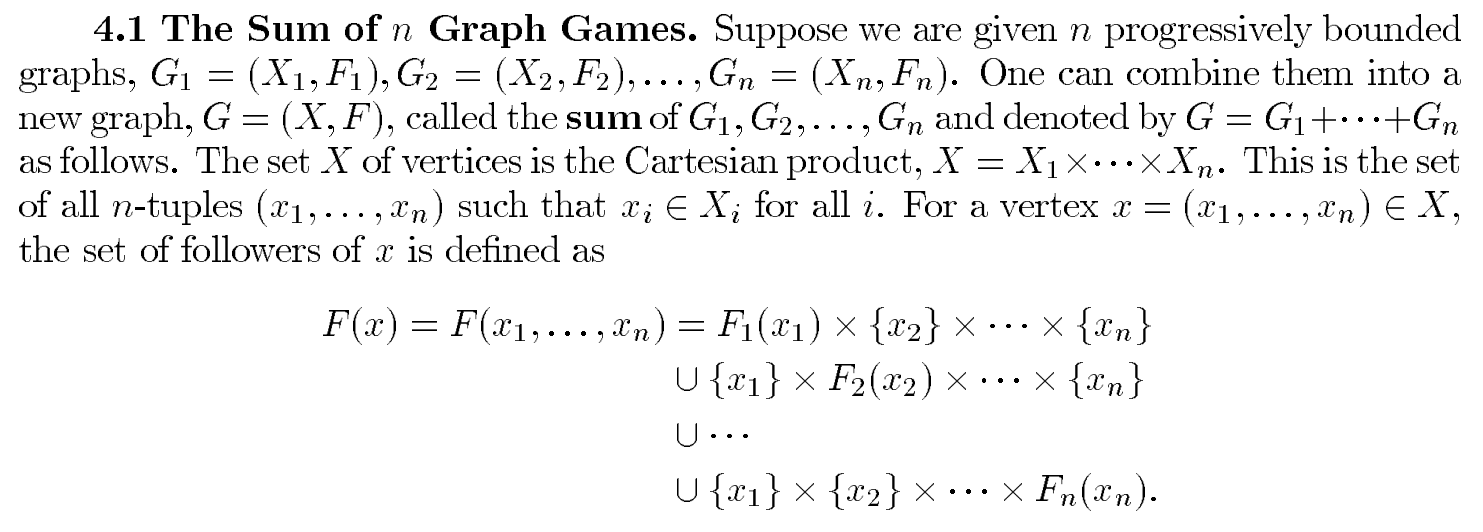
\includegraphics[width=0.5\textwidth,height=0.5\textheight,keepaspectratio]{sumgraph}
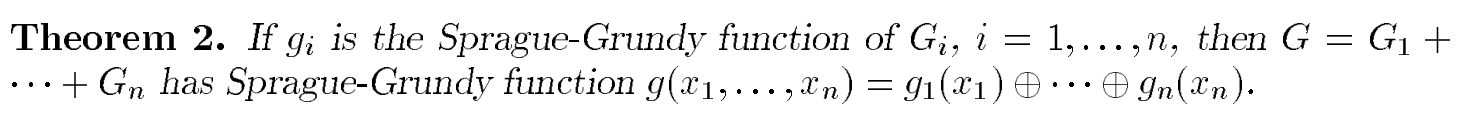
\includegraphics[width=0.5\textwidth,height=0.5\textheight,keepaspectratio]{sgth}
\textbf{Thus}, if a position is a \textbf{N} position, we can cleverly see which position should we go to (what move of a component game to take) such that we reach \textbf {P} position.
\subsection{Mobius}
Just read \href{https://github.com/sourabh2311/Competitive-Programming/blob/master/Reference%20Notes/Multiplicative.pdf}{this} and \href{https://www.quora.com/profile/Surya-Kiran/Posts/A-Dance-with-Mobius-Function}{this}.
\\\href{https://codeforces.com/contest/915/problem/G}{Prob}, \href{https://github.com/sourabh2311/Competitive-Programming/blob/master/CF/ER36/G.cpp}{Sol: }$\sum_{g = 1}^{i}h(g)*cnt[g]$ where $cnt[g] = $ no. of arrays with $gcd(a_1, a_2, a_3, ..., a_n) = g$ and where each $a_k \leq i$. Now $h(g) = $ Dirichlet identity function. Thus it is summation of mobius function. Ans thus we get $\sum_{d = 1}^{i}\mu(d)*f(d)$ where $f(d)$ is the number of arrays with elements in range $[1, i]$ such that $gcd(a_1, \dots, a_n)$ is divisible by $j$. Obviously $f(j) = (\lfloor i/j \rfloor)^n$.
\subsection{Bell, Burnside, etc}
Just read \href{https://github.com/sourabh2311/Competitive-Programming/blob/master/Reference%20Notes/cgt.pdf}{this}
\\Stirling no. of second kind obey the recurrence $$\stirling{n + 1}{k} = k * \stirling{n}{k} + \stirling{n}{k - 1} \forall n, k > 0$$ where $\stirling{0}{0} = 1$, $\stirling{n}{0} = \stirling{0}{n} = 0$
\\$\frac{1}{k!}\sum_{j=0}^{k}(-1)^{k-j}\binom{k}{j}j^n$
\subsubsection{Inclusion Exclusion Principle}
$$\left|\bigcup_{i=1}^n A_i \right| = \sum_{\emptyset \neq J\subseteq \{1,2,\ldots ,n\}} (-1)^{|J|-1}{\Biggl |}\bigcap_{j\in J}A_{j}{\Biggr |}$$
$$|\bigcap_{i = 1}^n A_{i}^c| = total - |\bigcap_{i = 1}^n A_i|$$
\subsection{Modulo}
$(a + b) mod m = (a mod m + b mod m) mod m$\\
$.........................-...............$\\
$.........................*...............$\\
\begin{minted}{cpp}
const int m1 = (int) 1e9 + 7;
template <typename T>
inline T add(T a, T b) {
    a += b;
    if (a >= m1) a -= m1;
    return a;
}
template <typename T>
inline T sub(T a, T b) {
    a -= b;
    if (a < 0) a += m1;
    return a;
}

template <typename T>
inline T mul(T a, T b) {
    return (T) (((long long) a * b) % m1);
}

template <typename T>
inline T power(T a, T b) {
    int res = 1;
    while (b > 0) {
        if (b & 1) {
            res = mul<T>(res, a);
        }
        a = mul<T>(a, a);
        b >>= 1;
    }
    return res;
}

template <typename T>
inline T inv(T a) {
    return power<T>(a, m1 - 2);
}
\end{minted}
\subsection{Prob and Comb}
\begin{itemize}
    \item $E[X] = \sum E(X|A_i)P(A_i)$
    \item \href {https://codeforces.com/contest/908/problem/D}{k, $p_a$, $p_b$ prob}, \href {https://github.com/sourabh2311/Competitive-Programming/blob/master/CF/Good%20Bye%202017/D.cpp}{Sol}, if $n + m \geq k \rightarrow p_b(i + j) + p_a*p_b*(i + j + 1) + p_a^2*p_b*(i + j + 2)\dots = (i + j) + \frac{p_a}{p_b}$ Also
    \begin{eqnarray}
    dp[0][0] & = & p_a * dp[1][0] + p_b * dp[0][0]\\
             & = & p_a * dp[1][0] / (1 - p_b)\\
             & = & dp[1][0]
    \end{eqnarray}
    \item \textbf{Dearrangement of n objects}
    \\ $n! * \sum_{k = 0}^n (-1)^k / {k!} =\text{ } !n$
    \\ $!n = (n - 1) * [!(n - 1) + !(n - 2)] \text{ for n }\geq 2$
    \item \textbf{Gambler ruin's problem: }Probability that first player (p for each step) wins. $(1 - (q/p)^{n_1})/(1 - (q/p)^{n_1 + n_2})$. $n_1 = \lceil ev_1/d \rceil$, $n_2 = \lceil ev_2/d \rceil$. In case $p = q = 1/2$, formula is $n_1/(n_1 + n_2)$.
    \item \href{}{UVA 10491}, $ans = (N_{cows} / (N_{cows} + N_{cars})) * (N_{cars} / (N_{cows} + N_{cars} - N_{shows} - 1)) + (N_{cars} / (N_{cows} + N_{cars})) * ((N_{cars} - 1) / (N_{cows} + N_{cars} - N_{shows} - 1))$
    \item $\binom{n}{r} = \binom{n - 1}{r - 1} + \binom{n - 1}{r}$
    \item $\binom{n}{r} = n / r * \binom{n - 1}{r - 1}$
    \item $\sum_{r = 0}^n \binom{n}{r} = 2^n$
    \item $\sum_{m = 0}^n \binom{m}{r} = \binom{n + 1}{r + 1}$
    \item $\sum_{k = 0}^m \binom{n + k}{k} = \binom{n + m - 1}{m}$
    \item $\sum_{i = 0}^n \binom{n}{i}^2 = \binom{2n}{n}$
\end{itemize}
\subsection{Placing Bishops on a Chessboard}

Find the number of ways to place $K$ bishops on an $N \times N$ chessboard so that no two bishops attack each other.
\subsubsection{Algorithm}

This problem can be solved using dynamic programming.

Let's enumerate the diagonals of the chessboard as follows: black diagonals have odd indices, white diagonals have even indices, and the diagonals are numbered in non-decreasing order of the number of squares in them. Here is an example for a $5 \times 5$ chessboard.

\[\begin{bmatrix} \bf{1} & 2 & \bf{5} & 6 & \bf{9} \\\
2 & \bf{5} & 6 & \bf{9} & 8 \\
\bf{5} & 6 & \bf{9} & 8 & \bf{7} \\
6 & \bf{9} & 8 & \bf{7} & 4 \\
\bf{9} & 8 & \bf{7} & 4 & \bf{3} \\
\end{bmatrix}\]

Let D[i][j] denote the number of ways to place j bishops on diagonals with indices up to i which have the same color as diagonal i. Then i = 1...2N-1 and j = 0...K.

We can calculate D[i][j] using only values of D[i-2] (we subtract 2 because we only consider diagonals of the same color as $i$). There are two ways to get D[i][j]. Either we place all j bishops on previous diagonals: then there are D[i-2][j] ways to achieve this. Or we place one bishop on diagonal i and j-1 bishops on previous diagonals. The number of ways to do this equals the number of squares in diagonal i minus j-1, because each of j-1 bishops placed on previous diagonals will block one square on the current diagonal. The number of squares in diagonal i can be calculated as follows:
\begin{minted}{cpp}
int squares (int i) {
    if (i & 1)
        return i / 4 * 2 + 1;
    else
        return (i - 1) / 4 * 2 + 2;
}
\end{minted}
The base case is simple: D[i][0] = 1, D[1][1] = 1.

Once we have calculated all values of D[i][j], the answer can be obtained as follows: consider all possible numbers of bishops placed on black diagonals i=0...K, with corresponding numbers of bishops on white diagonals K-i. The bishops placed on black and white diagonals never attack each other, so the placements can be done independently. The index of the last black diagonal is 2N-1, the last white one is 2N-2. For each i we add D[2N-1][i] * D[2N-2][K-i] to the answer.
\subsubsection{Implementation}
\begin{minted}{cpp}
int bishop_placements(int N, int K)
{
    if (K > 2 * N - 1)
        return 0;

    vector<vector<int>> D(N * 2, vector<int>(K + 1));
    for (int i = 0; i < N * 2; ++i)
        D[i][0] = 1;
    D[1][1] = 1;
    for (int i = 2; i < N * 2; ++i)
        for (int j = 1; j <= K; ++j)
            D[i][j] = D[i-2][j] + D[i-2][j-1] * (squares(i) - j + 1);

    int ans = 0;
    for (int i = 0; i <= K; ++i)
        ans += D[N*2-1][i] * D[N*2-2][K-i];
    return ans;
}
\end{minted}
\subsection{Euler's Totient Function}
Also known as phi-function $\phi (n)$, counts the number of integers between 1 and $n$ inclusive, which are coprime to $n$.
\\If $p$ is prime $\phi (p) = p - 1.$
\\If $p$ is a prime number and $k \ge 1$, then there are exactly $p^k / p$ numbers between $1$ and $p^k$ that are divisible by $p$. Which gives us:$\phi(p^k) = p^k - p^{k-1}.$
\\If $a$ and $b$ are relatively prime, then: $\phi(a b) = \phi(a) \cdot \phi(b).$ This relation is not trivial to see. It follows from the Chinese remainder theorem.
\\In general, for not coprime $a$ and $b$, the equation $$\phi(ab) = \phi(a) \cdot \phi(b) \cdot \dfrac{d}{\phi(d)}$$ with $d = \gcd(a, b)$ holds.\\
$ \phi (n) = \phi ({p_1}^{a_1}) \cdot \phi ({p_2}^{a_2}) \cdots \phi ({p_k}^{a_k})$\\
$ = \left({p_1}^{a_1} - {p_1}^{a_1 - 1}\right) \cdot \left({p_2}^{a_2} - {p_2}^{a_2 - 1}\right) \cdots \left({p_k}^{a_k} - {p_k}^{a_k - 1}\right)$\\
$ = p_1^{a_1} \cdot \left(1 - \frac{1}{p_1}\right) \cdot p_2^{a_2} \cdot \left(1 - \frac{1}{p_2}\right) \cdots p_k^{a_k} \cdot \left(1 - \frac{1}{p_k}\right)$ \\ 
$= n \cdot \left(1 - \frac{1}{p_1}\right) \cdot \left(1 - \frac{1}{p_2}\right) \cdots \left(1 - \frac{1}{p_k}\right) $\\
\textbf{Eulers Theorem: }\\
$$a^{\phi(m)} \equiv 1 \pmod m$$ if $a$ and $m$ are relatively prime.

In the particular case when $m$ is prime, Euler's theorem turns into Fermat's little theorem: $$a^{m - 1} \equiv 1 \pmod m$$
\\Converse of euler theorem is also true i.e. if $a^{\phi(m)} \equiv 1 (\mod n)$ then a and n must be coprime.
\subsection{Catalan}
$Cat(n) = \binom{2n}{n} / (n + 1)$
\\$Cat(m) = (2m*(2m - 1)/(m*(m + 1))) * Cat(m - 1)$
\\$Cat(n) = $\begin{enumerate}
    \item the number of ways a convex polygon with n+2 sides can be cut into n triangles
    \item the number of ways to use n rectangles to tile a stairstep shape (1, 2, ..., n−1, n).
    \item No. of expressions containing n pairs of parentheses which are correctly matched.
    \item the number of planar binary trees with n+1 leaves
    \item No. of distinct binary trees with n vertices
    \item No. of different ways in which n + 1 factors can be completely parenthesized. Like for \{a, b, c, d\}, one parenthing will be ((ab)c)d.
    \item the number of monotonic paths of length 2n through an n-by-n grid that do not rise above the main diagonal
    \item n pair of people on circle can do non cross hand shakes. i.e. no of ways to connect the 2n points on a circle to form n disjoint chords
    \item no. of permutations of length n that an be stack sorted
    \item no. of non crossing partitions of a set of n elements
\end{enumerate}
\textbf{Note: }Its better to use bigint for catalan computations. Also no. of binary trees with n labelled nodes $= cat[n] * fact[n]$
\subsection{Floyd Cycle Finding}
\begin{minted}{cpp}
// mu = start of the cycle
// lam = its length
// O (mu + lam) time complexity
// O (1) space complexity
ii floydCycleFinding(int x0) {
    // 1st part: finding k * lam
    int tortoise = f(x0), hare = f (f (x0));
    // hare moves at twice speed
    while (tortoise != hare) {
        tortoise = f (tortoise); hare = f(f(hare));
    }
    // thus tor = x_i; hare = x_2i
    // i.e. x_2i = x_{i + k * lam}
    // i.e. k * lam = i.
    // Now if hare is set to beginning
    // i.e. hare = x_0, tor = x_i
    // thus if both now move same no. of steps and in between they become equal, i.e.
    // x_l = x_{i + l}
    // i.e. x_l = x_{l + k * lam}
    // Thus l must be the minimum index and therefore l = mu
    int mu = 0;
    hare = x0;
    while (tortoise != hare) {
        tortoise = f (tortoise); hare = f(hare); mu++
    }
    // finding lam
    int lam = 1; hare = f (tortoise);
    while (tortoise != hare) {
        hare = f (hare); lambda++;
    }
    return ii (mu, lambda);
}
\end{minted}
\subsection{Base Conversion}
\begin{minted}{cpp}
// decimal no. to some base
stack<int> S;
while (q) {
    s.push (q % b);
    q /= b;
}
while (!s.empty ()) {
    cout << process (s.top ()) << " ";
    s.pop ();
}
// base to decimal no.
ll baseToDec () {
    ll ret = 0;
    for (auto &c : num) {
        ret = (ret * base + (c - 48)); // can take mod if final answer is required in mod
    }
    return ret;
}
\end{minted}
\subsection{Extended Euclid}
$ax + by = c$ this is called diophantine eqn and is solvable only when $d = gcd(a, b)$ divides c. so first solve $ax + by = d$ then multiply x, y with $c / d$. Also once we have found a particular soln to this eqn then their exist infinite solns of the form $(x0 + (b/d)*n, y0 - (a/d)*n)$ where n is any integer, note that these infinite solutions are as well the solution to original diophantine eqn. Assume we found the coefs (x1, y1) for (b, a mod b) $\rightarrow$ $b*x1 + (a\text{ mod }b)y1 = g\\ \rightarrow b*x1 + (a - \lfloor(a/b)\rfloor*b)*y1=g\\
\rightarrow a*y1 + b*(x1 - \lfloor (a/b)\rfloor * y1) = g\\
\rightarrow x = y1\text{ \& }y = x1 - \lfloor (a/b)\rfloor*y1$
\begin{minted}{cpp}
void extendedEuclid(int a, int b) {
   if (b == 0) { x = 1; y = 0; d = a; return; } // base case
   extendedEuclid(b, a % b); // similar as the original gcd
   int x1 = y;
   int y1 = x - (a / b) * y;
   x = x1;
   y = y1;
}
\end{minted}
\href{https://codeforces.com/problemsets/acmsguru/problem/99999/106}{SGU 106 Equation}, \href{https://github.com/sourabh2311/Competitive-Programming/blob/master/IMP%20QUES/Extended%20Euclid/106-The%20Equation.cpp}{Sol}
\\Prob: To find the soln with minimum value of $x + y$ and obviously there has to be range of x, y. Sol: Now $x + y = x_0 + y_0 + n * (b/d - a/d)$. If $a < b$, select smallest possible value of n. If $a > b$ select the largest. And if $a = b$, all solutions have same sum of $x + y$
\subsection{Linear Congruence Equation}
This equation is of the form:
$$a \cdot x = b \pmod n,$$

where $a$, $b$ and $n$ are given integers and $x$ is an unknown integer.

It is required to find the value $x$ from the interval $[0, n-1]$ (clearly, on the entire number line there can be infinitely many solutions that will differ from each other in $n \cdot k$ , where $k$ is any integer). If the solution is not unique, then we will consider how to get all the solutions.
\subsubsection{Solution by finding the inverse element}

Let us first consider a simpler case where $a$ and $n$ are coprime ($\gcd(a, n) = 1$). Then one can find the inverse of $a$, and multiplying both sides of the equation with the inverse, and we can get a unique solution.

$$x = b \cdot a ^ {- 1} \pmod n$$

Now consider the case where $a$ and $n$ are not coprime ($\gcd(a, n) \ne 1$). Then the solution will not always exist (for example $2 \cdot x = 1 \pmod 4$ has no solution).

Let $g = \gcd(a, n)$, i.e. the greatest common divisor of $a$ and $n$ (which in this case is greater than one).

Then, if $b$ is not divisible by $g$, there is no solution. In fact, for any $x$ the left side of the equation $a \cdot x \pmod n$ , is always divisible by $g$, while the right-hand side is not divisible by it, hence it follows that there are no solutions.

If $g$ divides $b$, then by dividing both sides of the equation by $g$ (i.e. dividing $a$, $b$ and $n$ by $g$), we receive a new equation:

$$a^\prime \cdot x = b^\prime \pmod{n^\prime}$$

in which $a^\prime$ and $n^\prime$ are already relatively prime, and we have already learned how to handle such an equation. We get $x^\prime$ as solution for $x$.

It is clear that this $x^\prime$ will also be a solution of the original equation. However it will not be the only solution. It can be shown that the original equation has exactly $g$ solutions, and they will look like this:

$$x_i = (x^\prime + i\cdot n^\prime) \pmod n \quad \text{for } i = 0 \ldots g-1$$

Summarizing, we can say that the number of solutions of the linear congruence equation is equal to either $g = \gcd(a, n)$ or to zero.
\subsubsection{Solution with the Advanced Euclidean Algorithm}

We can rewrite the linear congruence to the following Diophantine equation:

$$a \cdot x + n \cdot k = b,$$

where $x$ and $k$ are unknown integers.

The method of solving this equation is described in the corresponding article Linear Diophantine equations and it consists of applying the Extended Euclidean Algorithm.

It also describes the method of obtaining all solutions of this equation from one found solution, and incidentally this method, when carefully considered, is absolutely equivalent to the method described in the previous section.
\subsection{Sieve}
\begin{minted}{cpp}
    ll _sieve_size; // ll is defined as: typedef long long ll;
bitset<10000010> bs; // 10^7 should be enough for most cases
vi primes; // compact list of primes in form of vector<int>
void sieve(ll upperbound) { // create list of primes in [0..upperbound]
   _sieve_size = upperbound + 1; // add 1 to include upperbound
   bs.set(); // set all bits to 1
   bs[0] = bs[1] = 0; // except index 0 and 1
   for (ll i = 2; i <= _sieve_size; i++) if (bs[i]) {
// cross out multiples of i starting from i * i!
           for (ll j = i * i; j <= _sieve_size; j += i) bs[j] = 0;
           primes.push_back((int)i); // add this prime to the list of primes
       } } // call this method in main method
bool isPrime(ll N) { // a good enough deterministic prime tester
    // O(#primes < sqrt(N))
    // O(sqrt(N)/ln(sqrt(N)))
   if (N <= _sieve_size) return bs[N]; // O(1) for small primes
   for (int i = 0; i < (int)primes.size(); i++)
       if (N % primes[i] == 0) return false;
   return true; // it takes longer time if N is a large prime!
} // note: only work for N <= (last prime in vi "primes")^2

vi primeFactors(ll N) { // remember: vi is vector<int>, ll is long long
   vi factors;
   ll PF_idx = 0, PF = primes[PF_idx]; // primes has been populated by sieve
   while (PF * PF <= N) { // stop at sqrt(N); N can get smaller
       while (N % PF == 0) { N /= PF; factors.push_back(PF); } // remove PF
       PF = primes[++PF_idx]; // only consider primes!
   }
   if (N != 1) factors.push_back(N); // special case if N is a prime
   return factors; // if N does not fit in 32-bit integer and is a prime
} // then ‘factors’ will have to be changed to vector<ll>


memset(numDiffPF, 0, sizeof numDiffPF);
//Modified Sieve.
void pre() {
   for (int i = 2; i < MAX_N; i++)
       if (numDiffPF[i] == 0) // i is a prime number
           for (int j = i; j < MAX_N; j += i)
               numDiffPF[j]++; // increase the values of multiples of i
}
// Bottom up euler totient function
for (int i = 0; i <= limit; i++) eu[i] = i;
for (int i = 2; i <= limit; i++) {
    if (eu[i] == i) {
        for (int j = i; j <= limit; j += i) {
            eu[j] -= eu[j] / i;
        }
    }
}
\end{minted}
\subsection{Matrix}
Rank of a matrix is defined as 
\begin{itemize}
    \item Max. no. of linearly independent column vectors in the matrix or
    \item the max. no. of linearly independent row vectors in the matrix.
\end{itemize}
Both definitions are equivalent
\\For an r x c matrix
\begin{itemize}
    \item max rank = min (r, c)
    \item rank = no. of non zero rows of matrix in RREF.
\end{itemize}
To explain how gaussian elimination allows the computation of the determinant of a square matrix, we should know
\begin{itemize}
    \item Swapping two rows multiplies the determinant by -1
    \item Multiplying a row by a non zero scalar multiplies the determinant by same scalar
    \item Adding to one row a scalar multiple of another does not change the determinant
\end{itemize}
So if d is the product of scalar by which determinant has been multiplied having matrix in row echelon form, we have $det(A) = (\prod diag(B))/d$
\\To find inverse of the matrix augment it with identity matrix and get it RREF, if left block is identity matrix $\rightarrow$ right block is inverse. 
\subsection{Frac lib and Eqn solving}
\revised
\begin{minted}{cpp}
class Frac {
public:
   long long a, b;
   Frac() {
       a = 0, b = 1;
   }
   Frac(int x, int y) {
       a = x, b = y;
       reduce(); ///So we are always reducing out fractions...
   }
   Frac operator+(const Frac &y) {
       long long ta, tb;
       tb = this->b/gcd(this->b, y.b)*y.b;
       ta = this->a*(tb/this->b) + y.a*(tb/y.b);
       Frac z(ta, tb);
       return z;
   }
   Frac operator-(const Frac &y) {
       long long ta, tb;
       tb = this->b/gcd(this->b, y.b)*y.b;
       ta = this->a*(tb/this->b) - y.a*(tb/y.b);
       Frac z(ta, tb);
       return z;
   }
   Frac operator*(const Frac &y) {
       long long tx, ty, tz, tw, g;
       tx = this->a, ty = y.b;
       g = gcd(tx, ty), tx /= g, ty /= g;
       tz = this->b, tw = y.a;
       g = gcd(tz, tw), tz /= g, tw /= g;
       Frac z(tx*tw, ty*tz);
       return z;
   }
   Frac operator/(const Frac &y) {
       long long tx, ty, tz, tw, g;
       tx = this->a, ty = y.a;
       g = gcd(tx, ty), tx /= g, ty /= g;
       tz = this->b, tw = y.b;
       g = gcd(tz, tw), tz /= g, tw /= g;
       Frac z(tx*tw, ty*tz);
       return z;
   }
   bool operator == (const frac &other) const {
        return a == other.a and b == other.b;
    }
    bool operator < (const frac &other) const {
        if (a != other.a) return a < other.a;
        else return b > other.b;
    }
private:
   static long long gcd(long long x, long long y) {
       return b == 0 ? a : gcd (b, a % b);
   }
   void reduce() {
       if (a == 0) {  // to handle case when b == 0 (not required in this problem) a = inf (so as to have same ground)
           b = 1;
           return;
       } else {
            long long g = gcd(abs(a), abs(b));
            a /= g, b /= g;
            if(b < 0)   a *= -1, b *= -1;
       }
   }
    
};
ostream& operator<<(ostream& out, const Frac&x) {
   out << x.a;
   if(x.b != 1)
       out << '/' << x.b;
   return out;
}
int main() {//UVA 10109
   int n, m, i, j, k, N;
   char NUM[100], first = 0;
   long long X, Y;
   Frac matrix[100][100];
   while(scanf("%d", &N) == 1 && N) {
       scanf("%d %d", &n, &m);
       for(i = 0; i < m; i++) {
           for(j = 0; j <= n; j++) {
               scanf("%s", NUM);
               if(sscanf(NUM, "%lld/%lld", &X, &Y) == 2) {
                   matrix[i][j].a = X;
                   matrix[i][j].b = Y;
               } else
                   sscanf(NUM, "%lld", &matrix[i][j].a), matrix[i][j].b = 1;
           }
       }
       Frac tmp, one(1,1);
       int idx = 0, rank = 0;
       for(i = 0; i < m; i++) {
           while(idx < n) {
               int ch = -1;
               for(j = i; j < m; j++)
                   if(matrix[j][idx].a) {///This means that idx must be incremented to check
                       ///the pivot at correct row...
                       ch = j;
                       break;
                   }
               if(ch == -1) {
                   idx++;
                   continue;
               }///this if condition executes if all the elements in desired column
               ///and below the i-1 th row are zero so we need to go to the next column...
               if(i != ch)///So if the desired pivot element is zero we swap that row with
                   ///the closest row that has non zero pivot...
                   for(j = idx; j <= n; j++)
                       swap(matrix[ch][j], matrix[i][j]);
               break;
           }
           if(idx >= n) break;
           tmp = one/matrix[i][idx];
           rank++;
           for(j = idx; j <= n; j++)
               matrix[i][j] = matrix[i][j]*tmp;///So here we are making pivot element 1.
           for(j = 0; j < m; j++) {
               if(i == j)  continue;///This condition executes means that we are ignoring the
               ///pivot row...
               tmp = matrix[j][i]/matrix[i][idx];
               for(k = idx; k <= n; k++) {
                   matrix[j][k] = matrix[j][k] - tmp*matrix[i][k];///Thus now we are making
                   ///all the elements below pivot as zero..
               }
           }
           idx++;
       }
       if(first)   puts("");
       first = 1;
       printf("Solution for Matrix System # %d\n", N);
       int sol = 0;
       for(i = 0; i < m; i++) {
           for(j = 0; j < n; j++) {
               if(matrix[i][j].a)
                   break;
           }
           if(j == n) {
               if(matrix[i][n].a == 0 && sol != 1)
                   sol = 0; // INFINITELY
               else
                   sol = 1; // No Solution.
           }
       }
       if(rank == n && sol == 0) {
           for(i = 0; i < n; i++) {
               printf("x[%d] = ", i+1);
               cout << matrix[i][n] << endl;
           }
           continue;
       }
       if(sol == 1)
           puts("No Solution.");
       else
           printf("Infinitely many solutions containing %d arbitrary constants.\n", n-rank);
   }
   return 0;
}
\end{minted}
\subsection{Balanced Ternary}
It is a ternary (base 3) no. system in which digits have values $-1, 0, 1$. Balanced ternary can represent all integers without using a seperate minus sign. To convert unbalanced ternary (0, 1, 2) to balanced ternary (which may have digits after a radix point) start from the right most digit and proceed towards left, if the digit is 0, 1, then ignore, but if it is 2, replace it with z and add 1 to the digit towards left.
\\Ex: $200120_{unbal} = 2002z0 = 201zz0 = 1z01zz0_{bal}$
\\Ex: $022_{unbal} = 0003z = 0010z_{bal}$
\\\href{https://apps.topcoder.com/wiki/display/tc/SRM+604}{Just see both the power of 3 problems}
\subsection{15 Puzzle Game: Existence Of The Solution}

This game is played on a $4 \times 4$ board. On this board there are 15 playing tiles numbered from 1 to 15. One cell is left empty (denoted by 0). You need to get the board to the position presented below by repeatedly moving one of the tiles to the free space:

$$\begin{matrix} 1 & 2 & 3 & 4 \\ 5 & 6 & 7 & 8 \\ 9 & 10 & 11 & 12 \\ 13 & 14 & 15 & 0 \end{matrix}$$

\subsubsection{Existence Of The Solution}j

Let's consider this problem: given position on the board, determine whether a sequence of moves which leads to a solution exists.

Suppose we have some position on the board:

$$\begin{matrix} a_1 & a_2 & a_3 & a_4 \\ a_5 & a_6 & a_7 & a_8 \\ a_9 & a_{10} & a_{11} & a_{12} \\ a_{13} & a_{14} & a_{15} & a_{16} \end{matrix}$$

where one of the elements equals zero and indicates an empty cell $a_z = 0$

Let’s consider the permutation:

$$a_1 a_2 ... a_{z-1} a_{z+1} ... a_{15} a_{16}$$

(i.e. the permutation of numbers corresponding to the position on the board without a zero element)

Let $N$ be the number of inversions in this permutation (i.e. the number of such elements $a_i$ and $a_j$ that $i > j$, but $a_i < a_j$).

Suppose $K$ is an index of a row where the empty element is located (i.e. in our indications $K = (z - 1) \ div \ 4 + 1$).

Then, the solution exists iff $N + K$ is even.
\subsection{Stern Broco Tree}
At zero iteration, we have 2 fractions (0/1 and 1/0) further at each subsequent iteration, this list of fractions is taken and between each 2 adjacent fractions a/b and c/d their median is inserted ($(a+c)/(b+d)$). It is stated that it is possible to obtain the set of all non negative fractions. Moreover all recieved fractions will be different and irreducible. Any tow adjacent fractions a/b, c/d with ($a/b < c/d$) satisfies $bc - ad = 1$, this statement aswell holds for farey sequence of any order. Converse is aswell true, so if a/b and c/d are first two terms and next term is p/q then $c/d = (p + a)/(b + q)$ Note that we cannot say $c = p + a, d = b + q$. So, $kc = a + p, kd = b + q$ i.e. $p(k) = kc - a, q(k) = kd - b$, and k happens to be $\lfloor(n + b)/d\rfloor$. Thus for constructing farey sequence of order n, we can start with a/b = 0/1 and c/d = 1/n.
\\Algo for constructing this tree:
\begin{minted}{cpp}
void build (int a = 0, int b = 1, int c = 1, int d = 0, int level = 1) {
    int x = a + c, y = b + d;
    build (a, b, x, y, level + 1);
    build (x, y, c, d, level + 1);
}
// Search algo for fractions, algo will not terminate irrational nos
string find (int x, int y, int a = 0, int b = 1, int c = 1, int d = 0) {
    int m = a + c, n = b + d;
    if (x == m and y == n) return "";
    if (x * n < y * m) return "L" + find (x, y, a, b, m, n);
    else return "R" + find (x, y, m, n, c, d);
}
\end{minted} 
\textbf{Farey sequence} of order n is the sequence of completely reduced fractions between 0 and 1 which when in irreducible form have denominators less than or equal to n, arranged in order of increasing size. $F_5 = \{0/1, 1/5, 1/4, 1/3, 2/5, 1/2, 3/5, 2/3, 3/4, 4/5, 1/1\}$
\\The order (n) farey sequence contains all the elements of farey sequence with order $n - 1$ and also all irreducible fractions with denominators equal to n but this no. is $\phi(n)$. Thus $L_n = L_{n - 1} + \phi(n) = 1 + \sum_{k = 1}^n \phi(k)$

\subsection{Finding Power Of Factorial Divisor}
You are given two numbers $n$ and $k$. Find the largest power of $k$ (say $x$) such that $n!$ is divisible by $k^x$.
\subsubsection{Prime $k$}

Let's first consider the case of prime $k$. The explicit expression for factorial

$$n! = 1 \cdot 2 \cdot 3 \ldots (n-1) \cdot n$$

Note that every $k$-th element of the product is divisible by $k$, i.e. adds $+1$ to the answer; the number of such elements is $\Bigl\lfloor\dfrac{n}{k}\Bigr\rfloor$.

Next, every $k^2$-th element is divisible by $k^2$, i.e. adds another $+1$ to the answer (the first power of $k$ has already been counted in the previous paragraph). The number of such elements is $\Bigl\lfloor\dfrac{n}{k^2}\Bigr\rfloor$.

And so on, for every $i$ each $k^i$-th element adds another $+1$ to the answer, and there are $\Bigl\lfloor\dfrac{n}{k^i}\Bigr\rfloor$ such elements.

The final answer is

$$\Bigl\lfloor\dfrac{n}{k}\Bigr\rfloor + \Bigl\lfloor\dfrac{n}{k^2}\Bigr\rfloor + \ldots + \Bigl\lfloor\dfrac{n}{k^i}\Bigr\rfloor + \ldots$$

The sum is of course finite, since only approximately the first $\log_k n$ elements are not zeros. Thus, the runtime of this algorithm is $O(\log_k n)$.
Implementation:
\begin{minted}{cpp}
int fact_pow (int n, int k) {
	int res = 0;
	while (n) {
		n /= k;
		res += n;
	}
	return res;
}
\end{minted}
\subsubsection{Composite $k$}

The same idea can't be applied directly. Instead we can factor $k$, representing it as $k = k_1^{p_1} \cdot \ldots \cdot k_m^{p_m}$. For each $k_i$, we find the number of times it is present in $n!$ using the algorithm described above - let's call this value $a_i$. The answer for composite $k$ will be

$$\min_ {i=1 \ldots m} \dfrac{a_i}{p_i}$$
\subsection{GCD, LCM}
\begin{minted}{cpp}
    // time complexity O(log(min(a, b) / gcd(a, b)))
    int gcd (int a, int b) { return b == 0 ? a : gcd (b, a % b); }
    int lcm (int a, int b) { return a * (b / gcd (a, b)); }
\end{minted}
\begin{itemize}
    \item For a series of numbers if you want next no. to have gcd 1 with all previous no. then $GCD(a_j, LCM(a_1, a_2, \dots, a_{j - 1})) = 1$.
    \item if $p|N \& p|M$ then $p|gcd(N, M)$ as $N = pk, M = pl \rightarrow$ N, M have p common so gcd will also have p.
    \item $N|P \& M|P \rightarrow lcm(N, M)|P$.
    \item $N = gcd(N, m) \Leftrightarrow N|M$
    \item $M = lcdm(N, M) \Leftrightarrow N|M$
    \item $gcd(P*N, P*M) = P*gcd(N, M)$
    \item $lcm(P*N, P*M) = P*lcm(N, M)$
    \item If $gcd(N_1, N_2) = 1$ then $gcd(N_1 * N_2, M) = gcd(N_1, M) * gcd(N_2, M)$ and $lcm(N_1*N_2, M) = lcm(N_1, M)*lcm(N_2, M)/M$
    \item gcd(gcd(N, M), P) = gcd(N, gcd(M, P))
    \item lcm(lcm(N, M), P) = lcm(N, lcm(M, P))
    \item gcd(M, N, P) = gcd(gcd(M, N), P) = gcd(M, gcd(N, P))
    \item lcm(M, N, P) = lcm(lcm(M, N), P) = lcm(M, lcm(N, P))
    \item for integers $N_1, \dots, N_k$ and $k \geq 2$, 
    $$lcm(gcd(N_1, M), gcd(N_2, M), \dots, gcd(N_k, M)) = gcd(lcm(N_1, \dots, N_k), M)$$
    $$gcd(lcm(N_1, M), lcm(N_2, M), \dots, lcm(N_k, M)) = lcm(gcd(N_1, \dots, N_k), M)$$
\end{itemize}
\subsection{Some properties of Fibonacci numbers}
\begin{itemize}
    \item $F_0 = 0, F_1 = 1, F_n = F_{n-1} + F_{n-2}$
    \item Cassini's identity: $F_{n-1} F_{n+1} - F_n^2 = (-1)^n$
    \item The "addition" rule: $F_{n+k} = F_k F_{n+1} + F_{k-1} F_n$
    \item Applying the previous identity to the case $k = n$, we get: $F_{2n} = F_n (F_{n+1} + F_{n-1})$
    \item From this we can prove by induction that for any positive integer $k$, $F_{nk}$ is multiple of $F_n$.
    The inverse is also true: if $F_m$ is multiple of $F_n$, then $m$ is multiple of $n$.
    \item GCD identity: $GCD(F_m, F_n) = F_{GCD(m, n)}$
    \item Every positive integer can be expressed uniquely as a sum of fibonacci numbers such that no two numbers are equal or consecutive fibonacci numbers. This can be done greedily by taking the highest fibonacci no. at each point.
    \item Fibonacci nos are periodic under modulo. The period of the fibonacci sequence modula a positive integer j is the smallest positive integer m such that such that $F_m \equiv 0 (mod j) \& F_{m + 1} \equiv 1 (mod j)$
    \item \[\begin{bmatrix}
    1 & 1\\
    1 & 0
    \end{bmatrix}^{\!p}
=
\begin{bmatrix}
    fib(p + 1) & fib (p)\\
    fib (p) & fib (p - 1)
    \end{bmatrix}
    \]
    \textit{Thus higher fibs can be computed in $O(\log{p})$}
    \item $$F_n = \frac{\left(\frac{1 + \sqrt{5}}{2}\right)^n - \left(\frac{1 - \sqrt{5}}{2}\right)^n}{\sqrt{5}}$$
    \item You can immediately notice that the second term's absolute value is always less than $1$, and it also decreases very rapidly (exponentially). Hence the value of the first term alone is "almost" $F_n$. This can be written strictly as:
    $$F_n = \left[\frac{\left(\frac{1 + \sqrt{5}}{2}\right)^n}{\sqrt{5}}\right]$$
\end{itemize}
\subsection{Wilson Theorem}
States that for a prime no. p, $(p - 1)! \mod p = p - 1$.
\\Note that $n! \mod p$ is 0 if $n \geq p$. Suppose p is prime and is close to input number n. For example $25! \mod 29$. From wilson theorem, we know that $28! \mod 29 = -1 \equiv 28$, so we basically need to find $(28 * inverse(28, 29) * inverse (27, 29) * inverse (26, 29)) \mod 29$
\\Time complexity $O((p - n) * \log n)$
\subsection{Factorial modulo $p$ in $O(p \log n)$}
In some cases it is necessary to consider complex formulas modulo $p$, containing factorials in both numerator and denominator. We consider the case when $p$ is relatively small. This problem makes sense only when factorials are included in both numerator and denominator of fractions. Otherwise $p!$ and subsequent terms will reduce to zero, but in fractions all multipliers containing $p$ can be reduced, and the resulting expression will be non-zero modulo $p$.

Thus, formally the task is: You want to calculate $n! \bmod p$, without taking all the multiple factors of $p$ into account that appear in the factorial. Imaging you write down the prime factorization of $n!$, remove all factors $p$, and compute the product modulo $p$. We will denote this modified factorial with $n!_{\mod p}$.

Learning how to effectively calculate this modified factorial allows us to quickly calculate the value of the various combinatorial formulae (for example, Binomial coefficients).

\subsubsection{Algorithm}
Let's write this modified factorial explicitly.

\begin{eqnarray} n!_{\mod p} &=& 1 \cdot 2 \cdot 3 \cdot \ldots \cdot (p-2) \cdot (p-1) \cdot \underbrace{1}_{p} \cdot (p+1) \cdot (p+2) \cdot \ldots \cdot (2p-1) \cdot \underbrace{2}_{2p} \\
& &\quad \cdot (2p+1) \cdot \ldots \cdot (p^2-1) \cdot \underbrace{1}_{p^2} \cdot (p^2 +1) \cdot \ldots \cdot n \pmod{p} \\ &=& 1 \cdot 2 \cdot 3 \cdot \ldots \cdot (p-2) \cdot (p-1) \cdot \underbrace{1}_{p} \cdot 2 \cdot \ldots \cdot (p-1) \cdot \underbrace{2}_{2p} \cdot 1 \cdot 2 \\
& &\quad \cdot \ldots \cdot (p-1) \cdot \underbrace{1}_{p^2} \cdot 1 \cdot 2 \cdot \ldots \cdot (n \bmod p) \pmod{p} \end{eqnarray}

It can be clearly seen that factorial is divided into several blocks of same length expect for the last one.

\noindent\begin{eqnarray} n!_{\mod p}&=& \underbrace{1 \cdot 2 \cdot 3 \cdot \ldots \cdot (p-2) \cdot (p-1) \cdot 1}_{1\text{st}} \cdot \underbrace{1 \cdot 2 \cdot 3 \cdot \ldots \cdot (p-2) \cdot (p-1) \cdot 2}_{2\text{nd}} \cdot \ldots \\ & & \cdot \underbrace{1 \cdot 2 \cdot 3 \cdot \ldots \cdot (p-2) \cdot (p-1) \cdot 1}_{p\text{th}} \cdot \ldots \cdot \quad \underbrace{1 \cdot 2 \cdot \cdot \ldots \cdot (n \bmod p)}_{\text{tail}} \pmod{p}. \end{eqnarray}

The general part of the blocks it is easy to count — it's just $(p-1)!\ \mathrm{mod}\ p$ that you can calculate programmatically or via Wilson theorem, according to which $(p-1)! \bmod p = p-1$. To multiply these common parts of all blocks, we can raise the value to the higher power modulo $p$, which can be done in $O(\log n)$ operations using Binary Exponentiation; however, you may notice that the result will always be either $1$ or $p-1$, depending on the parity of the index. The value of the last partial block can be calculated separately in $O(p)$. Leaving only the last elements of the blocks, we can examine that:

\noindent$$n!_{\mod p} = \underbrace{ \ldots \cdot 1 } \cdot \underbrace{ \ldots \cdot 2} \cdot \ldots \cdot \underbrace{ \ldots \cdot (p-1)} \cdot \underbrace{ \ldots \cdot 1 } \cdot \underbrace{ \ldots \cdot 1} \cdot \underbrace{ \ldots \cdot 2} \cdots$$

And again, by removing the blocks that we already computed, we receive a "modified" factorial but with smaller dimension ($\lfloor n / p \rfloor$ blocks remain). Thus, in the calculation of "modified" the factorial $n!{\mod p}$ we did $O(p)$ operations and are left with the calculation of $(n/p)!{\mod p}$. Revealing this recursive dependence, we obtain that the recursion depth is $O(\log_p n)$, the total asymptotic behavior of the algorithm is thus $O(p \log_p n)$.
\subsubsection{Implementation}
We don't need recursion because this is a case of tail recursion and thus can be easily implemented using iteration.
\begin{minted}{cpp}
int factmod(int n, int p) {
	int res = 1;
	while (n > 1) {
		res = (res * ((n/p) % 2 ?  p-1 : 1)) % p;
		for (int i = 2; i <= n%p; ++i)
			res = (res * i) % p;
		n /= p;
	}
	return res % p;
}
\end{minted}
This implementation works in $O(p \log_p n)$.
\subsection{Modular Inverse}
A modular multiplicative inverse of an integer $a$ is an integer $x$ such that $a \cdot x$ is congruent to $1$ modular some modulus $m$. $a \cdot x \equiv 1 \mod m.$ We will also denote $x$ with $a^{-1}$.

It can be proven that the modular inverse exists if and only if $a$ and $m$ are relatively prime (i.e. $\gcd(a, m) = 1$).

For an arbitrary (but coprime) modulus $m$: $a ^ {\phi (m) - 1} \equiv a ^{-1} \mod m$\\
For a prime modulus $m$: $a ^ {m - 2} \equiv a ^ {-1} \mod m$
From these results, we can easily find the modular inverse using the binary exponentiation algorithm, which works in O(logm) time.
\\Or
Consider the following equation (with unknown $x$ and $y$):

$$a \cdot x + m \cdot y = 1$$

This is a Linear Diophantine equation in two variables. As shown in the linked article, when $\gcd(a, m) = 1$, the equation has a solution which can be found using the extended Euclidean algorithm. Note that $\gcd(a, m) = 1$ is also the condition for the modular inverse to exist.

Now, if we take modulo $m$ of both sides, we can get rid of $m \cdot y$, and the equation becomes:

$$a \cdot x \equiv 1 \mod m$$

Thus, the modular inverse of $a$ is $x$.

The implementation is as follows:
\begin{minted}{cpp}
int x, y;
int g = extended_euclidean(a, m, x, y);
if (g != 1) {
    cout << "No solution!";
}
else {
    x = (x % m + m) % m;
    cout << x << endl;
}
\end{minted}
Notice that we way we modify x. The resulting x from the extended Euclidean algorithm may be negative, so x % m might also be negative, and we first have to add m to make it positive.

The problem is the following: we want to compute the modular inverse for every number in the range $[1, m-1]$.

Applying the algorithms described in the previous sections, we can obtain a solution with complexity $O(m \log m)$.

Here we present a better algorithm with complexity $O(m)$. However for this specific algorithm we require that the modulus $m$ is prime.

We denote by $\text{inv}[i]$ the modular inverse of $i$. Then for $i > 1$ the following equation is valid:

$$\text{inv}[i] = - \left\lfloor \frac{m}{i} \right\rfloor \cdot \text{inv}[m \bmod i] \bmod m$$

Thus the implementation is very simple:
\begin{minted}{cpp}
inv[1] = 1;
for(int i = 2; i < m; ++i)
    inv[i] = (m - (m/i) * inv[m%i] % m) % m;
\end{minted}
\textbf{Proof}

We have: $$m \bmod i = m - \left\lfloor \frac{m}{i} \right\rfloor \cdot i$$ Taking both sides modulo $m$ yields: $$m \bmod i \equiv - \left\lfloor \frac{m}{i} \right\rfloor \cdot i \mod m$$ Multiply both sides by $i^{-1} \cdot (m \bmod i)^{-1}$ yields $$(m \bmod i) \cdot i^{-1} \cdot (m \bmod i)^{-1} \equiv -\left\lfloor \frac{m}{i} \right\rfloor \cdot i \cdot i^{-1} \cdot (m \bmod i)^{-1} \mod m,$$ which simplifies to: $$i^{-1} \equiv -\left\lfloor \frac{m}{i} \right\rfloor \cdot (m \bmod i)^{-1} \mod m,$$
\\
\textbf{Binomial coeff modulo large prime no}
\begin{minted}{cpp}
fact[0] = 1;
for (int i = 1; i <= maxn; i++) {
    fact[i] = (fact[i - 1] * (i % m)) % m;
}
// afterwards we can compute binomial coeff in O(log m)
ll getC(int n, int k) {
    ll res = fact[n];
    ll div = fact[k] * fact[n - k] % m;
    div = pow (div, m - 2, m);
    return (res * div) % m;
}
\end{minted}
\textbf{Binomial Coeff modulo prime power}
Here we want to compute the binomial coefficient modulo some prime power, i.e. $m = p^b$ for some prime $p$. If $p > \max(k, n-k)$, then we can use the same method as described in the previous section. But if $p \le \max(k, n-k)$, then at least one of $k!$ and $(n-k)!$ are not coprime with $m$, and therefore we cannot compute the inverses - they don't exist. Nevertheless we can compute the binomial coefficient.

The idea is the following: We compute for each $x!$ the biggest exponent $c$ such that $p^c$ divides $x!$, i.e. $p^c | x!$. Let $c(x)$ be that number. And let $g(x) := \frac{x!}{p^{c(x)}}$. Then we can write the binomial coefficient as: $$\binom n k = \frac {g(n) p^{c(n)}} {g(k) p^{c(k)} g(n-k) p^{c(n-k)}} = \frac {g(n)} {g(k) g(n-k)}p^{c(n) - c(k) - c(n-k)}$$

The interesting thing is, that $g(x)$ is now free from the prime divisor $p$. Therefore $g(x)$ is coprime to m, and we can compute the modular inverses of $g(k)$ and $g(n-k)$.

After precomputing all values for $g$ and $c$, which can be done efficiently using dynamic programming in $\mathcal{O}(n)$, we can compute the binomial coefficient in $O(\log m)$ time. Or precompute all inverses and all powers of $p$, and then compute the binomial coefficient in $O(1)$.

Notice, if $c(n) - c(k) - c(n-k) \ge b$, than $p^b | p^{c(n) - c(k) - c(n-k)}$, and the binomial coefficient is $0$.
\\\textbf{Binomial coefficient modulo an arbitrary number}
Now we compute the binomial coefficient modulo some arbitrary modulus $m$.

Let the prime factorization of $m$ be $m = p_1^{e_1} p_2^{e_2} \cdots p_h^{e_h}$. We can compute the binomial coefficient modulo $p_i^{e_i}$ for every $i$. This gives us $h$ different congruences. Since all moduli $p_i^{e_i}$ are coprime, we can apply the Chinese Remainder Theorem to compute the binomial coefficient modulo the product of the moduli, which is the desired binomial coefficient modulo $m$.
\\%------------------------------------
\textbf{Lucas's theorem}
For non-negative integers m and n and a prime p, the following congruence relation holds:

    ${\binom {m}{n}}\equiv \prod _{i=0}^{k}{\binom {m_{i}}{n_{i}}}{\pmod {p}}$

where

    $m=m_{k}p^{k}+m_{k-1}p^{k-1}+\cdots +m_{1}p+m_{0}$

and

    $n=n_{k}p^{k}+n_{k-1}p^{k-1}+\cdots +n_{1}p+n_{0}$ 

are the base p expansions of m and n respectively. This uses the convention that  ${\tbinom {m}{n}}=0$ if m < n. 
\\\textbf{Binomial coefficient for large $n$ and small modulo}
When $n$ is too large, the $\mathcal{O}(n)$ algorithms discussed above become impractical. However, if the modulo $m$ is small there are still ways to calculate $\binom{n}{k} \bmod m$.

When the modulo $m$ is prime, there are 2 options:

    Lucas's theorem can be applied which breaks the problem of computing $\binom{n}{k} \bmod m$ into $\log_m n$ problems of the form $\binom{x_i}{y_i} \bmod m$ where $x_i, y_i < m$. If each reduced coefficient is calculated using precomputed factorials and inverse factorials, the complexity is $\mathcal{O}(m + \log_m n)$.
    \\The method of computing factorial modulo P can be used to get the required $g$ and $c$ values and use them as described in the section of modulo prime power. This takes $\mathcal{O}(m \log_m n)$.

When $m$ is not prime but square-free, the prime factors of $m$ can be obtained and the coefficient modulo each prime factor can be calculated using either of the above methods, and the overall answer can be obtained by the Chinese Remainder Theorem.

When $m$ is not square-free, a generalization of Lucas's theorem for prime powers can be applied instead of Lucas's theorem. I don't think that I need to consider that.
\subsection{Gray Code}
Gray code is a binary numeral system where two successive values differ in only one bit.

For example, the sequence of Gray codes for 3-bit numbers is: 000, 001, 011, 010, 110, 111, 101, 100, so $G(4) = 6$.
\subsubsection{Finding Gray Code}
Let's look at the bits of number $n$ and the bits of number $G(n)$. Notice that $i$-th bit of $G(n)$ equals 1 only when $i$-th bit of $n$ equals 1 and $i + 1$-th bit equals 0 or the other way around ($i$-th bit equals 0 and $i + 1$-th bit equals 1). Thus, $G(n) = n \oplus (n >> 1)$:
\begin{minted}{cpp}
int g (int n) {
    return n ^ (n >> 1);
}
\end{minted}
\subsubsection{Finding inverse gray code}
Given Gray code $g$, restore the original number $n$.

We will move from the most significant bits to the least significant ones (the least significant bit has index 1 and the most significant bit has index $k$). The relation between the bits $n_i$ of number $n$ and the bits $g_i$ of number $g$:

 \begin{eqnarray}n_k &= g_k, \\ n_{k-1} &= g_{k-1} \oplus n_k = g_k \oplus g_{k-1}, \\ n_{k-2} &= g_{k-2} \oplus n_{k-1} = g_k \oplus g_{k-1} \oplus g_{k-2}, \\ n_{k-3} &= g_{k-3} \oplus n_{k-2} = g_k \oplus g_{k-1} \oplus g_{k-2} \oplus g_{k-3}, \\ \vdots \end{eqnarray}

The easiest way to write it in code is:
\begin{minted}{cpp}
    int rev_g (int g) {
  int n = 0;
  for (; g; g >>= 1)
    n ^= g;
  return n;
}
\end{minted}

\href{https://codeforces.com/problemsets/acmsguru/problem/99999/249}{SGU 249 Matrix}, \href{https://github.com/sourabh2311/Competitive-Programming/blob/master/IMP%20QUES/Gray%20Code/SGU249-Matrix.cpp}{Sol}
\subsection{Discrete Logarithm}

The discrete logarithm is an integer $x$ solving the equation

$a^x \equiv b \pmod m$

where $a$ and $m$ are relatively prime. (Note: if they are not relatively prime, then the algorithm described below is incorrect, though it can be modified so that it can work).

In this article, we describe the Baby step - giant step algorithm, proposed by Shanks in 1971, which has complexity $O(\sqrt{m} \log m)$. This algorithm is also known as meet-in-the-middle, because of it uses technique separation of tasks in half.
\subsubsection{Algorithm}

Consider the equation:

$a^x \equiv b \pmod m$

where $a$ and $m$ are relatively prime.

Let $x = np - q$, where $n$ is some pre-selected constant (we will describe how to select $n$ later). $p$ is known as giant step, since increasing it by one increases $x$ by $n$. Similarly, $q$ is known as baby step.

Obviously, any value of $x$ in the interval $[0; m)$ can be represented in this form, where $p \in [1; \lceil \frac{m}{n} \rceil ]$ and $q \in [0; n]$.

Then, the equation becomes:

$a^{np - q} \equiv b \pmod m$.

Using the fact that $a$ and $m$ are relatively prime, we obtain:

$a^{np} \equiv ba^q \pmod m$

This new equation can be rewritten in a simplified form:

$f_1(p) = f_2(q)$.

This problem can be solved using the method meet-in-the-middle as follows:

    We calculate $f_1$ for all possible values of $p$. Sort these values.
    For each value of $q$, calculate $f_2$, and look for the corresponding value of $p$ using the sorted array of $f_1$ using binary search.

\subsubsection{Complexity}

For each value of $p$, we can calculate $f_1(p)$ in $O(\log m)$ using binary exponentation algorithm. Similar for $f_2(q)$.

In the first step of the algorithm, we need to calculate $f_1$ for every possible values of $p$, and then sort them. Thus, this step has complexity:

$O(\lceil \frac{m}{n} \rceil (\log m + \log \lceil \frac{m}{n} \rceil )) = O( \lceil \frac {m}{n} \rceil \log m)$

In the second step of the algorithm, we need to calculate $f_2(q)$ for each possible value of $q$, and then do a binary search on the array of values of $f_1$, thus this step has complexity:

$O(n (\log m + \log \frac{m}{n} ) ) = O(n \log m)$.

Now, when we add these two complexity, we would get $\log m$ multiplied by $n$ and $m/n$, which has minimum value when $n = m/n$, which means, to achieve optimal performance, $n$ should be chosen such that:

$n = \sqrt{m}$.

Then, the complexity of the algorithm becomes:

$O(\sqrt {m} \log m)$.
\subsubsection{Implementation}
The simplest implementation

In the following code, function powmod performs binary exponential $a^b \pmod m$, and function solve produces a proper solution to the problem. It will returns $-1$ if there is no solution, and returns one possible solution in case a solution exists.
\begin{minted}{cpp}
int powmod (int a, int b, int m) {
	int res = 1;
	while (b > 0)
		if (b & 1) {
			res = (res * a) % m;
			--b;
		}
		else {
			a = (a * a) % m;
			b >>= 1;
		}
	return res % m;
}
 
int solve (int a, int b, int m) {
	int n = (int) sqrt (m + .0) + 1;
	map<int,int> vals;
	for (int i=n; i>=1; --i)
		vals[ powmod (a, i * n, m) ] = i;
	for (int i=0; i<=n; ++i) {
		int cur = (powmod (a, i, m) * b) % m;
		if (vals.count(cur)) {
			int ans = vals[cur] * n - i;
			if (ans < m)
				return ans;
		}
	}
	return -1;
}
\end{minted}
In this code, we used map from C++ STL to store the values of $f_1 (i)$. Internally, map uses red-black-tree to store values. This code is a little bit slower than if we uses array and binary search for $f1$, but is much easier to write.

Another thing to note is that, if there are multiple values of $p$ that has same value of $f_1$, we only store one such value. This works in this case because we only want to return one possible solution. If we need to return all possible solutions, we need to change map<int,int> to, say, map<int, vector<int> >. And we also need to change the second step accordingly.
\subsubsection{Improved implementation}j

A possible improvement is to get rid of binary exponentiation in the second phase of the algorithm. This can be done by keeping a variable that multiplies by $a$ each time we increase $q$. With this change, the complexity of the algorithm is still the same, but now the log part is only for $map$. Instead of $map$, we can also use hash table (unordered\_{}map in GNU C++) which has complexity $O(1)$ for inserting and searching. And when the value of $m$ is small enough, we can also get rid of $map$, and use a regular array to store and lookup values of $f_1$.
\begin{minted}{cpp}
int solve (int a, int b, int m) {
	int n = (int) sqrt (m + .0) + 1;
 
	int an = 1;
	for (int i=0; i<n; ++i)
		an = (an * a) % m;
 
	map<int,int> vals;
	for (int i=1, cur=an; i<=n; ++i) {
		if (!vals.count(cur))
			vals[cur] = i;
		cur = (cur * an) % m;
	}
 
	for (int i=0, cur=b; i<=n; ++i) {
		if (vals.count(cur)) {
			int ans = vals[cur] * n - i;
			if (ans < m)
				return ans;
		}
		cur = (cur * a) % m;
	}
	return -1;
}
\end{minted}
\subsection{Chinese Remainder Theorem}
Given pairwise coprime positive integers $n_1, n_2, \dots, n_k$ and arbitrary integers $a_1, a_2, \dots, a_k$ the system of simultaneous congruences \begin{eqnarray}
x & \equiv & a_1 (\mod n_1)\\
x & \equiv & a_2 (\mod n_2)\\
\vdots\\
x & \equiv & a_k (\mod n_k)
\end{eqnarray}
has a soln and the soln is unique modulo $N = n_1 * n_2 *\dots*n_k$
\\To compute that soln
\begin{enumerate}
    \item Compute $N = n_1 * n_2 * \dots * n_k$
    \item for each $i = 1, 2, \dots, k$ compute $y_i = N/n_i$
    \item for each $i = 1, 2, \dots, k$ compute $z_i = y_{i}^{-1} \mod n_i$ $z_i$ exist since $n_1, n_2, \dots, n_k$ are pairwise coprime.
    \item The integer $x = \sum_{i = 1}^k a_i * y_i * z_i$ is a soln to the system of congruences and $x \mod N$ is the unique soln modulo N.
\end{enumerate}
Note:
\begin{itemize}
    \item $a \leftrightarrow (a_1, a_2, \dots, a_k)$ where $(a_i = a \mod n_i)$
    \item $b \leftrightarrow (b_1, b_2, \dots, b_k)$ where $(b_i = b \mod n_i)$
    \item Then
    $$(a+b) \mod N \leftrightarrow ((a_1 + b_1) \mod n_1, \dots, (a_k + b_k) \mod n_k)$$ 
    $$(a-b) \mod N \leftrightarrow ((a_1 - b_1) \mod n_1, \dots, (a_k - b_k) \mod n_k)$$
    $$(a*b) \mod N \leftrightarrow ((a_1 * b_1) \mod n_1, \dots, (a_k * b_k) \mod n_k)$$
\end{itemize}
Corollary if $n_1, n_2, \dots, n_k$ are pairwise coprime and $n = n_1*n_2*\dots * n_k$, then for all integers x and a, $x \equiv a (\mod n_i)$ fot $i = 1, 2, \dots, k$ iff $x \equiv a (mod n)$
\\Now if moduli $n_i's$ are not neccessarily pairwise coprime. Let $d_{i, j} = gcd(n_i, n_j)$ for $i \neq j$. Then the above system has a simultaneous soln iff $d_{i, j}$ divides $a_i - a_j$ for all $i \neq j$. Further such a soln is unique module $lcm(n_1, n_2, \dots, n_k)$.
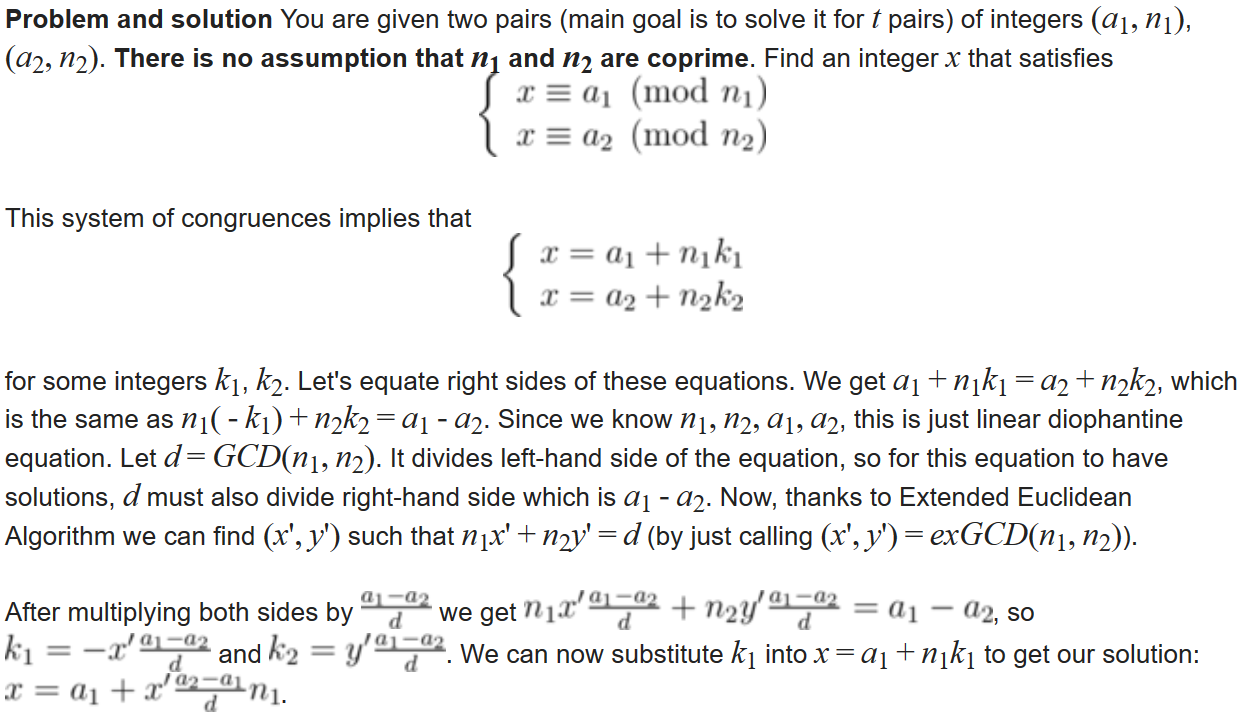
\includegraphics[width=0.5\textwidth,height=0.5\textheight,keepaspectratio]{crt}
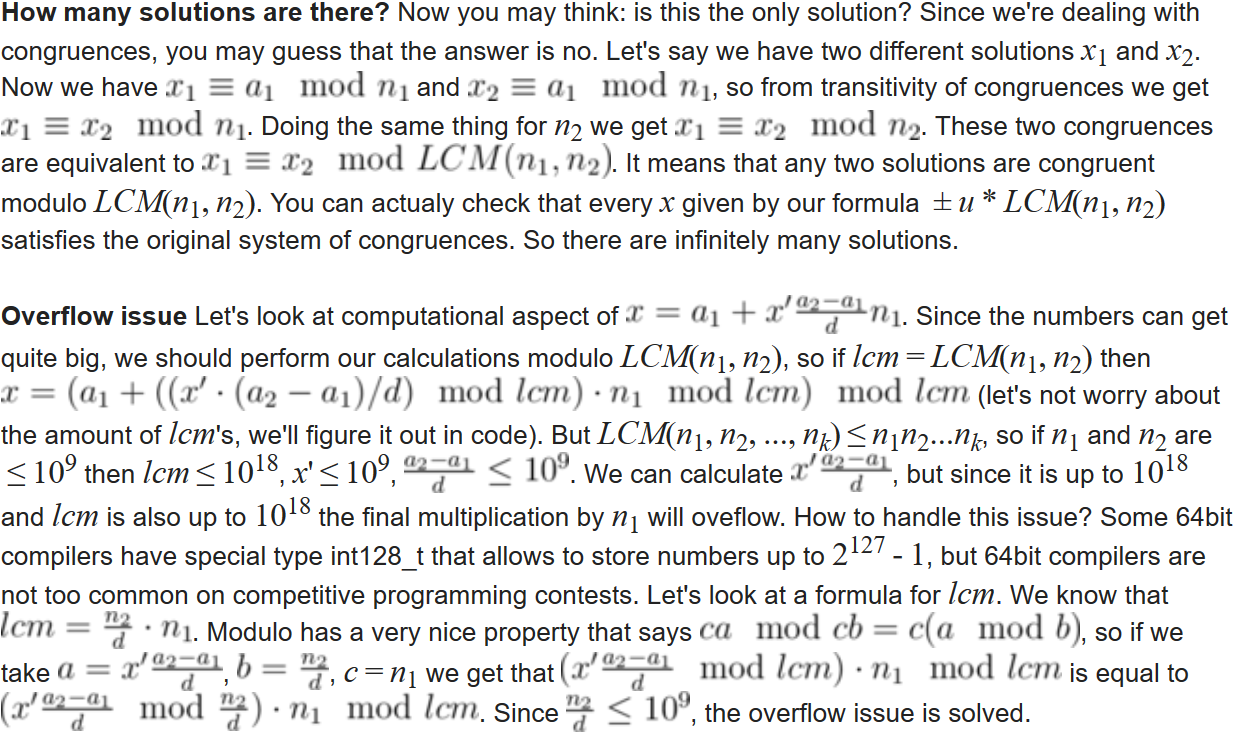
\includegraphics[width=0.5\textwidth,height=0.5\textheight,keepaspectratio]{crt2}
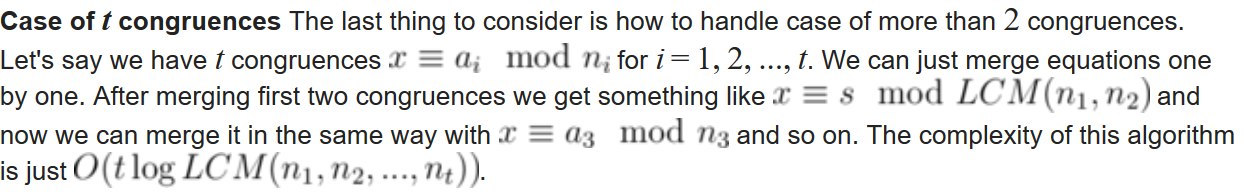
\includegraphics[width=0.5\textwidth,height=0.5\textheight,keepaspectratio]{crt3}
\begin{minted}{cpp}
#include<bits/stdc++.h>
using namespace std;
const int N = 20;
long long GCD(long long a, long long b) { return (b == 0) ? a : GCD(b, a % b); }
inline long long LCM(long long a, long long b) { return a / GCD(a, b) * b; }
inline long long normalize(long long x, long long mod) { x %= mod; if (x < 0) x += mod; return x; }
struct GCD_type { long long x, y, d; };
GCD_type ex_GCD(long long a, long long b)
{
    if (b == 0) return {1, 0, a};
    GCD_type pom = ex_GCD(b, a % b);
    return {pom.y, pom.x - a / b * pom.y, pom.d};
}
int testCases;
int t;
long long a[N], n[N], ans, lcm;
int main()
{
    ios_base::sync_with_stdio(0);
    cin.tie(0);
    cin >> t;
    for(int i = 1; i <= t; i++) cin >> a[i] >> n[i], normalize(a[i], n[i]);
    ans = a[1];
    lcm = n[1];
    for(int i = 2; i <= t; i++)
    {
        auto pom = ex_GCD(lcm, n[i]);
        int x1 = pom.x;
        int d = pom.d;
        if((a[i] - ans) % d != 0) return cerr << "No solutions" << endl, 0;
        ans = normalize(ans + x1 * (a[i] - ans) / d % (n[i] / d) * lcm, lcm * n[i] / d);
        lcm = LCM(lcm, n[i]); // you can save time by replacing above lcm * n[i] /d by lcm = lcm * n[i] / d
    }
    cout << ans << " " << lcm << endl;
 
    return 0;
}
\end{minted}
\href{https://codeforces.com/problemset/problem/687/B}{\textbf{Remainders Game}}\\
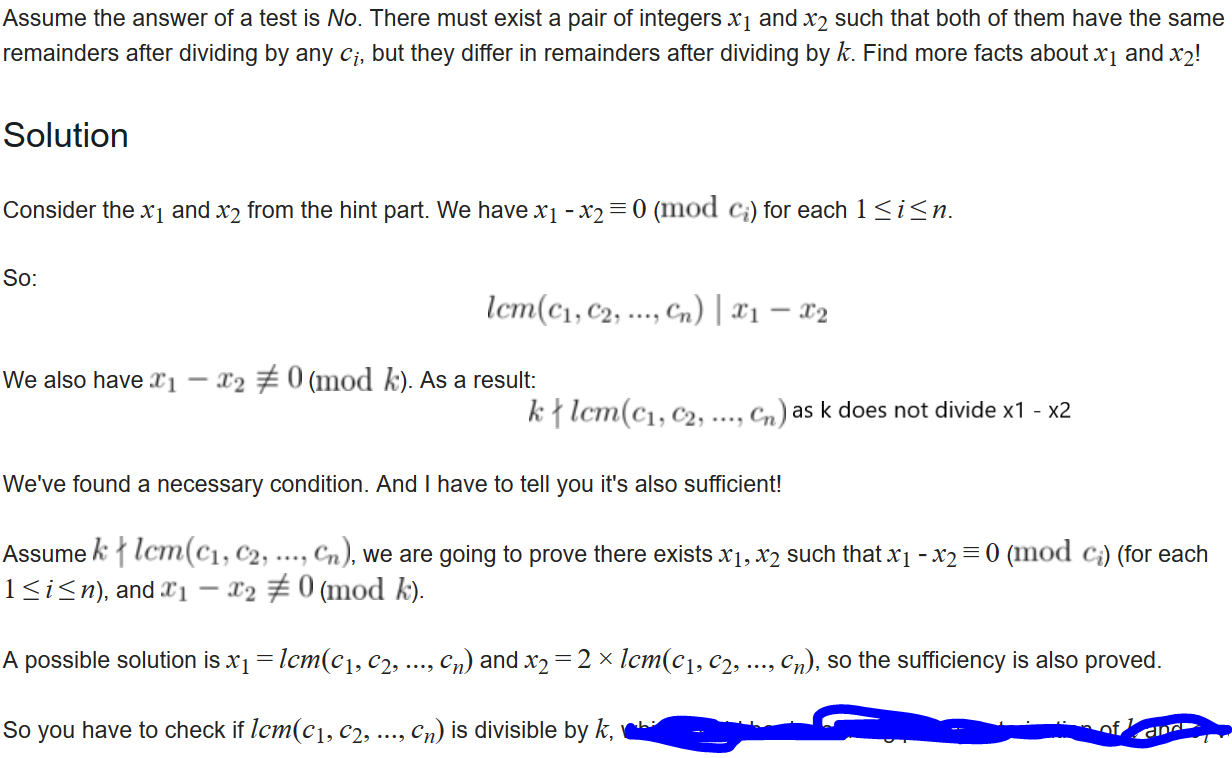
\includegraphics[width=0.5\textwidth,height=0.5\textheight,keepaspectratio]{rem}
\subsection{Primitive Root}
\subsubsection{Definition}

In modular arithmetic, a number $g$ is called a primitive root modulo n if every number coprime to $n$ is congruent to a power of $g$ modulo $n$. Mathematically, $g$ is a primitive root modulo n if and only if for any integer $a$ such that $gcd(a, n) = 1$, there exists an integer $k$ such that:

$g^k \equiv a \pmod n$.

$k$ is then called the index or discrete logarithm of $a$ to the base $g$ modulo $n$. $g$ is also called the generator of the multiplicative group of integers modulo $n$.

In particular, for the case where $n$ is a prime, the powers of primitive root runs through all numbers from $1$ to $n-1$.
\subsubsection{Existence}

Primitive root modulo $n$ exists if and only if:
\begin{itemize}
    \item $n$ is 1, 2, 4, or
    \item $n$ is power of an odd prime number $(n = p^k)$, or
    \item $n$ is twice power of an odd prime number $(n = 2 . p^k)$.
\end{itemize}
This theorem was proved by Gauss in 1801.
\subsubsection{Relation with the Euler function}

Let $g$ be a primitive root modulo $n$. Then we can show that the smallest number $k$ for which $g^k \equiv 1 \pmod n$ is equal $\phi (n)$. Thus gcd (g, n) = 1. Moreover, the reverse is also true, and this fact will be used in this article to find a primitive root.

Furthermore, the number of primitive roots modulo $n$, if there are any, is equal to $\phi (\phi (n) )$.
\subsubsection{Algorithm for finding a primitive root}
From previous section, we know that if the smallest number $k$ for which $g^k \equiv 1 \pmod n$ is $\phi (n)$, then $g$ is a primitive root. Since for any number $a$ relative prime to $n$, we know from Euler's theorem that $a ^ { \phi (n) } \equiv 1 \pmod n$, then to check if $g$ is primitive root, it is enough to check that for all $d$ less than $\phi (n)$, $g^d \not \equiv 1 \pmod n$. However, this algorithm is still too slow. $O(g * \phi (n))$j

From Lagrange's theorem, we know that the index of any number modulo $n$ must be a divisor of $\phi (n)$. Thus, it is sufficient to verify for all proper divisor $d , | , \phi (n)$ that $g^d \not \equiv 1 \pmod n$. This is already a much faster algorithm, but we can still do better.

Factorize $\phi (n) = p_1 ^ {a_1} ... p_s ^ {a_s}$. We prove that in the previous algorithm, it is sufficient to consider only the values of $d$ which has the form $\frac { \phi (n) } {p_j}$. Indeed, let $d$ be any proper divisor of $\phi (n)$. Then, obviously, there exists such $j$ that $d , | , \frac { \phi (n) } {p_j}$, i.e. $d . k = \frac { \phi (n) } {p_j}$. However, if $g^d \equiv 1 \pmod n$, we would get:

$g ^ { \frac { \phi (n)} {p_j} } \equiv g ^ {d . k} \equiv (g^d) ^k \equiv 1^k \equiv 1 \pmod n$.

i.e. among the numbers of the form $\frac {\phi (n)} {p_i}$, there would be at least one such that the conditions are not met.

Now we have a complete algorithm for finding the primitive root:
\begin{itemize}
    \item First, find $\phi (n)$ and factorize it.
    \item Then iterate through all numbers $g = 1 ... n$, and for each number, to check if it is primitive root, we do the following:
        \begin{itemize}
        \item Calculate all $g ^ { \frac {\phi (n)} {p_i}} \pmod n$.
        \item If all the calculated values are different from $1$, then $g$ is a primitive root.
        \end{itemize}
\end{itemize}
Running time of this algorithm is $O(Ans . log \phi (n) . \log n)$ (assume that $\phi (n)$ has $\log \phi (n)$ divisors).

Shoup (1990, 1992) proved, assuming the generalized Riemann hypothesis, that $g$ is $O(log^6 p)$.
\subsubsection{Implementation}

The following code assumes that the modulo p is a prime number. To make it works for any value of p, we must add calculation of $\phi (p)$.
\begin{minted}{cpp}
int generator (int p) {
	vector<int> fact;
	int phi = p-1,  n = phi;
	for (int i=2; i*i<=n; ++i)
		if (n % i == 0) {
			fact.push_back (i);
			while (n % i == 0)
				n /= i;
		}
	if (n > 1)
		fact.push_back (n);
 
	for (int res=2; res<p; ++res) {
		bool ok = true;
		for (size_t i=0; i<fact.size() && ok; ++i)
			ok &= powmod (res, phi / fact[i], p) != 1;
		if (ok)  return res;
	}
	return -1;
}
\end{minted}
\subsection{Discrete Root}

The problem of finding discrete root is defined as follows. Given a prime $n$ and two integers $a$ and $k$, find all $x$ for which:

$x^k \equiv a \pmod n$
\subsubsection{The algorithm}

We will solve this problem by reducing it to the discrete logarithm problem.

Let's apply the concept of a primitive root modulo $n$. Let $g$ be a primitive root modulo $n$. Note that since $n$ is prime, it must exist, and it can be found in $O(Ans \cdot \log \phi (n) \cdot \log n) = O(Ans \cdot \log^2 n)$ plus time of factoring $\phi (n)$.

We can easily discard the case where $a = 0$. In this case, obviously there is only one answer: $x = 0$.

Since we jnow that $n$ is a prime, any number between 1 and $n-1$ can be represented as a power of the primitive root, and we can represent the discrete root problem as follows:

$(g^y)^k \equiv a \pmod n$

where

$x \equiv g^y \pmod n$

This, in turn, can be rewritten as

$(g^k)^y \equiv a \pmod n$

Now we have one unknown $y$, which is a discrete logarithm problem. The solution can be found using Shanks' baby-step-giant-step algorithm in $O(\sqrt {n} \log n)$ (or we can verify that there are no solutions).

Having found one solution $y_0$, one of solutions of discrete root problem will be $x_0 = g^{y_0} \pmod n$.
Finding all solutions from one known solution

To solve the given problem in full, we need to find all solutions knowing one of them: $x_0 = g^{y_0} \pmod n$.

Let's recall the fact that a primitive root always has order of $\phi (n)$, i.e. the smallest power of $g$ which gives 1 is $\phi (n)$. Therefore, if we add the term $\phi (n)$ to the exponential, we still get the same value:

$x^k \equiv g^{ y_0 \cdot k + l \cdot \phi (n)} \equiv a \pmod n \forall l \in Z$

Hence, all the solutions are of the form:

$x = g^{y_0 + \frac {l \cdot \phi (n)}{k}} \pmod n \forall l \in Z$.

where $l$ is chosen such that the fraction must be an integer. For this to be true, the numerator has to be divisible by the least common multiple of $\phi (n)$ and $k$. Remember that least common multiple of two numbers $lcm(a, b) = \frac{a \cdot b}{gcd(a, b)}$; we'll get

$x = g^{y_0 + i \frac {\phi (n)}{gcd(k, \phi (n))}} \pmod n \forall i \in Z$.

This is the final formula for all solutions of discrete root problem.
\subsubsection{Implementation}
\begin{minted}{cpp}
    int delta = phi / gcd (k, phi);
	vector<int> ans;
	for (int cur=any_ans % delta; cur < phi; cur += delta)
		ans.push_back (powmod (g, cur, n));
	sort (ans.begin(), ans.end());
	printf ("%d\n", ans.size());
	for (size_t i=0; i<ans.size(); ++i)
		printf ("%d ", ans[i]);
\end{minted}
\subsection{Fermats last theorem}
No 3 positive integerss a, b, c satisfying the eqn $a^n + b^n = c^n$ for any integer value of n greater than 2.
\subsection{Josephus Problem}
Given natural no. n and k, we write natural nos 1 to n along the circle. Then delete the kth no, (i..e no. k initially) and then from this position next kth no. is deleted and so on.
\\The process stops when there is only one no. remaining, problem asks us to find this no.
\subsubsection{For k = 2}
\begin{eqnarray}n & = & 1, 2, 3, 4, 5, 6\\
f(n) & = & 1, 1, 3, 1, 3, 5
\end{eqnarray}
Thm: if $n = 2^m + l$ where $0 \leq l < 2^m$ then $f(n) = 2l + 1$.
\subsubsection{For general $k \geq 1$}
We should note that after the kth person is killed we are left with a circle of n - 1 and we start the next count with the person whose no in the original problem was $(k \mod n) + 1$. The position of the survivior in the remaining circle would be $f(n - 1, k)$ if we start counting at 1; shifting this to account for the fact that we are starting at $(k \mod n) + 1$ yilds the recurrence $f(n, k) =  ((f(n - 1, k) + k - 1) \mod n) + 1$ with $f(1, k) = 1$ which takes the simpler form $g(n, k) = (g(n - 1, k) + k) \mod n$ with $g(1, k) = 0$. This approach has running time O(n).
\\But for small k and large n, there is another approach. The second apprach alaso uses dp but has running time O(klogn) and is based on cosidering killing kth, 2kth, ..., $(\lfloor n/k \rfloor * k)$th person as one step, then changing the numbering.
\begin{eqnarray}
g(n, k) &=& 0 \text{ if n = 1 (because of 0 indexing)}\\
        &=& (g(n - 1, k) + k) \mod n \text{ if $1 < n < k$}\\
        &=& \lfloor k * ((g(n_m, k) - n \mod k) \mod n_m) / (k - 1) \rfloor \text{ where $n_m = n - \lfloor n/k \rfloor$ if $k \leq n$}
\end{eqnarray}
\subsection{Root Solving}
\begin{minted}{cpp}
// Following is the solution for UVA 10428
#include<bits/stdc++.h>

using namespace std;

typedef long long int ll;
const double eps = 1e-7;
struct Polynomial {
    vector<double> coef;
    int deg;
    Polynomial() {}
    Polynomial(int dd) {
        deg = dd;
        coef.resize(deg + 1);
    }
    void fix(Polynomial &given) {
        int dec = 0;
        for (int i = given.deg; i >= 0; i--) {
            if (abs(given.coef[i]) < eps) {
                dec++;
            } else break;
        }
        dec *= -1;
        given.coef.resize(given.deg + dec + 1);
        given.deg += dec;
        return;
    }
    Polynomial operator + (const Polynomial &other) {
        Polynomial ret;
        if (deg > other.deg) {
            ret.deg = deg;
            ret.coef.resize(deg + 1);
            for (int i = deg; i > other.deg; i--) {
                ret.coef[i] = coef[i];
            }
            for (int i = other.deg; i >= 0; i--) {
                ret.coef[i] = coef[i] + other.coef[i];
            }
            fix(ret);
            return ret;
        } else {
            ret.deg = other.deg;
            ret.coef.resize(other.deg + 1);
            for (int i = other.deg; i > deg; i--) {
                ret.coef[i] = other.coef[i];
            }
            for (int i = deg; i >= 0; i--) {
                ret.coef[i] = coef[i] + other.coef[i];
            }
            fix(ret);
            return ret;
        }
    }
    Polynomial operator - (const Polynomial &other) {
        Polynomial ret;
        if (deg > other.deg) {
            ret.deg = deg;
            ret.coef.resize(deg + 1);
            for (int i = deg; i > other.deg; i--) {
                ret.coef[i] = coef[i];
            }
            for (int i = other.deg; i >= 0; i--) {
                ret.coef[i] = coef[i] - other.coef[i];
            }
            fix(ret);
            return ret;
        } else {
            ret.deg = other.deg;
            ret.coef.resize(other.deg + 1);
            for (int i = other.deg; i > deg; i--) {
                ret.coef[i] = other.coef[i];
            }
            for (int i = deg; i >= 0; i--) {
                ret.coef[i] = coef[i] - other.coef[i];
            }
            fix(ret);
            return ret;
        }
    }
    Polynomial operator * (const pair<double, int> u) {
        double d = u.first;
        int dega = u.second;
        Polynomial ret;
        ret.deg = deg + dega;
        ret.coef.assign(ret.deg + 1, 0);
        for (int i = deg; i >= 0; i--) {
            ret.coef[i + dega] = (coef[i] * d);
        }
        fix(ret);
        return ret;
    }
    bool operator != (const Polynomial &other) {
        if (deg != other.deg) return true;
        for (int i = deg; i >= 0; i--) {
            if (coef[i] != other.coef[i]) return true;
        }
        return false;
    }

};

pair<Polynomial, Polynomial> polyDiv(Polynomial &n, Polynomial &d) { // To do n / d
    Polynomial zero;
    zero.deg = 0;
    zero.coef.push_back(0);
    if (n.deg < d.deg) {
        return make_pair(zero, n);
    }
    Polynomial q;
    q.deg = (n.deg);
    q.coef.assign(q.deg + 1, 0);
    Polynomial r = n;
    while (r != zero and r.deg >= d.deg) {
        double t = (r.coef[r.deg] / d.coef[d.deg]);
        q.coef[r.deg - d.deg] += t;
        r = r - d * make_pair(t, r.deg - d.deg);
    }
    q.fix(q); r.fix(r);
    return make_pair(q, r);
}
double f(Polynomial &a, double x) {
    double result = 0;
    for (int i = a.deg; i >= 0; i--) {
        result = result * x + a.coef[i];
    }
    return result;
}
double f_(Polynomial &a, double x) {
    double result = 0;
    for (int i = a.deg; i > 0; i--) {
        result = result * x + a.coef[i] * i;
    }
    return result;
}
double newtonsMethod(Polynomial &a, double x0) {
    double x1 = x0;
    while (true) {
        x0 = x1;
        x1 = x0 - f(a, x0)/f_(a, x0);
        if (abs(x1 - x0) < eps) break;
    }
    return x1;
}
void findRoot(Polynomial a, vector<double> &roots, int n) {
    for (int i = 0; i < n; i++) {
        roots.push_back(newtonsMethod(a, 0));
        Polynomial d(1);
        d.coef[1] = 1;
        d.coef[0] = -roots.back();
        auto u = polyDiv(a, d);
        a = u.first;
    }
}
int main() {
    ios::sync_with_stdio(false);
    cin.tie(nullptr);
   //  freopen("ina.txt", "r", stdin);
   //  freopen("outa.txt", "w", stdout);
    cout << fixed << setprecision(4);
    int n;
    int caseno = 0;
    while (cin >> n and n) {
        Polynomial a(n);
        caseno++;
        for (int i = n; i >= 0; i--) {
            cin >> a.coef[i];
        }
        cout << "Equation " << caseno << ": ";
        vector<double> roots;
        findRoot(a, roots, n);
        sort(roots.begin(), roots.end());
        cout << roots[0];
        for (int i = 1; i < n; i++) {
            cout << " " << roots[i];
        }
        cout << "\n";
    }
}
\end{minted}
\subsection{Integration}
\subsubsection{Simpson rule}
$$x_i = a + i h, ~~ i = 0 \ldots 2n,$$ $$h = \frac {b-a} {2n}.$$
$$\int_a ^ b f (x) dx \approx \left(f (x_0) + 4 f (x_1) + 2 f (x_2) + 4f(x_3) + 2 f(x_4) + \ldots + 4 f(x_{2N-1}) + f(x_{2N}) \right)\frac {h} {3} $$
\begin{minted}{cpp}
    const int N = 1000 * 1000; // number of steps (already multiplied by 2)

double simpson_integration(double a, double b){
    double h = (b - a) / N;
    double s = f(a) + f(b); // a = x_0 and b = x_2n
    for (int i = 1; i <= N - 1; ++i) { // Refer to final Simpson's formula
        double x = a + h * i;
        s += f(x) * ((i & 1) ? 4 : 2);
    }
    s *= h / 3;
    return s;
}
\end{minted}
\subsection{Side Notes}
\begin{enumerate}
    \item relatively prime is same as coprime.
    \item 2 nos a, b are said to be congruent modulo n, if there difference is an integer multiple of n, i.e. they give same remainder . We denote this as $a \equiv b (\text{mod n})$
    \item For (a, b) three operations exist:
    \begin{enumerate}
        \item If a, b are even then (a/2, b/2).
        \item (a + 1, b + 1)
        \item If (a, b) exist and (b, c) exist then (a, c) exist.
    \end{enumerate}
    Every (x, y) pair s.t. $x < y$ can be transformed to (1, 1 + k x d) where k is any positive integer and d is maximal odd divisor of y - x. We want to generate $(1, a_1), (1, a_2), \dots, (1, a_n)$. So $d | gcd(a_1 - 1, a_2 - 1, \dots, a_n - 1)$. No. of pairs (x, y) which have d as their maximal odd divisors: these are cards with y - x = d, 2d, 4d, 8d, etc. as odd into odd is odd thus we can't multiply with any odd number as it will give bigger odd divisor. Don't forget that numbers x, y must no exceed m. Total no. of cards with some fixed difference t = y - x is exactly m - t. $1 \leq x < y \leq m$\\
    $1 - x \leq 0 < t \leq m - x$\\
    $1 \leq x \leq m - t$\\
    $m - t \geq 1$\\
    $t \leq m - 1$
    \\$2^l * d \leq m - 1$\\
    So sum up $m - 2^l * d$ where d is any odd divisor of gcd($a_1 - 1, \dots$) and l is such that $2^l * d \leq m - 1$.
    \item People in cycle will commit suicide.
    
    \item Every even no. greater than or equal to 4 can be expressed as a sum of 2 prime nos.
    \item No. of digits in a no. $n = \lfloor(\log_{10}{n})\rfloor + 1$
    \item No. of digits in $\binom{n}{k} = \lfloor(\sum_{i = n - k + 1}^{n}\log_{10}{i} - \sum_{i = 1}^{k}\log_{10}{i)})\rfloor + 1$
    \item No. of digits of a no. in some base b$ = floor(1 + \log_b{no.} + eps)$. Also make sure that input no. is not 0.
    \item for $\binom{n}{r}$ always do $r = min (r, n - r)$. Also to compute it either we can use dp or for a specific pair, if it is guarenteed that the final solution lies within data types limit then we can compute it as. \begin{minted}{cpp}
ll ncr(ll n, ll r) {
    r = min (r, n - r);
    ll res = 1;
    for (int k = 1; k <= r; k++, n--) {
        res *= n;
        res /= k;
    }
}
// Another way is
int c[maxn + 5][maxn + 5];
for (int n = 0; n <= maxn; n++) {
    c[n][0] = c[n][n] = 1;
    for (int k = 1; k < n; k++) {
        c[n][k] = c[n - 1][k - 1] + c[n - 1][k];
    }
}
// Or if long arithmetic is allowed, we can do fact[n] / fact[n - k] / fact[k].
    \end{minted}
    \item $(t^a - 1) / (t^b - 1)$ is not an integer with less than 100 digits if t = 1 or $a < b$ or $a \bmod b \neq 0$ or $(a - b) * \log_{10}{t} > 99.0$
    \item \begin{minted}{cpp}
for (int j = 0; j < bigint_var.a.size (); j++) {
    int temp = bigint_var.a[j];
    while (temp > 9) {
        sum += temp % 10;
        temp /= 10;
    }
    sum += temp;
}
    \end{minted}
    \item To get all divisors of a number $n$.
    \begin{minted}{cpp}
for (int i = 1; i * i <= n; i++) {
    if (n % i == 0) {
        d.push_back(i);
        if (i != n / i) d.push_back (n / i);
    }
}
    \end{minted}
    \item We can find the nth root using pow func.
    \item Some times we can generate first few terms and then look up at oeis.org
    \item
\begin{minted}{cpp}
// to compute (a * b) mod m when a * b can go above ll
ll bmodm;
ll compute (ll a, ll &b, ll &m) {
    if (a == 1) return bmodm;
    if (a & 1) return (((2 % m) * compute (a / 2, b, m) + bmodm) % m);
    else return ((2 % m) * compute (a/2, b, m)) % m;
}
\end{minted}
    \item Say $A = [a, b, c, d, e]$ and $P = [4, 3, 2, 0, 1] \rightarrow \text{final array is } [e, d, c, a, b]$. but if we were to get $P^k$ applied to A, we should first represent P by matrix.
    \[\begin{bmatrix}
    0 & 0 & 0 & 1 & 0\\
    0 & 0 & 0 & 0 & 1\\
    0 & 0 & 1 & 0 & 0\\
    0 & 1 & 0 & 0 & 0\\
    1 & 0 & 0 & 0 & 0
    \end{bmatrix}\]
    And then compute it kth power and then do $A * P^k$
\end{enumerate}
\subsection{Important Problems}
\begin{itemize}
	\item \href {https://uva.onlinejudge.org/external/113/11310.pdf}{UVA 11310 Prob}: $dp[n] = dp[n - 1] + 4 * dp[n - 2] + 2 * dp[n - 3]$
	\item \href {https://uva.onlinejudge.org/external/112/11204.pdf}{UVA 11204 Prob}: Tricky problem, it just asks \textit{How many possible arrangements maximizing the assignment of the \textbf{first priority}.} Thus only first priority instrument matters, so if 2 want A, 4 want B, 3 want C, then ans is $2 * 4 * 3$.
    \item \href {https://uva.onlinejudge.org/external/107/10790.pdf}{UVA 10790 Prob}: If there is an intersection that means we have a quadrilateral, hence answer is the number of quadrilaterals $ = \binom{a}{2} * \binom{b}{2}$.
    \item \href {https://uva.onlinejudge.org/external/5/568.pdf}{last non zero digit of fact(n)}, \href {https://gist.github.com/sourabh2311/3e7d2c8c905cce7f04eb86400d4aac35}{Sol}. If you know multiplicatioin limit, take mod with ($10^{\text{no. of digits}}$)
    \item \href {https://uva.onlinejudge.org/external/5/542.pdf}{France 98}, \href {https://gist.github.com/sourabh2311/94629bd0303d3c4f918bda3bdaf8e711}{Sol}.
    \item \href {https://uva.onlinejudge.org/external/100/10061.pdf}{How many zeros and how many digits?} Sol: then iterate through factors of base and get their powers in n!, take min. of all such powers divided by power of prime factor in that base. And for how many digits part, use that log formula.
    \item Is $n!$ divisible by m? Sol: Use prime factors
    \item Given n, maximize (find x) $n - p*x$ where $p*x \leq n < (p + 1)*x$ which somehow happens with $p = 1$
    \item \textbf{Prob: }Lenghts from 1 to n, max. no. of triangles?
            \\\textbf{Sol: }\begin{minted}{cpp}
void precal () {
    F[3] = P[3] = 0;
    ll var = 0;
    for (int i = 4; i <= 1000000; i++) {
        if (i % 2 == 0) {
            var++;
        }
        P[i] = P[i - 1] + var;
        F[i] = F[i - 1] + P[i];
    }
    // F[n] has ans
}
            \end{minted}
    \item Bottom right corner of a chess board must be white. If c == 0/1 bottom right corner of painting is black/white.
    \begin{minted}{cpp}
if (c == 0) ans = (n - 7) * (m - 7) / 2
else ans = ((n - 7) * (m - 7) + 1) / 2
    \end{minted}
    \item for 2 nos (a, b) output 2 nos (c, d) such that a = gcd(c, d) \& b = lcm(c, d) and c is minimum. Sol: basically soln exist if $b \bmod a = 0$ and soln is c = a, d = b.
\end{itemize}
\section{Graphs}
\subsection{Basic}
\begin{itemize}
    \item The shortest path b/w vertices i and j after edge (u, v) is added is equal to $min(d_{i, j}, d_{i, u} + w_{u, v} + d_{v, j}, d_{i, v} + w_{v, u} + d_{u, j})$
    \item In BFS, in case of multiple sources, enqueue them all in queue and set dist[v] = 0. Some trick works in case of dijkstra.
    \item Also in case we are given both source and destination then we can terminate our while loop by checking whether the element we pop from queue is the destination or not. Same trick would work with weighted graph provided we have no -ve edges (dijkstra)
    \item Adjacency matrix equal to its transpose that implies undirected graph.
    \item To check whether the graph is bipartite, we can do bfs and color vertices 0/1.
    \item Graph Check
    \begin{minted}{cpp}
void graphcheck (int u) {
    dfs_num[u] = explored;
    for (auto &v : adjlist[u]) {
        if (dfs_num[v] == unvisited) {  // tree edge
            dfs_parent[v] = u;
            graphcheck (v);
        } else if (dfs_num[v] == explored) {  // back edge hence not DAG.
            if (v == dfs_parent[u]) cout << "two ways\n"
            else cout << "back edge\n"
        } else {  // dfs_num[v] == visited
            // forward/cross edge
            // [u [v v] u] this is tree/forward
            // [v [u u] v] back
            // [v v] [u u] cross
        }

    }
}
    \end{minted}
    \item Getting any cycle
\begin{minted}{cpp}
bool dfs(int v) {
    color[v] = 1;
    for (int u : adj[v]) {
        if (color[u] == 0) {
            parent[u] = v;
            if (dfs(u))
                return true;
        } else if (color[u] == 1) {
            cycle_end = v;
            cycle_start = u;
            return true;
        }
    }
    color[v] = 2;
    return false;
}

void find_cycle() {
    color.assign(n, 0);
    parent.assign(n, -1);
    cycle_start = -1;

    for (int v = 0; v < n; v++) {
        if (dfs(v))
            break;
    }

    if (cycle_start == -1) {
        cout << "Acyclic" << endl;
    } else {
        vector<int> cycle;
        cycle.push_back(cycle_start);
        for (int v = cycle_end; v != cycle_start; v = parent[v])
            cycle.push_back(v);
        cycle.push_back(cycle_start);
        reverse(cycle.begin(), cycle.end());

        cout << "Cycle found: ";
        for (int v : cycle)
            cout << v << " ";
        cout << endl;
    }
}
    \end{minted}
    \item Floodfill
    \begin{minted}{cpp}
int R, C;
string grid[100];
int dr[] = {1, 1, 0, -1, -1, -1, 0, 1};
int dc[] = {0, 1, 1, 1, 0, -1, -1, -1};
int floodfill (int r, int c, char c1, char c2) {
    if (r < 0 || r >= R || c < 0 || c >= C) return 0;
    if (grid[r][c] != c1) return 0;
    int ans = 0;
    grid[r][c] = c2;
    for (int d = 0; d < 8; d++) {
        ans += floodfill (r + dr[d], c + dc[d], c1, c2);
    }
    return ans;
}
    \end{minted}
    \item We can find the number of connected components by simply doing dfs (offline), and online using UFDS.
    \item Highest average is possible only by taking large 
    \item We can use BFS for finding the shortest path in a graph with weights 0 or 1. This required just a little modificatio to normal BFS, if the current edge is of 0 weight and distance to the vertex is shorter than the current found distance, then add this vertex not to the back but to the front of the queue. (we can use dequeue which supports front, back, push\_{}back, push\_{}front, pop\_{}back, pop\_{}front) in O(1).
    \item Find the shortest path of even length from a source vertex s to a target vertex t in an unweighted graph. For this, we must construct an auxiliary graph, whose vertices are the state (v, c) where v is the current node, c = 0, 1 denots the current parity. Any edge (u, v) of the original graph in this new graph will turn into two edges ((u, 0), (v, 1)) and ((u, 1), (v, 0)). After that we run a BFS to find the shortest path from (s, 0) to (t, 0).
    \item Find all the vertices on any shortest path between a given pair of vertices (a, b). To accomplish that, run 2 BFS: one from a and one from b. Let da[] be the array containing shortest distances obtained from first BFS (from a) and db[] be the array containing shortest distances obtained from the second BFS (from b). Now for every vertex it is easy to check whether it lies on any shortest path between a and b: the criterion is the condition da[v] + db[v] = da[b].
    \item Similarly edge (u, v) lies on shortest path if da[u] + 1 + db[v] = da[b].
    \item Finding shortest cycle in a directed unweighted graph. For each vertex $v_i$: do a BFS from it and if we try to gro from the current vertex to an already visited vertex then it means that we have found a cycle and should stop BFS.
    \\Take minimum of all such cycles (one for each $v_i$ to get the shortest length cycle.
    \item Using DFS, we can also tell whether vertex i is an ancestor of j by using either that subtree method or by checking if $entry[i] < entry[j]$ and $exit[i] > exit[j]$
\end{itemize}
\subsection{Articulation Points and Bridges (undirected graph)}
\begin{itemize}
    \item An articulation point is defined as a vertex in a graph G whose removal (all edges incident to this vertex are also removed) disconnects G. A graph without any articulatioin point is called "Biconnected" Similarly, a "Bridge" is defined as an edge in a graph G whose removal disconnects G.
    \begin{minted}{cpp}
        // dfs_low[u] will store the lowest iteration count vertex u can reach from u’s current DFS Tree (i.e u can only reach vertices of lower iteration count only if a back-edge exists in one of its children)
vector<int> dfs_num;
vector<int> dfs_low;
vector<int> dfs_parent;
vector<bool> articulation_vertex;
int dfs_root, root_children;

void ArticulationPoint(int u)
{
    // Initially, dfs_num = dfs_low
    dfs_num[u] = dfs_low[u] = dfs_num_counter++;
    for(int i = 0; i < adj_list[u].size(); i++)
    {
        int v = adj_list[u][i];
        
        // v was not previously visited, i.e a normal tree edge
        if(dfs_num[v] == -1)
        {
            dfs_parent[v] = u;
            
            // special case if u is root
            if(u == dfs_root) root_children++;

            ArticulationPoint(v);
            
            // To detect articulation points
            if(dfs_low[v] >= dfs_num[u])
                articulation_vertex[u] = true;
            // To detect bridges
            if (dfs_low[v.first] > dfs_num[u])
                printf(" Edge (%d, %d) is a bridge\n", u, v.first);
            
            // update dfs_low[u] if dfs_low[v] is lower
            // i.e a back-edge exists in one of u's children
            dfs_low[u] = min(dfs_low[u], dfs_low[v]);
        }
        // if v was previously visited, and v is not the parent of u
        // then a back-edge certainly exists, not a direct cycle
        // update dfs_low[u] to store dfs_num of ancestor is lower than
        // current dfs_low
        else if(v != dfs_parent[u])
            dfs_low[u] = min(dfs_low[u], dfs_num[v]);
    }
}

// Example main usage
int main() 
{
    dfs_num_counter = 0;
    dfs_num.clear(); dfs_num.resize(N, -1);
    dfs_low.clear(); dfs_low.resize(N, 0);
    dfs_parent.clear(); dfs_parent.resize(N, 0);
    articulation_vertex.clear(); articulation_vertex.resize(N, false);

    for(int i = 0; i < N; i++)
        if (dfs_num[i] == -1)
        {
            dfs_root = i; root_children = 0;
            ArticulationPoint(i);
            
            // special case for root
            articulation_vertex[dfs_root] = (root_children > 1);
        }
}
/* Variation

A slight variation to this problem is how many disconnected components would result as a direct consequence of removing a vertex u

Another variation is to find the articulation vertex whose removal would cause a greater amount of components to be disconnected.
General Idea of Variation

Instead of keeping track of whether or not a node is an articulation point using vector<bool> articulation_vertex, we’ll use a vector<int> articulation_vertex to keep track of how many components will be connected after the removal of vertex u.

To achieve this, we’ll first assume that each node in our graph G is not an articulation vertex. In other words, the removal of any node u in G will result in there being only one connected component (G will remain one entity and not be disconnected).

We’ll then use the same algorithm we’ve used before, however, this around around, whenever we find that u is an articulation vertex relative to one of its children, we’ll increment articulation_vertex[u].

So, if we have a vertex u with say, 3 child components with no back-edges, the removal of u will result in G being cut into four connected components.
*/
vector<int> dfs_num;
vector<int> dfs_low;
vector<int> dfs_parent;
int dfs_root, root_children;


// vector<int> instead of vector<bool>
vector<int> articulation_vertex;

void ArticulationPoint(int u)
{
    dfs_num[u] = dfs_low[u] = dfs_num_counter++;
    for(int i = 0; i < adj_list[u].size(); i++)
    {
        int v = adj_list[u][i];
        
        if(dfs_num[v] == -1)
        {
            dfs_parent[v] = u;
            if(u == dfs_root) root_children++;

            ArticulationPoint(v);
            
            // we increment articulation_vertex here
            if(dfs_low[v] >= dfs_num[u])
                articulation_vertex[u]++;
            if (dfs_low[v.first] > dfs_num[u])
                printf(" Edge (%d, %d) is a bridge\n", u, v.first);
                
            dfs_low[u] = min(dfs_low[u], dfs_low[v]);
        }
        else if(v != dfs_parent[u])
            dfs_low[u] = min(dfs_low[u], dfs_num[v]);
    }
}

int main() 
{
    dfs_num_counter = 0;
    dfs_num.clear(); dfs_num.resize(N, -1);
    dfs_low.clear(); dfs_low.resize(N, 0);
    dfs_parent.clear(); dfs_parent.resize(N, 0);
    
    // articulation_vertex initialized to 1 here
    articulation_vertex.clear(); articulation_vertex.resize(N, 1);

    for(int i = 0; i < N; i++)
        if (dfs_num[i] == -1)
        {
            dfs_root = i; root_children = 0;
            ArticulationPoint(i);
            
            // special case for root
            // number of connected components after the removal of root
            // is equal to how many children root has
            articulation_vertex[dfs_root] = root_children;
        }
}
    \end{minted}
    \item \href{https://gist.github.com/sourabh2311/01c2bdf3f7389c2b84d40db5cce506f9}{Two way to one way UVA 610}
\end{itemize}
\subsection{Tree}
Undirected, acyclic, connected, $|V| - 1$ edges.\\
All edges are bridges, and internal vertices (degree $> 1$) are articulation points.\\
It is as well a bipartite graph.\\
\textbf{SSSP}: Simply take the sum of edge weights of that unique path. $O(|V|)$\\
\textbf{APSP}: Simply do SSSP from all vertices. $O(|V^2|)$
\begin{minted}{cpp}
void preorder (v) {
	visit (v);
	preorder (left (v));
	preorder (right (v));
}
void inorder (v) {
	inorder (left (v));
	visit (v);
	inorder (right (v));
}
void postorder (v) {
	postorder (left (v));
	postorder (right (v));
	visit (v);
}
\end{minted}
It is \textbf {impossible} to construct binary tree with just Preorder traversal.\\ 
It is \textbf {impossible} to construct binary tree with just Inorder traversal.\\
It is \textbf {impossible} to construct binary tree with just Postorder traversal.
\subsubsection{LCA}
\begin{itemize}
    \item \href {https://codeforces.com/contest/916/problem/E}{Jammie and Tree}, \href {https://github.com/sourabh2311/Competitive-Programming/blob/master/CF/457D2/E.cpp}{Sol}: One stop soln to understand LCA. Note that LCA of two nodes u, v is the node w that is ancestor of both u and v and that has the greatest depth in the tree.\\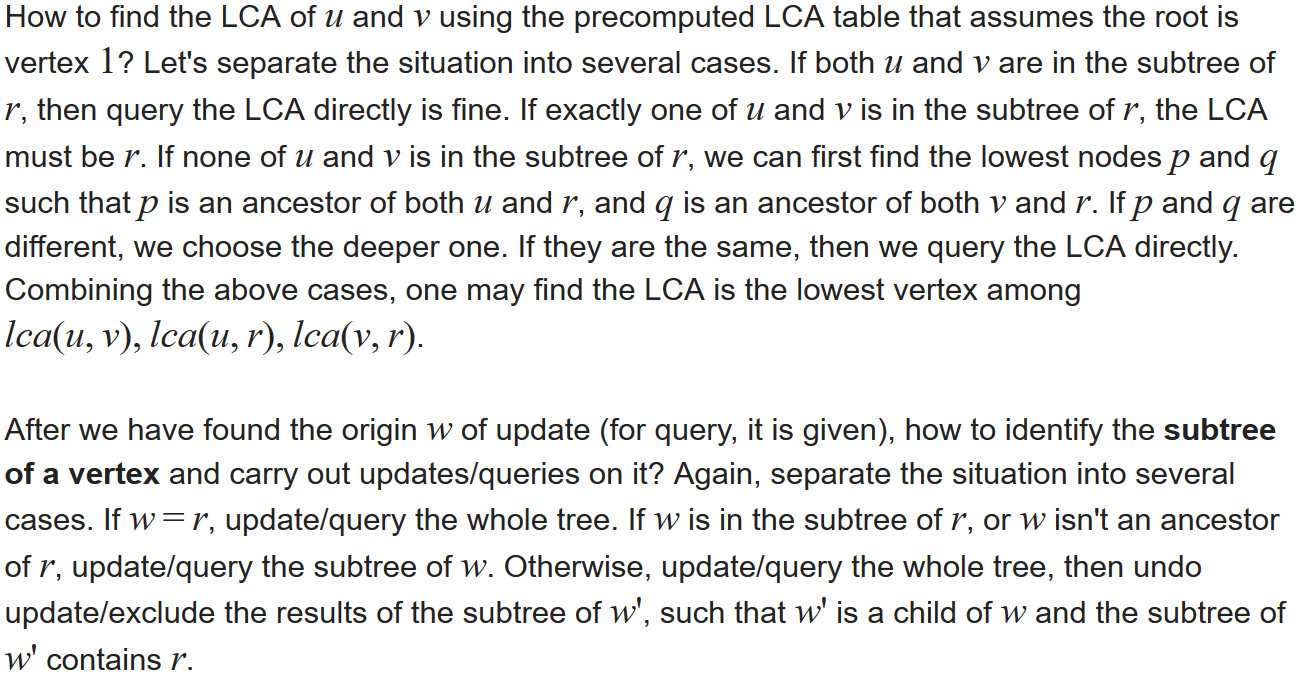
\includegraphics[width=0.5\textwidth,height=0.5\textheight,keepaspectratio]{lca}
    \item Tarjan's offline LCA. for each query (a, b) you should do q[a].pb(b) and q[b].pb(a).
\\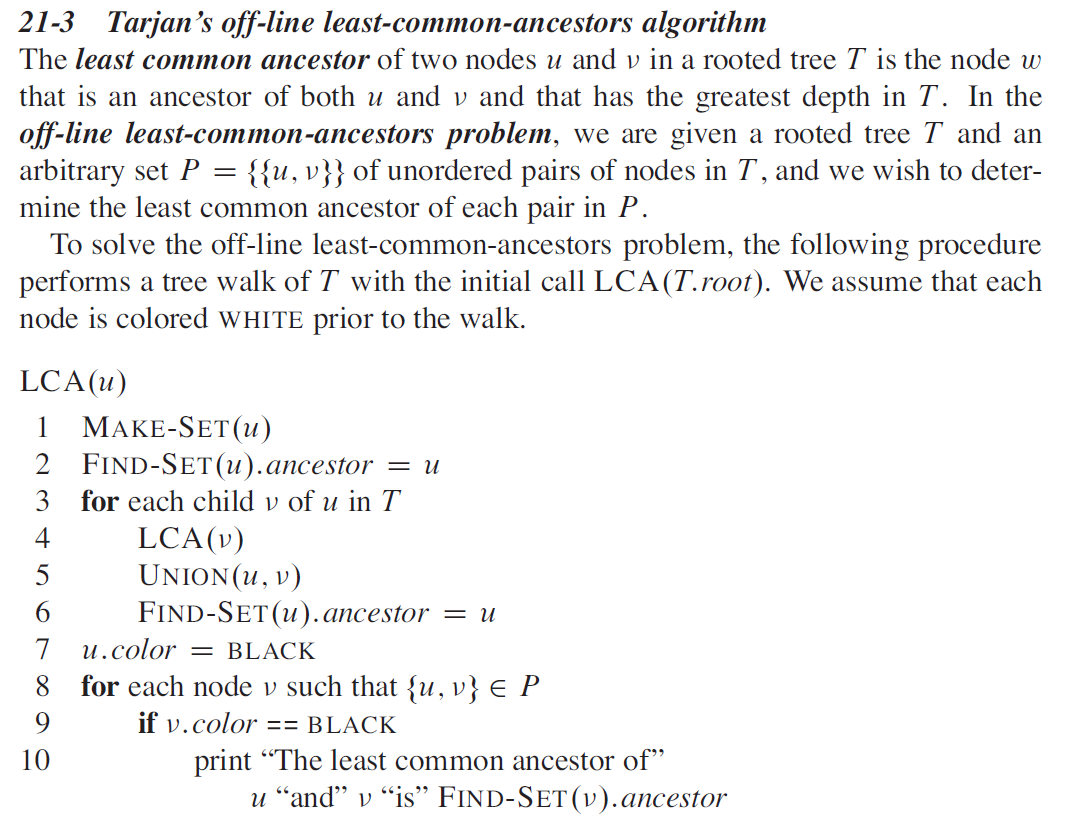
\includegraphics[width=0.5\textwidth,height=0.5\textheight,keepaspectratio]{tar}
\end{itemize}
\subsubsection{Important Problems}
\begin{itemize}
	\item \href {https://gist.github.com/sourabh2311/6cff69fef833097556696bd6f31f3f1d}{UVA 11695 Sol}: Problem Desc: Find which edge to remove and add so as to minimise the number of hops to travel between flights.\\
	Problem Sol: Just link the center of diameters. Brute force which edge to remove. 
	\item \href {https://github.com/sourabh2311/Competitive-Programming/blob/master/UVA_112.cpp}{UVA 112 Sol}, \href {https://uva.onlinejudge.org/external/1/112.pdf}{UVA 112 Prob}: Just see how I processed the input.	
	\item \href {https://gist.github.com/sourabh2311/6b761c14bef4e5887e6b03b809bc4983}{UVA 10029 Sol}, \href {https://uva.onlinejudge.org/external/100/10029.pdf}{UVA 10029 Prob}: Edit steps, (lexicographic sequence of words)	
	\item \href {https://gist.github.com/sourabh2311/d73572fab5cf6d390f509d29abf4cd60}{UVA 536 Sol}, \href {https://uva.onlinejudge.org/external/5/536.pdf}{UVA 536 Prob}: Construct binary tree with preorder and inorder	
	\item \href {https://gist.github.com/sourabh2311/25edb7a7067948832ade9192bd2635ce}{UVA 10459 Sol}, \href {https://uva.onlinejudge.org/external/104/10459.pdf}{UVA 10459 Prob}: Centers of diameters are best where as corners are worst.	
    \item \href{https://codeforces.com/contest/911/problem/F}{Tree Destruction}, \href{https://codeforces.com/contest/911/submission/34122817}{Sol}:
    \item \href{https://codeforces.com/contest/1092/problem/F}{Tree with maximum cost}, \href{https://github.com/sourabh2311/Competitive-Programming/blob/master/CF/527%20Div3/F.cpp}{sol}
\end{itemize}
\subsubsection{MVC on Tree}
\begin{minted}{cpp}
int mvc(int at, int flag, int parent) { //You can start this from any node, i.e. in main: int ans =  min(mvc(0, 0, -1), mvc(0, 1, -1)); and handle the case n == 1 seperately
   if(memo[at][flag] != -1) {
       return memo[at][flag];
   }
   if(glist[at].size() == 1 and parent != -1) { //leaf node
       return memo[at][flag] = flag;
   }
   int ans = flag;
   if(flag) // to take this
   {
       for(auto to : glist[at]) {
           if(to != parent)
               ans += min(mvc(to, 0, at), mvc(to, 1, at));
       }
   } else { //we must take its neighbours
       for(auto to : glist[at]) {
           if(to != parent)
               ans += mvc(to, 1, at);
       }
   }
   return memo[at][flag] = ans;
}  // Similar code can be written to find MWIS.
\end{minted}
\subsubsection{MWIS on Tree}
\begin{minted}{cpp}
int mwis(int at, int flag, int parent) { //You can start this from any node, i.e. in main: int ans =  max(mwis(0, 0, -1), mwis(0, 1, -1)); and handle the case n == 1 seperately
   if(memo[at][flag] != -1) {
       return memo[at][flag];
   }
   if(glist[at].size() == 1 and parent != -1) { //leaf node
        flag ? ans = weight[at] : 0;
        return ans;
   }
   if (flag) {
       ans = weight[v];
       for (auto to : glist[at]) {
           if (to != parent)
            ans += mwis (to, 0, at);
       }
   } else {
        ans = 0;
        for (auto &to : glist[at]) {
            ans += max (mwic(to, 1, at), mwic(to, 0, at));
        }
   }
   return memo[at][flag] = ans;
}  // Similar code can be written to find MWIS.
\end{minted}
\subsection{Terminology}
\begin{itemize}
    \item A \textbf{vertex cover} is a subset of vertices S, such that for each edge (u, v) in graph, either u or v (or both) are in S.
    \item An \textbf{independent set} is a subset of vertices S, such that no two vertices u, v in S are adjacent in graph.
    \item A subset of vertices is a vertex cover iff the complement of the set is an independent set. I.e. $MinVC + MaxIS = V$.
    \item It is easy to see why it is the case, firstly for vertices in the complement of MinVC, they can't have any edge between them as then our MinVC isnt VC. Also if we add to this IS any more vertex then it wont be an IS. Suppost it is not the maximum then there occurs an MIS with size more than this, clearly its complement is VC which would have size smaller than our MinVC which leads to contradiction. 
    \item Complement of VC is an IS and vice versa (easy to see)
    \item Given an undirected graph G = (V, E) and weighting function defined on the vertex set, the minimum weighted vertex cover problem is to find a vertex set S ⊆ V whose total weight is minimum subject to every edge of G has at least one end point in S. 
    \item In the maximum-weight independent set problem, the input is an undirected graph with weights on its vertices and the output is an independent set with maximum total weight.
    \item Again it happens to be the case that size of MWVC + MWIS = Total weight = V.
    \item A matching is a subset of edges such that each vertex is adjacent to at most one edge in the subset. Clearly Matching edges can be atmost $|V|/2$ as each edge joins two vertices and now no other matched edge can touch them.
    \item Note: This MVC, MIS, MM, is defined for undirected, unweighted graph.
    \item Once we have maximum matching. Clearly since these matching edges are aswell edges of the graph and minimum vertex cover should have vertices that are adjacent to these edges. But since matching edges have no vertex in common, size of minimum vertex cover is atleast the size of maximum matching.
    \item Maximum matchings can be found in polynomial time for any graph, while minimum vertex cover is NP complete. Thus, finding maximum independent sets is another NP-complete problem.
    \item The equivalence between matching and covering articulated in Kőnig's theorem allows minimum vertex covers and maximum independent sets to be computed in polynomial time for bipartite graphs, despite the NP-completeness of these problems for more general graph families.
\end{itemize}
\subsection{Konigs Theorem}
Size of Min VC in a bipartite graph is equal to the size of Max Matching in that graph.
\\Kőnig's theorem can be proven in a way that provides additional useful information beyond just its truth: the proof provides a way of constructing a minimum vertex cover from a maximum matching.
\\\textbf{Proof: } Let $G = (V, E)$ be a bipartite graph, and let the vertex set $V$ V be partitioned into left set $L$ and right set $R$. Suppose that $M$ is a maximum matching for $G$.
\\let $U$ be the set of unmatched vertices in $L$ (possibly empty), and let $Z$ be the set of vertices that are either in $U$ or are connected to $U$ by alternating paths. Let $K = ( L \setminus Z ) \cup ( R \cap Z )$. 
\\Every edge $e$ in $E$ either belongs to an alternating path (and has a right endpoint in $K$, or it has a left endpoint in $K$. For, if $e$ is matched but not in an alternating path, then its left endpoint cannot be in an alternating path (for such a path would have had to have included $e$) and thus belongs to $L \setminus Z$. Alternatively, if $e$ is unmatched but not in an alternating path, then its left endpoint cannot be in an alternating path, for such a path could be extended by adding $e$ to it. Thus, $K$ forms a vertex cover.\\
Additionally, every vertex in $K$ is an endpoint of a matched edge. For, every vertex in $L \setminus Z$ is matched because $Z$ is a superset of $U$. And every vertex in $R \cap Z$ must also be matched, for if there existed an alternating path to an unmatched vertex then changing the matching by removing the matched edges from this path and adding the unmatched edges in their place would increase the size of the matching. However, no matched edge can have both of its endpoints in $K$. Thus, $K$ is a vertex cover of cardinality equal to $M$, and must be a minimum vertex cover.
\\Small diagram to understand proof well.
\definecolor{myblue}{RGB}{80,80,160}
\definecolor{mygreen}{RGB}{80,160,80}

\begin{tikzpicture}[thick,
  every node/.style={draw,circle},
  fsnode/.style={fill=myblue},
  ssnode/.style={fill=mygreen},
  every fit/.style={ellipse,draw,inner sep=-2pt,text width=2cm},
  ->,shorten >= 3pt,shorten <= 3pt
]

% the vertices of U
\begin{scope}[start chain=going below,node distance=7mm]
\foreach \i in {1,2, 3}
  \node[fsnode,on chain] (f\i) [label=left: \i] {};
\end{scope}

% the vertices of V
\begin{scope}[xshift=4cm,yshift=-0.5cm,start chain=going below,node distance=7mm]
\foreach \i in {4, 5}
  \node[ssnode,on chain] (s\i) [label=right: \i] {};
\end{scope}

% the set U
\node [myblue,fit=(f1) (f3),label=above:$U$] {};
% the set V
\node [mygreen,fit=(s4) (s5),label=above:$V$] {};

% the edges
\draw (f1) -- (s5);
\draw (f2) -- (s4);
\draw (f3) -- (s5);
\end{tikzpicture}
\\Matched edges are (2, 4) and (3, 5).\\
$U = \{1\}$, 
$Z = \{1, 5, 3\}$, 
$L = \{1, 2, 3\}$, 
$K = \{2, 5\}$
\subsection{Bipartite Matching}
\subsubsection{Hopcroft Karp}
\begin{enumerate}
    \item \textbf{Free node or vertex: }Given a matching M, a node that is not a part of mathing is called a free node. Initially all vertices are free.
    \item \textbf{Matching and not matching edges: }Given a matching M, edges that are part of matching are called matching edges and edges that are not part of M (or connect free nodes) are called non matching edges.
    \item \textbf{Alternating Paths: }Given a matching M, an alternating path is a path in which edges belong alternatively to the matching and not matching.
    \item \textbf{Augmenting path: }Given a matching M, an augmenting path is an alternating path that starts from and ends on free vertices.
    \item The Hopcroft karp algorithm is based on below concept:
    \item A matching M is not maximum if there exist an augmenting path. It is also true other way, i.e., a matching is maximum if no augmenting path exists.
    \item Hopcroft Karp Algo $O(\sqrt{V}*E)$: 
    \begin{enumerate}
        \item Initialize maximal matching M as empty.
        \item While there exists an augmenting path P, remove matching edges of P from M and add not matching edges of P to M. (This increases size of M by 1 as P starts and ends with a free vertex).
        \item Return M.
    \end{enumerate}
The following is the sol to problem \href {https://uva.onlinejudge.org/external/114/11419.pdf}{UVA 11419} where we were just required to find minimum vertex cover.
    \begin{minted}{cpp}
#include <bits/stdc++.h>
#define FOR(i, a, b) for (int i = a; i <= b; i++)
#define REP(i, n) for (int i = 0; i < n; i++)
#define pb push_back
#define INF 500000000
#define maxN 1010
using namespace std;

int n, m, matchX[maxN], matchY[maxN];
int dist[maxN];
vector<int> adj[maxN];
bool Free[maxN];

bool bfs() {
    queue<int> Q;
    FOR (i, 1, n)
        if (!matchX[i]) {  // only free vertices are pushed in queue and have their distance set to 0. Thus already matched vertices in X will have their distance set to INF.
            dist[i] = 0;
            Q.push(i);
        }
        else dist[i] = INF;
    dist[0] = INF;  // 0 is nil
    // Thus we would always start from free vertices traverse then alternating path and if in end from Y there is no match i.e. its a free vertice, we found an augmenting path.
    // Side Notes: If we popped an already matched vertex from queue then it wont go to its matching edges neighbor as its matchY is popped vertex itself and hence it wont have distance set to INF.
    while (!Q.empty()) {
        int i = Q.front(); Q.pop();
        REP(k, adj[i].size()) {
            int j = adj[i][k];
            if (dist[matchY[j]] == INF) {
                dist[matchY[j]] = dist[i] + 1;
                Q.push(matchY[j]);
            }
        }
    }
    return dist[0] != INF;
}

bool dfs(int i) {
    if (!i) return true; // to handle nil.
    REP(k, adj[i].size()) {
        int j = adj[i][k];
        if (dist[matchY[j]] == dist[i] + 1 && dfs(matchY[j])) {
            matchX[i] = j;
            matchY[j] = i;
            return true;
        }
    }
    dist[i] = INF;
    return false;
}

int hopcroft_karp() {
    int matching = 0;
    while (bfs())
        FOR (i, 1, n)
            if (!matchX[i] && dfs(i))
                matching++;
    return matching;
}

void dfs_konig(int i) {
    Free[i] = false;
    REP(k, adj[i].size()) {
        int j = adj[i][k];
        if (matchY[j] && matchY[j] != INF) {
            int x = matchY[j];
            matchY[j] = INF;  // as we have undirected edge, we dont want to traverse that same edge again, so its just a way of noting that.
            if (Free[x]) dfs_konig(x);
        }
    }
}

void solve() {
    printf("%d", hopcroft_karp());
    FOR (i, 1, n)
        if (!matchX[i])
            dfs_konig(i);  // finding Z.
    FOR (i, 1, n)
        if (matchX[i] && Free[i])  // i.e. in L but not in Z.
            printf(" r%d", i);
    FOR (j, 1, m)
        if (matchY[j] == INF)  // i.e. we traversed this edge i.e. its in R intersection Z.
            printf(" c%d", j);
    putchar('\n');
}

void initialize() {
    FOR (i, 1, n) {
        adj[i].clear();
        matchX[i] = 0;
        Free[i] = true;
    }
    memset(matchY, 0, (m + 1) * sizeof(int));
}

int ar[5];
char buff[20];
void read_line() {
    gets(buff);
    int len = strlen(buff), i = 0, m = 0;
    while (i < len)
        if (buff[i] != ' ') {
            ar[m] = 0;
            while (i < len && buff[i] != ' ')
                ar[m] = ar[m] * 10 + buff[i++] - 48;
            m++;
        }
        else i++;
}

main() {
    int k, u, v;
    while (scanf(" %d %d %d ", &n, &m, &k) != EOF) {
        if (!n && !m && !k) break;
        initialize();
        while (k--) {
            read_line();
            adj[ar[0]].pb(ar[1]);
        }
        solve();
    }
}
    \end{minted}
\end{enumerate}
\subsubsection{Using max flow algo}
Our MM problem can be reduced to max flow problem by assigning a dummy source vertex s connected to all vertices in set 1 and all vertices in set 2 are connected to dummy sink vertex t. The edges are directed (s to u, u to v, v to t) where u belongs to set 1 and v belongs to set 2). By setting capacities of all edges in this flow graph to 1, we satisfy the criteria of matching. Thus, this max flow will be equal to the max. no. of matchings on the original graph.

\subsection{Paths}
\begin{itemize}
    \item An \textbf{euler path} is defined as a path in a graph which visits each edge of the graph exactly once. Similarly and \textbf{euler tour/cycle }is an euler path which starts \& ends on the same vertex. A graph which has either an euler path or an euler tour is called \textbf{eulerian}.
    \item For $undirected graph$ euler tour exist $iff$ all vertices have even deg.
    \item For $undirected graph$ euler path exists $iff$ all except 2 vertices have even deg. This euler path will start from one of thee odd deg vertices and end in the other.
    \item For $directed graph$, euler tour exists $iff$ every verte has equal indeg \& outdeg.
    \item For $directed graph$, euler path exists $iff$ at most one vertex has $(outdeg) - (indeg) = 1$, atmost one vertex has $(indeg) - (outdeg) = 1$, every other vertex has $indeg = outdeg$.
\end{itemize}
\begin{minted}{cpp}
// Code to find euler tour (will be able to euler path provided we start with correct vertex) for an undirected graph.
list<int> cyc; // we need list for fast insertion in the middle
void EulerTour(list<int>::iterator i, int u) {
    for (int j = 0; j < (int)AdjList[u].size(); j++) {
        ii v = AdjList[u][j];
        if (v.second) { // if this edge can still be used/not removed
            v.second = 0; // make the weight of this edge to be 0 (‘removed’)
            for (int k = 0; k < (int)AdjList[v.first].size(); k++) {
                ii uu = AdjList[v.first][k]; // remove bi-directional edge
                if (uu.first == u && uu.second) {
                    uu.second = 0;
                    break;
                } 
            }
            EulerTour(cyc.insert(i, u), v.first);
        } 
    }
}
// inside int main()
cyc.clear();
EulerTour(cyc.begin(), A); // cyc contains an Euler tour starting at A
for (list<int>::iterator it = cyc.begin(); it != cyc.end(); it++)
    printf("%d\n", *it); // the Euler tour
\end{minted}
\subsubsection{No. of paths}
\begin{itemize}
    \item No. of paths of length L, from a to b is stored in $M^L[a][b]$. Note that the graph is directed and unweighted, basically $m_{i, j} = 1$ if there is an edge from i to j. This would work even in case of multiple edges if some pair of vertices (i, j) is connected with m edges then we can record this in the adjacency matrix by setting M[i][j] = m. Also this would work if the graph contains loops (a loop is an edge that connects a vertex with itself).\\Proof of this algo: $C_{k + 1}[i][j] = \sum_{p = 1}^nC_k[i][p]\cdot G[p][j]$
    \item No. of shortest paths of fixed length: We are given a directed weighted graph G, G[i][j] = weight of an edge (i, j) and is equal to infinity if there is no edge for each pair of vertices (i, j) we have to find the length of the shortest path between i and j that consists of exactly k edges. $$L_{k + 1}[i][j] = min_{p = 1, \dots, n}(L_k[i][p] + G[p][j])$$
    i.e. $L_{k + 1} = L_k \odot G$ where $A \odot B = C \Leftrightarrow C_{i, j} = min_{p = 1, \dots, n}(A_{i, p} + B_{p, j})$.\\$L_k = G^{\odot k}$. Note that n is the number of vertices.
    \item The above two solns were for fixed k. However the solns can be adapted for solving problems for which the paths are allowed to contain no more than k edges. This can be done by slightly modifying the input graph. We duplicate each vertex: for each vertex v, we create one more vertex $\hat{v}$ and add edge (v, $\hat{v}$) and the loop ($\hat{v}, \hat{v}$). The no. of paths between i and j with atmost k edges is the same no. as the no. of paths between i and $\hat{j}$ with exactly $k + 1$ edges since there is a bijection that maps every path [$p_0 = i, p_1, \dots, p_{m - 1}, p_m = j$] of length $m \leq k$ to the path [$p_0 = i, p_1, \dots, p_{m - 1}, p_m = j, \hat{j}, \dots, \hat{j}$] of length $k + 1$.
    \\ The same trick can be applied to compute the shortest paths with atmost k edges. We again duplicate each vertex and add 2 mentioned edges with weight 0. 
\end{itemize}

\subsection{SCC}
Strongly Connected Components. A directed graph is strongly connected if there is a path between all pairs of vertices. A strongly connected component (SCC) of a directed graph is a maximal strongly connected subgraph
\subsubsection{Tarjan}
\begin{minted}{cpp}
vi dfs_num, dfs_low, S, visited; // global variables
void tarjanSCC(int u) {
    dfs_low[u] = dfs_num[u] = dfsNumberCounter++; // dfs_low[u] <= dfs_num[u]
    S.push_back(u); // stores u in a vector based on order of visitation
    visited[u] = 1;
    for (int j = 0; j < (int)AdjList[u].size(); j++) {
        ii v = AdjList[u][j];
        if (dfs_num[v.first] == UNVISITED)
            tarjanSCC(v.first);
        if (visited[v.first]) // condition for update
            dfs_low[u] = min(dfs_low[u], dfs_low[v.first]); 
    }
    if (dfs_low[u] == dfs_num[u]) { // if this is a root (start) of an SCC
        printf("SCC %d:", ++numSCC); // this part is done after recursion
        while (1) {
            int v = S.back(); S.pop_back(); visited[v] = 0;
            printf(" %d", v);
            if (u == v) break; 
        }
        printf("\n");
    } 
}
// inside int main()
dfs_num.assign(V, UNVISITED); dfs_low.assign(V, 0); visited.assign(V, 0);
dfsNumberCounter = numSCC = 0;
for (int i = 0; i < V; i++)
    if (dfs_num[i] == UNVISITED)
        tarjanSCC(i);
\end{minted}
\subsubsection{Kosaraju}
\begin{enumerate}
    \item It is obvious that strongly connected components do not intersect each other, i.e. this is a partition of all graph vertices. Thus we can give a definition of condensation graph $G^{SCC}$ as a graph containing every strongly connected component as one vertex. Each vertex of the condensation graph corresponds to the strongly connected component of the graph $G$. There is a direccted edge b/w two vertice $C_i$ and $C_j$ of the condensation graph iff there are 2 vertices $u \in C_i$ and $v \in C_j$ such that there is an edge in initial graph, i.e. $(u, v) \in E$. The most important property of the condensation grph is that it is acyclic.
    \item Let $C \& C^`$ be 2 diff SCC \& there is an edge $(C, C^`)$ in a condensation graph then $tout[C] > tout[C^`]$, note: $tout[C] = max_{v_i \in C}(tout[v_i])$.
\end{enumerate}
\begin{minted}{cpp}
vector < vector<int> > g, gr;
vector<bool> used;
vector<int> order, component;

void dfs1 (int v) {
    used[v] = true;
    for (size_t i=0; i<g[v].size(); ++i)
        if (!used[ g[v][i] ])
            dfs1 (g[v][i]);
    order.push_back (v);
}

void dfs2 (int v) {
    used[v] = true;
    component.push_back (v);
    for (size_t i=0; i<gr[v].size(); ++i)
        if (!used[ gr[v][i] ])
            dfs2 (gr[v][i]);
}

int main() {
    int n;
    ... reading n ...
    for (;;) {
        int a, b;
        ... reading next edge (a,b) ...
        g[a].push_back (b);
        gr[b].push_back (a);
    }

    used.assign (n, false);
    for (int i=0; i<n; ++i)
        if (!used[i])
            dfs1 (i);
    used.assign (n, false);
    for (int i=0; i<n; ++i) {
        int v = order[n-1-i];
        if (!used[v]) {
            dfs2 (v);
            ... printing next component ...
            component.clear();
        }
    }
}
\end{minted}
\subsection{SAT}
\subsubsection{1 SAT}
$f = x_1 \wedge x_2 \wedge \dots \wedge x_n$ is satisfiable iff there isnt both $x_i \& \bar{x_i}$ in $f$.
\subsubsection{2 SAT}
$f = (x_1 \vee y_1) \wedge \dots \wedge (x_n \vee y_n)$ is satisfiable iff both $x_i \& \bar{x_i}$ are not in same SCC as one them has to be true and in SCC one value is true all others must be true. For each $(x_i \vee y_i)$ add 2 edges $\bar{x_i} \rightarrow y_i$ and $\bar{y_i} \rightarrow x_i$. 
\\After seeing whether the soln exists or not, soln can be constructed with the help of Kosaraju's algo, let comp[v] denote the index of strongly connected component to which the vertex v belongs. Then, if $comp[x] < comp[\bar{x}]$ we assign x with false and true otherwise.
\subsection{DAG}
topological sort or topological ordering of a directed graph is a linear ordering of its vertices such that for every directed edge uv from vertex u to vertex v, u comes before v in the ordering.
\\A topological ordering is possible if and only if the graph has no directed cycles, that is, if it is a directed acyclic graph (DAG). Any DAG has at least one topological ordering.
\begin{minted}{cpp}
void dfs (int from) {
    visited[from] = true;
    for (int i = 0; i < adjlist[from].size (); i++) {
        if (!visited[adjlist[from][i]]) dfs (adjlist[from][i]);
    }
    ts.pb (from); 
}
// in main
for (int i = 0; i  < V; i++) {
    if (!visited[i]) {
        dfs(i);
    }
}
reverse (ts.begin (), ts.end ());
\end{minted}
\subsubsection{SSSP}
Do topological sort then relax edges according to this order.
\subsubsection{SSLP}
Simply negate all the edge weights and run SSSP as above.
\\Pay attention on the word "we are not allowed to go back" so dont use normal SSSP algo but relax edges according to the required order.
\subsubsection{Counting Paths in DAG}
find toposort. Set numPaths[firstElement] = 1. Then we process the remaining vertices one by one acc. to toposort. When processing a vertex u, we update each neighbour v of u by setting numPaths[v] += numPaths[u].
\subsubsection{Min Path cover on DAG}
This is described as a problem of finding the min. no. of paths to cover each vertex on DAG. The start of each path can be arbitrary, we are just interested in min. no. of paths.
\\Construct a bipartite graph $G' = (V_out \cup V_in, E')$ from G where $V_{out/in} = \{v \in V: v has poitive out/in degree\}$
\\$E' = \{(u, v) \in (V_out, V_in) : (u, v) \in E\}$
\\G' is a bipartite graph, do max. matching on it. Say answer obtained is m that means ans is $|V| - m$ as initially |V| vertices can be convered with |V| paths of length of length 0 (the vertices themselves). One matching b/w vertex a and b using edge (a, b) says that we can use one less path as edge (a, b) in E' can cover path $a \in V_out \& b\in V_in$
\subsection{APSP Floyd Warshalls}
\begin{minted}{cpp}
for (int k = 0; k < V; k++) {
    for (int i = 0; i < V; i++) {
        for (int j = 0; j < V; j++) {
            if (adjmat[i][j] > adjmat[i][k] + adjmat[k][j]) {
                adjmat[i][j] = adjmat[i][k] + adjmat[k][j];
                path[i][j] = path[k][j];
            }
        }
    }
}
void printPath (int u) {
    if (u == i) cout << i << " ";
    else {
        printPath (path[i][u]);
        cout << u << " ";
    }
}
// in main printPath(j).
// Initially path[i][j] = i for edge (i, j);
// in APSP problems, always do 
cin >> u >> v >> wt;
adjmat[u][v] = min (graph[u][v], wt);
// very initially
if (i != j) adjmat[i][j] = inf;
else adjmat[i][j] = 0;
\end{minted}
\begin{itemize}
    \item If diagonal (initially 0) becomes negative = negative cycle
    \item This algo will still work correctly for all pair of i and j for which there doesn't exist a pth starting at i, visiting a negative cycle and end at j.
    \item i.e. Shortest path between 2 vertices i, j does not exist (due to presence of negative cycle) iff there exist a vertex t that is reachable from i and also from j and for which $d[t][t] < 0$.
    \item If diagonal (initially inf) becomes finite = cycle
    \item The smallest non negative adjmat[i][i] for all i is the cheapest cycle
    \item Transitive closure to determine if i is connected to j or not.
    \begin{minted}{cpp}
adjmat[i][j] |= (adjmat[i][k] & adjmat[k][j])
    \end{minted}
    \item Diameter of a graph is maximum shortest path distance between any pair of vertices of that graph. So do simply max (adjmat[i][j] for all i, j) after doing APSP.
    \item SCC of a directed graph (aliter): first do transitive closure then to find all members of an SCC that contains vertex i, check all vertices j, if (adjmat[i][j] \&\& adjmat[j][i]) is true then vertex i and j belong to same SCC.
    \item Minimax: Minimax path problem of finding the minimum of maximum edge weight among all posssible paths between two vertices i to j. The reverse problem maximin is defined similarly.
    \begin{minted}{cpp}
adjmat[i][j] = min (adjmat[i][j], max (adjmat[i][k], adjmat[k][j]));
    \end{minted}
\end{itemize}
\subsection{MST (Kruskal)}
\begin{minted}{cpp}
// O (ElogV)
// Connected, undirected weighted graph
vector<pair<int, ii> > edgelist;
for (int i = 0; i < E; i++) {
    cin >> u >> v >> w;
    edgelist.pb (make_pair(w, ii (u, v)));
}
sort(edgelist.begin (), edgelist.end ());
int mstCost = 0;
UFDS uf (V);
for (int i = 0; i < E and uf.numSets > 1; i++) {
    auto front = edgelist[i];
    if (!uf.isSameSet (front.second.first, front.second.second)) {
        mstCost += front.first;
        uf.unionSet (front.second.first, front.second.second);
    }
}
cout << mstCost;
\end{minted}
\begin{itemize}
    \item If maximum instead of minimum, simply sort by dec. edge weights
    \item Minimum spanning subgraph: first union all these fixed edges, then run MST as normal
    \item Minimum spanning forest (we want to form a forest of k connected components (k subtrees)) in the least cost way; soln: run kruskal until no. of connected components (numsets) equals k.
    \item Second best ST O(VE). While doing this also check that in resultant ST, numdisjointset == 1 or not.
    \item MST does not change if wee add a const. weight in all edges of the graph
\end{itemize}
\subsection{SSSP}
\subsubsection{Dijkstra}
\begin{minted}{cpp}
// Subpaths of shortest paths from u to v are shortest paths
// This implementation would work even if the graph has negative edge provided there is no negative cycle
// O(ElogV)
struct node {
    int cost, vertex;
    node () {}
    node (int n, int c) {
        vertex = n; cost = c;
    }
    bool operator < (const node &node) const {
        return cost > node.cost;  // as priority queue is max heap
    }
}
int dijkstra (int s, int e) {
    memset (dist, inf, sizeof (dist));
    dist[s] = 0;
    priority_queue<node> pq;
    pq.push (node (s, 0));
    int from, to, wt, cost;
    while (!pq.empty ()) {
        from = pq.top ().vertex;
        cost = pq.top ().cost;
        pq.pop ();
        if (from == e) return dist[e];
        if (cost == dist[from]) {  // lazily deleting
            for (int i = 0; i < adjlist[from].size (); i++) {
                to = adjlist[form][i].first;
                wt = adjlist[from][i].second;
                if (dist[to] > dist[from] + wt) {
                    dist[to] = dist[from] + wt;
                    p[to] = from;
                    pq.push (node (to, dist[to]));
                }
            }
        }
    }
}
\end{minted}
\begin{itemize}
    \item \href{https://uva.onlinejudge.org/external/116/11635.pdf}{Hotel Booking Problem}, \href{https://github.com/sourabh2311/Competitive-Programming/blob/master/UVA_11635.cpp}{sol}
    \item \href{https://uva.onlinejudge.org/external/113/11367.pdf}{Fuel Tank problem}, \href{https://gist.github.com/sourabh2311/8bfef5f916820d71a8770fc4c7adc598}{sol}
    \item \href {https://codeforces.com/contest/913/problem/E}{Logical Expression}, \href {https://codeforces.com/contest/913/submission/34071120}{Sol}: pr denotes from what grammer it is derived. Also number of functions on n variables $= 2^{2^n}$.
\end{itemize}
\subsubsection{Bellman ford}
\begin{minted}{cpp} 
// For negative edge weights provided we have no negative cycles.
// Idea: Shortest path must have atmost |V| - 1 edges.
// Thus if we relax each each edge |V| - 1 times then we would have got the answer as in first relaxation edge(start, neighbour) will be correct and so on...
vi dist (V, inf);
dist[s] = 0;
bool modified = true;
for (int i = 0; i < V - 1 and modified; i++) {
    modified = false;
    for (int u = 0; u < V; u++) {
        for (int j = 0; j < adjlist[u].size (); j++) {
            ii v = adjlist[u][j];
            if (dist[v.first] > dist[u] + v.second) {
                dist[v.first] = dist[u] + v.second;
                p[v.first] = u;
                modified = true;
            }
        }
    }
}
// to check for negative cycle
void solve()
{
    vector<int> d(n);
    vector<int> p(n, -1);
    int x;
    for (int i = 0; i < n; ++i) {
        x = -1;
        for (Edge e : edges) {
            if (d[e.a] + e.cost < d[e.b]) {
                d[e.b] = d[e.a] + e.cost;
                p[e.b] = e.a;
                x = e.b;
            }
        }
    }

    if (x == -1) {
        cout << "No negative cycle found.";
    } else {
        for (int i = 0; i < n; ++i)
            x = p[x];

        vector<int> cycle;
        for (int v = x;; v = p[v]) {
            cycle.push_back(v);
            if (v == x && cycle.size() > 1)
                break;
        }
        reverse(cycle.begin(), cycle.end());

        cout << "Negative cycle: ";
        for (int v : cycle)
            cout << v << ' ';
        cout << endl;
    }
}
// To check for negative cycle, run this one more time
int x = -1;
for (int u = 0; u < V; u++) {
    for(int j = 0; j < adjlist[u].size (); j++) {
        ii v = adjlist[u][j];
        if (dist[v.first] > dist[u] + v.second) {
            dist[v.first] = dist[u] + v.second;
            p[v.first] = u;
            x = v.first;
        }
    }
}
if (x != -1) {  // negative cycle
    int y = x;
    for (int i=0; i<n; ++i)
        y = p[y];
    vector<int> path;
    for (int cur=y; ; cur=p[cur])
    {
        path.push_back (cur);
        if (cur == y && path.size() > 1)
            break;
    }
    reverse (path.begin(), path.end());
    cout << "Negative cycle: ";
    for (size_t i=0; i<path.size(); ++i)
        cout << path[i] << ' ';
}
\end{minted}
\begin{itemize}
    \item \href{}{Hopeless/winnable UVA 10557}: Basically check for positive cycle and see if it is connected from that.
    \item \href{https://github.com/sourabh2311/Competitive-Programming/blob/master/Summer%202017/UVA_11280.cpp}{Stop problem UVA 11280}.
\end{itemize}
\subsection{Max Flow}
\subsubsection{Edmond karps}
\begin{minted}{cpp}
// O (V * E^2)
void augment(int v, int minEdge) { // traverse BFS spanning tree from s->t
    if (v == s) { f = minEdge; return; } // record minEdge in a global var f
    else if (p[v] != -1) { augment(p[v], min(minEdge, res[p[v]][v]));
    res[p[v]][v] -= f; res[v][p[v]] += f; }
}
    // in main
    mf = 0; // mf stands for max_flow
    while (1) { // O(VE^2) (actually O(V^3 E) Edmonds Karp’s algorithm
        f = 0;
        // run BFS
        vi dist(MAX_V, INF); dist[s] = 0; queue<int> q; q.push(s);
        p.assign(MAX_V, -1); // record the BFS spanning tree, from s to t!
        while (!q.empty()) {
            int u = q.front(); q.pop();
            if (u == t) break; // immediately stop BFS if we already reach sink t
            for (int v = 0; v < MAX_V; v++) // note: this part is slow
                if (res[u][v] > 0 && dist[v] == INF)
                    dist[v] = dist[u] + 1, q.push(v), p[v] = u; // 3 lines in 1!
        }
        augment(t, INF); // find the min edge weight ‘f’ in this path, if any
        if (f == 0) break; // we cannot send any more flow (‘f’ = 0), terminate
        mf += f; // we can still send a flow, increase the max flow!
    }
\end{minted}
\begin{itemize}
    \item Reason why we need to consider back flow: so that if by back flow we reach destination then that means we could have done it in straight way. 
    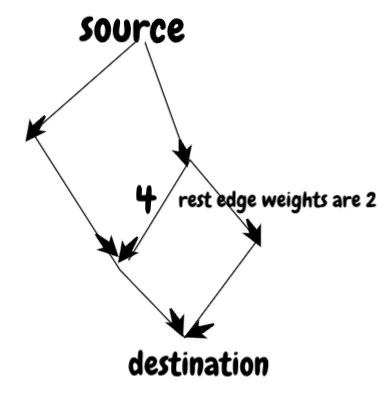
\includegraphics[width=0.5\textwidth,height=0.5\textheight,keepaspectratio]{bflow} 
    \item VIMP Note: if you are traversing through all 'v' like in the code above then its fine but otherwise if you do glist[u].pb(v) you \textbf{must} also do glist[v].pb (u) but only set res[u][v].
    \item Lets define an s-t cut C = (s-component, t-component) as a partition of V s.t. source s belongs to s-component and sink t belongs to t-component. Lets also define a cut-set to be set $\{(u, v) \in E | u \in s-comp, v \in t-comp\}$ such that if all edges in cut-set of C are removed, max flow from s to t is 0. (i.e. s and t are disconnected). The cost of an s-t cut C is defined by the sum of capacities of edges in cut-set of C. The min cut problem (min cut) is to minimize the amount of capacity of an s-t cut. Sol: After running max flow algo, do bfs/dfs from s, all vertices reachable from s using positive weighted edges in the residual graph belong to s-comp. and remaining belong to t-comp. and mf = min cut value. This is max-flow min-cut theorem.
    \item Multisource/multisink: Create a supersource ss and super sing st. Connect ss with all s with infinite capacity and also connect all t with st with infinte capacity, then run edmonds karps as per normal.
    \item Vertex capacities: Network flow variant where capacities are not just defined along the edges but also on the vertices. Split each v to vin and vout, reassigning its incomint/outgoing edges to vin/vout resp. and finally putting the original vertex v's weight as the weight of edge vin -$>$ vout. Note that this will double the number of vertices
    \item Max Independent paths: two paths are said to be independent if they do not share any vertex apart from s and t. Soln: construct a flow network N = (V, E) from G with vertex capacitites, where N is the carbon copy of G except that the capacity of each v in V is 1 (i.e. each vertex can only be used once) and the capacity of each edge e in V is also 1. Then run edmonds karps algo as per normal.
    \item Max edge disjoint paths: finding the maximum number of edge disjoint paths rom s to t is simlar to finding max independent paths. The only difference is that this time we do not have any vertex capacity (i.e. 2 edge disjoint paths can still share the same vertex)
    \item \href{https://uva.onlinejudge.org/external/5/563.pdf}{Crimewave}, \href{https://gist.github.com/sourabh2311/d9125c7f5149f80b267514b66ec65d3b}{sol} 
    \item \textbf{MWIS on a bipartite graph}
    \\Problem is equivalent to finding the minimum weight vertex cover in the graph. The latter can be solved using maximum flow techniques:
    \\Introduce a super-source S and a super-sink T. connect the nodes on the left side of the bipartite graph to S, via edges that have their weight as capacity. Do the same thing for the right side and sink T. Assign infinite capacity to the edges of the original graph.

    Now find the minimum S-T cut in the constructed network. The value of the cut is the weight of the minimum vertex cover. To see why this is true, think about the cut edges: They can't be the original edges, because those have infinite capacity. If a left-side edge is cut, this corresponds to taking the corresponding left-side node into the vertex cover. If we do not cut a left-side edge, we need to cut all the right-side edges from adjacent vertices on the right side.

    Thus, to actually reconstruct the vertex cover, just collect all the vertices that are adjacent to cut edges, or alternatively, the left-side nodes not reachable from S and the right-side nodes reachable from S.
    

\end{itemize}
\subsection{Minimum Cost Flow}
Given a network $G$ consisting of $n$ vertices and $m$ edges. For each edge (generally speaking, oriented edges, but see below), the capacity (a non-negative integer) and the cost per unit of flow along this edge (some integer) are given. Also the source $s$ and the sink $t$ are marked.

For a given value $K$, we have to find a flow of this quantity, and among all flows of this quantity we have to choose the flow with the lowest cost. This task is called minimum-cost flow problem.

Sometimes the task is given a little differently: you want to find the maximum flow, and among all maximal flows we want to find the one with the least cost. This is called the minimum-cost maximum-flow problem.

Both these problems can be solved effectively with the algorithm of sucessive shortest paths.

First we only consider the simplest case, where the graph is oriented, and there is at most one edge between any pair of vertices (e.g. if $(i, j)$ is an edge in the graph, then $(j, i)$ cannot be part in it as well).

Let $U_{i j}$ be the capacity of an edge $(i, j)$ if this edge exists. And let $C_{i j}$ be the cost per unit of flow along this edge $(i, j)$. And finally let $F_{i, j}$ be the flow along the edge $(i, j)$. Initially all flow values are zero.

We modify the network as follows: for each edge $(i, j)$ we add the reverse edge $(j, i)$ to the network with the capacity $U_{j i} = 0$ and the cost $C_{j i} = -C_{i j}$. Since, according to our restrictions, the edge $(j, i)$ was not in the network before, we still have a network that is not a multigraph (graph with multiple edges). In addition we will always keep the condition $F_{j i} = -F_{i j}$ true during the steps of the algorithm.

We define the residual network for some fixed flow $F$ as follow (just like in the Ford-Fulkerson algorithm): the residual network contains only unsaturated edges (i.e. edges in which $F_{i j} < U_{i j}$), and the residual capacity of each such edge is $R_{i j} = U_{i j} - F_{i j}$.

Now we can talk about the algorithms to compute the minimum-cost flow. At each iteration of the algorithm we find the shortest path in the residual graph from $s$ to $t$. In contrary to Edmonds-Karp we look for the shortest path in terms of the cost of the path, instead of the number of edges. If there doesn't exists a path anymore, then the algorithm terminates, and the stream $F$ is the desired one. If a path was found, we increase the flow along it as much as possible (i.e. we find the minimal residual capacity $R$ of the path, and increase the flow by it, and reduce the back edges by the same amount). If at some point the flow reaches the value $K$, then we stop the algorithm (note that in the last iteration of the algorithm it is necessary to increase the flow by only such an amount so that the final flow value doesn't surpass $K$).

It is not difficult to see, that if we set $K$ to infinity, then the algorithm will find the minimum-cost maximum-flow. So both variations of the problem can be solved by the same algorithm.

The case of an undirected graph or a multigraph doesn't differ conceptually from the algorithm above. The algorithm will also work on these graphs. However it becomes a little more difficult to implement it.

An undirected edge $(i, j)$ is actually the same as two oriented edges $(i, j)$ and $(j, i)$ with the same capacity and values. Since the above-described minimum-cost flow algorithm generates a back edge for each directed edge, so it splits the undirected edge into $4$ directed edges, and we actually get a multigraph.

How do we deal with multiple edges? First the flow for each of the multiple edges must be kept separately. Secondly, when searching for the shortest path, it is necessary to take into account that it is important which of the multiple edges is used in the path. Thus instead of the usual ancestor array we additionally must store the edge number from which we came from along with the ancestor. Thirdly, as the flow increases along a certain edge, it is necessary to reduce the flow along the back edge. Since we have multiple edges, we have to store the edge number for the reversed edge for each edge.

There are no other obstructions with undirected graphs or multigraphs.
\\Sample Prob: \href{https://uva.onlinejudge.org/external/105/10594.pdf}{UVA 10594}, \href{https://github.com/sourabh2311/Competitive-Programming/blob/master/UVA_10594_Better.cpp}{sol}
\subsection{Kirchhoff's matrix tree theorem}
Problem: You are given a connected undirected graph (with possible multiple edges) represented using an adjacency matrix. Find the number of different spanning trees of this graph.
\\Let $A$ be the adjacency matrix of the graph: $A_{u,v}$ is the number of edges between $u$ and $v$. Let $D$ be the degree matrix of the graph: a diagonal matrix with $D_{u,u}$ being the degree of vertex $u$ (including multiple edges and loops - edges which connect vertex $u$ with itself).
The Laplacian matrix of the graph is defined as $L = D - A$. According to Kirchhoff's theorem, all cofactors of this matrix are equal to each other, and they are equal to the number of spanning trees of the graph. The $(i,j)$ cofactor of a matrix is the product of $(-1)^{i + j}$ with the determinant of the matrix that you get after removing the $i$-th row and $j$-th column.\\ Thus we can get answer in $O(n^3)$.
\subsection{Counting Labeled graphs}
\subsubsection{Labeled graphs}

Let the number of vertices in a graph be $n$. We have to compute the number $G_n$ of labeled graphs with $n$ vertices (labeled means that the vertices are marked with the numbers from $1$ to $n$). The edges of the graphs are considered undirected, and loops and multiple edges are forbidden.

We consider the set of all possible edges of the graph. For each edge $(i, j)$ we can assume that $i < j$ (because the graph is undirected, and there are no loops). Therefore the set of all edges has the cardinality $\binom{n}{2}$, i.e. $\frac{n(n-1)}{2}$.

Since any labeled graph is uniquely determined by its edges, the number of labeled graphs with $n$ vertices is equal to: $$G_n = 2^{\frac{n(n-1)}{2}}$$
\subsubsection{Connected labeled graphs}

Here, we additionally impose the restriction that the graph has to be connected.

Let's denote the required number of connected graphs with $n$ vertices as $C_n$.

We will first discuss how many disconnected graphs exists. Then the number of connected graphs will be $G_n$ minus the number of disconnected graphs. Even more, we will count the number of disconnected, rooted graphs.A rooted graph is a graph, where we emphasize one vertex by labeling it as root. Obviously we have $n$ possibilities to root a graph with $n$ labeled vertices, therefore we will need to divide the number of disconnected rooted graphs by $n$ at the end to get the number of disconnected graphs.

The root vertex will appear in a connected component of size $1, \dots n-1$. There are $k \binom{n}{k} C_k G_{n-k}$ graphs such that the root vertex is in a connected component with $k$ vertices (there are $\binom{n}{k}$ ways to choose $k$ vertices for the component, these are connected in one of $C_k$ ways, the root vertex can be any of the $k$ vertices, and the remainder $n-k$ vertices can be connected/disconnected in any way, which gives a factor of $G_{n-k}$). Therefore the number of disconnected graphs with $n$ vertices is: $$\frac{1}{n} \sum_{k=1}^{n-1} k \binom{n}{k} C_k G_{n-k}$$ And finally the number of connected graphs is: $$C_n = G_n - \frac{1}{n} \sum_{k=1}^{n-1} k \binom{n}{k} C_k G_{n-k}$$
\subsubsection{Labeled graphs with $k$ connected components}

Based on the formula from the previous section, we will learn how to count the number of labeled graphs with $n$ vertices and $k$ connected components.

This number can be computed using dynamic programming. We will compute $D[i][j]$ - the number of labeled graphs with $i$ vertices and $j$ components - for each $i \le n$ and $j \le k$.

Let's discuss how to compute the next element $D[n][k]$ if we already know the previous values. We use a common approach, we take the last vertex (index $n$). This vertex belongs to some component. If the size of this component be $s$, then there are $\binom{n-1}{s-1}$ ways to choose such a set of vertices, and $C_s$ ways to connect them.After removing this component from the graph we have $n-s$ remaining vertices with $k-1$ connected components. Therefore we obtain the following recurrence relation: $$D[n][k] = \sum_{s=1}^{n} \binom{n-1}{s-1} C_s D[n-s][k-1]$$
\subsection{Heavy Light Decomposition}
We will divide the tree into vertex-disjoint chains ( Meaning no two chains has a node in common ) in such a way that to move from any node in the tree to the root node, we will have to change at most log N chains. Now the path from any node A to any node B can be  broken into two paths: A to LCA( A, B ) and B to LCA( A, B ).
\\We already know that queries in each chain can be answered with O( log N ) complexity and there are at most log N chains we need to consider per path. So on the whole we have $O(log^2 N)$ complexity solution.
\\Special Child : Among all child nodes of a node, the one with maximum sub-tree size is considered as Special child. Each non leaf node has exactly one Special child.
\\Special Edge : For each non-leaf node, the edge connecting the node with its Special child is considered as Special Edge.
\\What happens if you go to each node, find the special child and special edge and mark all special edges with green color and other edges are still black? Well, what happens is HLD. What would the graph look like then? Colorful yes. Not just colorful. Green edges actually forms vertex disjoint chains and black edges will be the connectors between chains. Let us explore one chain, start at root, move to the special child of root (there is only one special child, so easy pick), then to its special child and so on until you reach a leaf node, what you just traveled is a chain which starts at root node. Let us assume that root node has m child nodes. Note that all m-1 normal child nodes are starting nodes of some other chains.
\\When you move from a node to any of its normal child, the sub-tree size is at most half the sub-tree size of current node.
\\Changing a chain means we are moving for a node to a normal child, so each time we change chain we are at least halving the sub-tree size. For a tree with size N, we can halve it at most log N times.
\\\href{http://acm.timus.ru/problem.aspx?space=1&num=1553}{Timus 1553}, \href{https://github.com/sourabh2311/Competitive-Programming/blob/master/timus/1553.cpp}{Sol}
\subsection{More Problems}
\begin{itemize}
    \item \href{}{UVA 928}: just bfs with dp
    \item \href{https://uva.onlinejudge.org/external/102/10246.pdf}{That worst feast problem UVA 10246}, \href{https://gist.github.com/sourabh2311/e55a0e3f7453e4514f1251b1ae6f0827}{sol}
    \item \href{https://gist.github.com/sourabh2311/a9f9b7584631b8859692df0f4af0843d}{Atcoder}
    \item \href{https://codeforces.com/problemset/problem/986/C}{986C AND graph}, \href{https://codeforces.com/blog/entry/59758}{Sol}
\end{itemize}
\section{Some Basic}
\begin{itemize}
    \item 
\begin{minted}{cpp}
#pragma GCC optimize("Ofast")  // tells the compiler to optimize the code for speed to make it as fast as possible (and not look for space)
#pragma GCC optimize ("unroll-loops")  // normally if we have a loop there is a "++i" instruction somewhere. We normally dont care because code inside the loop requires much more time but in this case there is only one instruction inside the loop so we want the compiler to optimize this.
#pragma GCC target("sse,sse2,sse3,ssse3,sse4,popcnt,abm,mmx,avx,tune=native")  // tell the compiler that our cpu has simd instructions and allow him to vectorize our code
\end{minted}
\begin{minted}{cpp}
// Backtracking
void bktk () {
    if (state == complete ) {
        // process it
    } else {
        for each possible next move P {
            apply move P;
            bktk ();
            undo move P;
        }
    }
}
// ex1: generating permutations O(n! * n)
// better use next_permutation. 
// think of doing such things for n <= 11. 11! ~ 4 * 10^7
void bktk () {
    if (perm.size () == n) {
        // process permutation 
    } else {
        for (int i = 0; i < n; i++) {
            if (!chosen[i]) {
                chosen[i] = true;
                perm.push_back (i);
                bktk ();
                perm.pop_back ();
                chosen[i] = false;
            }
        }
    }
}
// ex2: generating subsets
void bktk (int k) {
    if (k == n) {
        // process subset
    } else {
        // Move one is to not push it and move 2 is to consider it.
        bktk (k + 1);
        subset.push_back(k);
        bktk (k + 1);
        subset.pop_back;
    }
}
// better way to generate subsets O(2^n) so valid for n <= 25. So whenever you see this, think of iterating through subsets
// 1 << 0 = 1.
for (int i = 0; i < (1 << n); i++) {
    for (int b = 0; b < n; b++) {
        if (i & (1 << b)) {
            subset.pb (b);
        }
        // process subset
    }
}
\end{minted}
    \item $\leq 10^8 \Rightarrow 2$ sec.
    \item Remember that just like we could have solved \href{https://uva.onlinejudge.org/external/7/714.pdf}{this} using binary search (other than simple DP), we can actually solve many problems which ask to find optimal value using binary search.
    \item Outputing a double or even int my have an exponential form so it is better to do << fixed << s...(0).
    \item Range of double is $10^{15}$
    \item Range of int64 is $9 * 10^{18}$
    \item Inbuilt swap can be used to basically swap anything.
    \item $ceil(m/a) = (m + a - 1) / m$
    \item Consider $m*n$ surface, you have a sq. of size $a*a$. Min. no. of squares to cover completely the surface? Ans: $ceil(m/a)*ceil(n/a)$
    \item Not neccessary to cover the border cells? Ans: $m/a * n/a$
    \item Note: Sides of the square must be parallel to grid.
    \item  lower\_bound Returns an iterator pointing to the first element in the range [first,last) which does not compare less than val. Unlike upper\_bound, the value pointed by the iterator returned by this function may also be equivalent to val, and not only greater. If all the element in the range compare less than val, the function returns last.
    \item upper\_bound Returns an iterator pointing to the first element in the range [first,last) which compares greater than val. If no element in the range compares greater than val, the function returns last.
    \item 
    \begin{minted}{cpp}
    /* we need to do binary search for range [st + 1, en - 1], i.e. [st + 1, en). */
        if (binary_search (arr.begin() + st + 1, arr.begin() + en, leftover_))
    \end{minted}
    \item If you want to iterate through subsets of fixed size k, you may want to use k for loops.
    \item or a better way is, considering a set of numbers from 1 to n,The first combination will be 1, 2, ..., k. Now let's see how to find the combination that immediately follows this, lexicographically. To do so, we consider our current combination, and find the rightmost element that has not yet reached its highest possible value. Once finding this element, we increment it by 1, and assign the lowest valid value to all subsequent elements.
\begin{minted}{cpp}
bool next_combination(vector<int>& a, int n) {
    int k = (int)a.size();
    for (int i = k - 1; i >= 0; i--) {
        if (a[i] < n - k + i + 1) {
            a[i]++;
            for (int j = i + 1; j < k; j++)
                a[j] = a[j - 1] + 1;
            return true;
        }
    }
    return false;
}
\end{minted}
    \item \href{https://uva.onlinejudge.org/external/4/410.pdf}{UVA 410 Load Balancing}, \href{https://gist.github.com/sourabh2311/5405601b47b1bd9c8fa769c82b280328}{sol}
    \item \href{https://uva.onlinejudge.org/external/104/10440.pdf}{ferry loading}, \href{https://gist.github.com/sourabh2311/4af5bc294ab613057de828b308da587a}{sol}, just know that best time is last cars arrival + t/2, so just achieve it.
    \begin{minted}{cpp}
    One can write i = (m % n == 0 ? n - 1 : m % n - 1) as
    i = (m + n - 1) % n.
    \end{minted}
    \begin{minted}{cpp}
    We can use cin.peek () to see the next available character
    \end{minted}
    \item
    \begin{minted}{cpp}
    1011101010000000 >>= 8 => num is 10111010 similarly num <<= 8 implies num is 10000000
    \end{minted}
    \item tictactoe game starts by placing 'X' so if in between $O_cnt = X_cnt$ and X has win that means invalid game. And if $O_cnt + 1 = X_cnt$ and O has win that means not a valid game.
    \item 
    \begin{eqnarray}
    24_{hours} & = & 10_{decimalHours} \\
    24 * 60 * 60 * 100_{normalCC} & = & 10 * (100^3)_{decimalCC} \\
    1_{decimalCC} & = & 0.864_{normalCC} 
    \end{eqnarray}
    that means $1_{nCC} * (1_{dCC}/0.864_{nCC})$ Would give us dCC
    \item XOR is associative and commutative
    \item x\^{}x = 0, x\^{}0 = x.
    \item x\^{}(string of 1's, i.e. (\~{}0)) = \~{}x
    \item x\^{}y = x\^{}z implies y = z. (how? just take xor with x on both sides)
    \item Swapping 2 nos with XOR
    \begin{minted}{cpp}
x = A, y = B;
x = x ^ y;
y = x ^ y; // i.e. (A ^ B) ^ B = A
x = x ^ y; // i.e. (A ^ B) ^ A = B
    \end{minted}
    \item \href{}{UVA 10309 Lights off}:
    \begin{minted}{cpp}
    This problem is solved using complete search technique. Notice that each bulb can be toggled by 3 switches on the same row and 1 switch on the upper row and another one on the lower row, keep this in mind as we will use it later. Our solution has three steps: 1. For the first row try all 2^10 possible combinations of switches. We expect to have some switches turned on after this step. 2. For the rest of the rows, toggle switch (i, j) if (i-1, j) is switched on, this means toggle any switch if the bulb above it (in the previous row is turned on). This step insures that all bulbs will be turned off using the switch in the next row, except the last row, as there is no next row. 3. Check the bulbs in the last row, if all bulbs are turned off, then the current solution if valid, if any of the bulbs is on, this solution is not valid. Keep track of the number of switches toggled in each solution, and the final result is their minimum value.
    \end{minted}
    \item \begin{minted}{cpp}
while (first || cin >> temp) {  // something }
            \end{minted}
    \item \textbf{Interval Covering: }Tell the minimum no. of intervals to cover the entire big interval.
    \begin{minted}{cpp}
void solve() {
    // Greedy Algorithm
    sort (data.begin (), data.end ()); 
    for (; i < data.size(); i = j) {
       if (data[i].first > rightmost) break;
       for (j = i + 1; j < data.size() and data[j].first <= rightmost; j++) {
           if (data[j].second > data[i].second) {
               i = j;
           }
       }
       ans.push_back(data[i]);
       rightmost = data[i].second;
       if (rightmost >= m) break;

    }
    if (rightmost < m) {
       cout << "0\n";
    }
}

    \end{minted}
    \item \textbf{Prob: }We have a stack of turtles and we have some final permutation of them, each turtule can crawl out of its position and move to top. Determine a minimal sequence of operations to obtain the final permutation.\\\textbf{Sol: }
    \begin{minted}{cpp}
for (int j = n - 1, next = n - 1; j >= 0; j--) {
    if (order[j].second != next) Toswap.push_back(order[j]);
    else next--;
}
sort (Toswap.begin(), Toswap.end());
\end{minted}
    \item \begin{minted}{cpp}
        #define MAX_N 2 // Fibonacci matrix, increase/decrease this value as needed
struct Matrix { int mat[MAX_N][MAX_N]; }; // we will return a 2D array
Matrix matMul(Matrix a, Matrix b) { // O(n^3)
   Matrix ans; int i, j, k;
   for (i = 0; i < MAX_N; i++)
       for (j = 0; j < MAX_N; j++)
           for (ans.mat[i][j] = k = 0; k < MAX_N; k++) // if necessary, use
               ans.mat[i][j] += a.mat[i][k] * b.mat[k][j]; // modulo arithmetic
   return ans;
}
Matrix matPow(Matrix base, int p) { // O(n^3 log p)
   Matrix ans; int i, j;
   for (i = 0; i < MAX_N; i++) for (j = 0; j < MAX_N; j++)
           ans.mat[i][j] = (i == j); // prepare identity matrix
   while (p) { // iterative version of Divide & Conquer exponentiation
       if (p & 1) ans = matMul(ans, base); // if p is odd (last bit is on)
       base = matMul(base, base); // square the base
       p >>= 1; // divide p by 2
   }
   return ans;
}
    \end{minted}
    \item \begin{minted}{cpp}
// Months are 0 indexed
//The following Code solves problems: UVA 893 

int numberDaysInMonth[] = {31, 28, 31, 30, 31, 30, 31, 31, 30, 31, 30, 31};
int numberDaysInMonthLeap[] = {31, 29, 31, 30, 31, 30, 31, 31, 30, 31, 30, 31};

bool IsLeapYear(int year)
{
   return year % 4 == 0 && (year % 100 != 0 || year % 400 == 0);
}

int MonthToDay(int month, int year)
{
   int daysBefore = 0;
   for (int i = 0; i < month; ++i)
       daysBefore += numberDaysInMonth[i];
   if (month > 1 && IsLeapYear(year))
       ++daysBefore;
   return daysBefore;
}

int YearToDay(int year)
{
   int base = year * 365;
   int numLeapYears = year / 4 - year / 100 + year / 400;
   return base + numLeapYears;
}

int GetYearFromNumDays(int& numDays)
{
   int year = 1;
   int sizeOfYear = 365;

   while (numDays > sizeOfYear)
   {
       numDays -= sizeOfYear;
       ++year;
       sizeOfYear = (IsLeapYear(year)) ? 366 : 365;
   }

   return year;
}

int GetMonthFromNumDays(int& numDays, int year)
{
   int month = 0;
   int * numDayUsed = (IsLeapYear(year)) ? numberDaysInMonthLeap : numberDaysInMonth;
   for (;numDays > numDayUsed[month]; ++month)
       numDays -= numDayUsed[month];
   return month + 1;
}

int main()
{
   int dayForward, day, month, year;
   while (cin >> dayForward >> day >> month >> year, year)
   {
       --month;
       day += MonthToDay(month, year);
       --year;
       day += YearToDay(year);
       day += dayForward;

       year = GetYearFromNumDays(day);
       month = GetMonthFromNumDays(day, year);
       cout << day << ' ' << month << ' ' << year << '\n';
   }
}
//--
string int2roman(int n) {
   string roman;
   string ones[] = {"", "I", "II", "III", "IV", "V", "VI", "VII", "VIII", "IX"};
   string tens[] = {"", "X", "XX", "XXX", "XL", "L", "LX", "LXX", "LXXX", "XC"};
   string hundreds[] = {"", "C", "CC", "CCC", "CD", "D", "DC", "DCC", "DCCC", "CM"};
   string thousands[] = {"", "M", "MM", "MMM"};

   int o = n % 10;
   n /= 10;
   int t = n % 10;
   n /= 10;
   int h = n % 10;
   n /= 10;
   int th = n % 10;

   roman += thousands[th] + hundreds[h] + tens[t] + ones[o];//Or
   //roman=thousands[th] + hundreds[h] + tens[t] + ones[o] but the written one is
   //faster.

   return roman;
}

    \end{minted}
    \item \textbf{Algorithm to convert from infix to postifx: }
        \begin{enumerate}
        \item Scan the infix expression from left to right.
        \item If the scanned character is an operand, output it.
        \item Else,
            \begin{enumerate}
            \item If the precedence of the scanned operator is greater than the precedence of the operator in the stack (or the stack is empty or the stack contains a ‘(‘ ), push it.
            \item  Else, Pop all the operators from the stack which are greater than or equal to in precedence than that of the scanned operator. After doing that Push the scanned operator to the stack. (If you encounter parenthesis while popping then stop there and push the scanned operator in the stack.)
            \end{enumerate}
        \item If the scanned character is an ‘(‘, push it to the stack.
        \item If the scanned character is an ‘)’, pop the stack and and output it until a ‘(‘ is encountered, and discard both the parenthesis.
        \item Repeat steps 2-6 until infix expression is scanned.
        \item Print the output
        \item Pop and output from the stack until it is not empty.
        \end{enumerate}
    \item \textbf{Algorithm to convert from infix to prefix: }
        \begin{enumerate}
        \item Properly reverse the infix exp.
        \item Gets its postfix as above
        \item Reverse postfix and output it.
        \end{enumerate}
    \item \textbf{Algorithm to convert from postfix to infix: }
        \begin{enumerate}
        \item If the symbol is an operand, push it onto stack
        \item Else, if there are fewer than two values in stack, show error. Else, pop top 2 expressions from stack (say e1, e2), put the operator (op) between them and push to stack ((e1 op e2))
        \item After reading postfix expression, Stack should have only one item which is our answer 
        \end{enumerate}
    \item \textbf{Merge Sort}
    \begin{minted}{cpp}
    // IMP NOTE: In both bubble sort and merge sort we are getting minimum no. of swaps to sort an array (i.e. by swapping adjacent elements)
void merge(int arr[], int l, int m, int r)
{
   int i, j, k;
   int n1 = m - l + 1;
   int n2 =  r - m;

   /* create temp arrays */
   int L[n1], R[n2];

   /* Copy data to temp arrays L[] and R[] */
   for (i = 0; i < n1; i++)
       L[i] = arr[l + i];
   for (j = 0; j < n2; j++)
       R[j] = arr[m + 1+ j];

   /* Merge the temp arrays back into arr[l..r]*/
   i = 0; // Initial index of first subarray
   j = 0; // Initial index of second subarray
   k = l; // Initial index of merged subarray
   while (i < n1 && j < n2)
   {
       if (L[i] <= R[j])
       {
           arr[k] = L[i];
           i++;
       }
       else///i.e we need to swap
       {
           arr[k] = R[j];
           swaps+=n1-i;//Most important line. basically once we are doing arr[k]=R[j] that means we are
           ///putting R[j] before each of n1-i elements thus there are that many swaps.
           j++;
       }
       k++;
   }

   /* Copy the remaining elements of L[], if there
      are any */
   while (i < n1)
   {
       arr[k] = L[i];
       i++;
       k++;
   }

   /* Copy the remaining elements of R[], if there
      are any */
   while (j < n2)
   {
       arr[k] = R[j];
       j++;
       k++;
   }
}

/* l is for left index and r is right index of the
  sub-array of arr to be sorted */
void mergeSort(int arr[], int l, int r)
{
   if (l < r)
   {
       // Same as (l+r)/2, but avoids overflow for
       // large l and h
       int m = l+(r-l)/2;

       // Sort first and second halves
       mergeSort(arr, l, m);
       mergeSort(arr, m+1, r);

       merge(arr, l, m, r);
   }
}
    \end{minted}
    \item set is like min heap. Only unique elements are present.
    \item On a line you are given the x coordinates of various houses, tell the house of vito (h) such that $\sum |h_i - h|$ is minimised. \textbf{Obs1: } h could be any of $h_i$ so $O(n^2)$ algo. will work. \textbf{Obs2: } Taking derivative we get $i - j = 0$ i.e. $i = j = n/2$, that means simply sort and output the middlemost house.\\
    \textbf{Note: }Some times the math become cumbersome, in such cases, use \textbf{ternary search}
    \item \textbf{Prob: }n people have to cross the bridge, one torch, atmost 2 can travel\\
    \textbf{Sol: }if $n = 3 \Rightarrow$ time = $x + y + z$, if $n \geq 4$ let A, B, a, b be the fastest, second fastest, slowest, second slowest resp. \textbf{Goal: }Get the slowest members to the other side. So choose the best among the two options.\\\textbf{option 1: }Fastest member does back and forth.\\\textbf{option 2: }The two fastest members go, allowing the two slowest two to go together.
    \item \textbf{Inversions: }From a permutation, parity of number of swaps needed to get to the identical permutation is same as parity of inversion count of this permutation.
    \\Parity of inversions can be calculated in $O(n)$ by finding the number of cycles. Consider the permutation [5, 2, 4, 3, 6, 1], if we view the permutation as a mapping from [1, 2, 3, 4, 5, 6] to [5, 2, 4, 3, 6, 1] the permutation can be decomposed into disjoint cycles. A cycle is a subset of elements that map to each other. For example, 1 gets mapped to 5, which gets mapped to 6, which gets mapped back to 1. So one cycle is [1, 5, 6]. The other cycles are [2] and [3, 4]. Thus the no. of cycles for this permutation is 3. Parity of $n -$ no. of cycles = parity of inversions.
    \begin{minted}{cpp}
    for (int i = 1; i <= n; i++) {  // 1 indexed
        if (was[i]) continue;
        cyc++;
        int p = i;
        while (!was[p]) {
            was[p] = 1;
            p = a[p];
        }
    }
    \end{minted}
    \item Exact value of number of inverions can be calculated in $(nlog(n))$ by using segment trees. 
    \item \textbf{Prob: }You are given two positive integer numbers a and b. Permute (change order) of the digits of a to construct maximal number not exceeding b.
    \\\textbf{Sol: }Take the number as string. sort string a, then for each $i \in [1, n]$ swap it with $j$ trying from $n to i + 1$ such that it is $\leq b$ (normal string comparison can be used).
    \item \textbf{Prob: }From a digraph, remove atmost one edge so that it becomes DAG.
    \\\textbf{Sol: }Get any one cycle the iteratively try to remove each edge and see if it makes it DAG or not.
    \item \textbf{UFDS}
    \begin{minted}{cpp}
struct UFDS {
    vector<int> p, rank, setSizes;
    int numSets;
    UFDS(int N) {
        numSets = N;
        rank.assign(N, 0);
        p.assign(N, 0);
        for (int i = 0; i < N; i++)
            p[i] = i;
        setSizes.assign(N, 1);
    }
    int findSet(int i) {
        return (p[i] == i) ? i : p[i] = findSet(p[i]);
    }
    bool isSameSet(int i, int j) {
        return findSet(i) == findSet(j);
    }
    void unionSet(int i, int j) {
        if (!isSameSet(i, j)) {
            int x = findSet(i), y = findSet(j);
            if (rank[x] > rank[y]) {
                setSizes[findSet(x)] += setSizes[findSet(y)];
                p[y] = x;
            } else {
                setSizes[findSet(y)] += setSizes[findSet(x)];
                p[x] = y;
                if (rank[x] == rank[y])
                    rank[y]++;
            }
            numSets--;
        }
    }
    int setSize(int i) {
        return setSizes[findSet(i)];
    }
    int numDisjointSets() {
        return numSets;
    }
};
    \end{minted}
    \item \href {https://uva.onlinejudge.org/external/101/10158.pdf}{UVA 10158 Prob}, \href {https://gist.github.com/sourabh2311/3a2daf2a9f77104a94d1db9af8b40b1a}{UVA 10158 Sol}
    \item \href {https://codeforces.com/contest/915/problem/F}{Imbalance of a tree}, \href {https://github.com/sourabh2311/Competitive-Programming/blob/master/CF/ER36/F.cpp}{Sol}, summation(max - min) is same as summation(max) - summation(min).
    \item \href {https://codeforces.com/contest/913/problem/C}{Party Lemonade}, \href {https://codeforces.com/contest/913/submission/34067096}{Sol}
    \item \href {https://codeforces.com/contest/916/problem/B}{Jamie and binary sequence}, \href {https://github.com/sourabh2311/Competitive-Programming/blob/master/CF/457D2/B.cpp}{Sol}.
    \item \href {https://codeforces.com/contest/912/problem/E}{Prime gift}, \href {https://codeforces.com/contest/912/submission/33976448}{Sol}. awesome 2 pointers problem.
    \item \href {https://codeforces.com/contest/912/problem/D}{Fishes}, \href {https://codeforces.com/blog/entry/56920}{Sol}. 
    \item \textbf{Max 1D Range Sum (kadane)}
    \begin{minted}{cpp}
sum = ans = 0;
finish = -1;
local_start = 0;
for (int i = 0; i < n ;i++) {
    sum += A[i];
    if (sum > ans) {
        ans = sum;
        start = local_start;
        finish = i;
    }
    if (sum < 0) {
        sum = 0;
        local_start = i + 1;
    }
}
// if instead of maximum you want to find minimum, simply negate all terms. As suppose minimum sum is (ak, a_{k + 1}, ..., a_{k + l}) which must be negative and most (maximum in other dirn) negative possible. Thus (-ak,...) is maximum positive possible as suppose there was some other range with maximum possible that means its negative (actual) is more minimum then our current which leads to contradiction
    \end{minted}
    \item \textbf{Max 2D range sum, algo1}
    \begin{minted}{cpp}
// grid need not be square
// O(n^4)
// Commented part shows for torus
cin >> n;
for (int i = 0; i < n; i++) { // < 2n
    for (int j = 0; j < n; j++) { // <2n
        cin >> A[i][j]; 
        /*
        if (i < n and j < n) {
            cin >> A[i][j];
            A[i + n][j] = A[i][j + n] = A[i + n][j + n] = A[i][j];
        }
        */
        if (i) A[i][j] += A[i - 1][j];
        if (j) A[i][j] += A[i][j - 1];
        if (i and j) A[i][j] -= A[i - 1][j - 1];
    }
    int maxSubRect = -127 * 100 * 100;
    for (int i = 0; i < n; i++) {
        for (int j = 0; j < n; j++) {
            for (int k = i; k < n; k++) {  // < i + n
                for (int l = j; l < n; l++) {  // < j + n
                    subRect = A[k][l];
                    if (i) subRect -= A[i - 1][l];
                    if (j) subRect -= A[k][j - 1];
                    if (i and j) subRect += A[i - 1][j - 1];
                    maxSubRect = max (maxSubRect, subRect);
                }
            }
        }
    }
// "No tree" => make tree (1) = -inf
// no tree (0) = 1.
}
    \end{minted}
    \item \textbf{Max 2D range sum, algo1} 
    \begin{minted}{cpp}
// O(n^3)
int maxSum2D () {
    int maxsum = INT_MIN, finalleft, finalright, finaltop, finalbottom;
    for (int leftc = 0; leftc < COL; leftc++) {
        vector<int> temp (ROW, 0);
        for (int rightc = leftc; rightc < COL; rightc++) {
            for (int i = 0; i < ROW; i++) {
                temp[i] += M[i][rightc]
            }
            int rstart, rend;
            sum = kadane (temp, rstart, rend);
            // kadane will give us rstart and rend
            if (sum > maxsum) {
                maxsum = sum;
                finalleft = left;
                finalright = right;
                finaltop = rstart;
                finalbottom = rend;
            } 
        }
    }
}
    \end{minted}
    \item Given an $n*m$ graph with each cell containing either 0 or 1, count how many rectangles can be formed by using the 1s (UVA 10502), Precalculate array sum[i][j],the numbers of 1 from graph[1][1] to graph[i][j] (index starting from 1 would be easier to deal with around edges) using $sum[i][j] = sum[i-1][j]+sum[i][j-1]-sum[i-1][j-1] + graph[i][j]-'0'$. Thus use algo1 of max 2d range.
    Then we could iterate through all possible rectangle in the given size in $O(n^4)$
    \item A problem is said to have optimal substructure if an optimal solution can be constructed from optimal solutions of its subproblems.
    \item A problem must exhibit these two properties in order for a greedy algorithm to work.
    \begin{itemize}
        \item It has optimal substructures
        \item It has the greedy property (if we make a choice that seems like the best at the moment and proceed to solve the remaining subproblem, we reach the optimal soln. We will never have to reconsider our previous choices)
    \end{itemize}
    \item \textbf{Stack Sorting: }If there exist a way to perform the operations such that array b is sorted in non descending order in the end then array a is called stack sortable. Operations availabe:
    \begin{enumerate}
        \item Take the first element of a, push it into S and remove it from a.
        \item Take the top element from S, append it to the end of array b and remove it from S.
    \end{enumerate}
    If you think about it you can see that problem occurs if we have sequence (x, y, z) where z < x < y. So after an element we want either all elements which are smaller than it to come first than elements which are bigger than it or all elements bigger than it. So say if we are given prefix of some permutation as [6, 3, 1] and asked to find lexicographic sequence to append such that it is stack sortable then we can read prefix number one by one and do\\
    $6 + A(1, 5) + A(7, 7)$\\
    $6 + 3 + A(1, 2) + A(4, 5) + A(7, 7)$\\
    $6 + 3 + 1 + 2 + 5 + 4 \text{ i.e. reverse each A(l, r) } + 7$\\
    And if at any time we couldn't proceed as desired that means soln does not exist.
    \item stoi, stol, stoll, stod
    \item to\_{}string
    \item 
    \begin{minted}{cpp}
int __builtin_clz(int x);// number of leading zero
int __builtin_ctz(int x);// number of trailing zero
int __builtin_clzll(long long x);// number of leading zero
int __builtin_ctzll(long long x);// number of trailing zero
int __builtin_popcount(int x);// number of 1-bits in x
int __builtin_popcountll(long long x);// number of 1-bits in x

lsb(n): (n & -n); // last bit (smallest)
floor(log2(n)): 31 - __builtin_clz(n | 1);
floor(log2(n)): 63 - __builtin_clzll(n | 1);
// Suppose we have a pattern of N bits set to 1 in an integer and we want the next permutation of N 1 bits in a lexicographical sense. For example, if N is 3 and the bit pattern is 00010011, the next patterns would be 00010101, 00010110, 00011001,00011010, 00011100, 00100011, and so forth. The following is a fast way to compute the next permutation.

unsigned int v; // current permutation of bits 
unsigned int w; // next permutation of bits

unsigned int t = v | (v - 1); // t gets v's least significant 0 bits set to 1
// Next set to 1 the most significant bit to change, 
// set to 0 the least significant ones, and add the necessary 1 bits.
w = (t + 1) | (((~t & -~t) - 1) >> (__builtin_ctz(v) + 1));  
    \end{minted}
\end{itemize}
\subsection{Meet in the middle}
Given a set of n integers where $n \leq 40$. Each of them is at most $10^{12}$, determine the maximum sum subset having sum less than or equal S where S <= $10^{13}$.

Example:

Input  : set[] = {45, 34, 4, 12, 5, 2} and S = 42
Output : 41
Maximum possible subset sum is 41 which can be obtained by summing 34, 5 and 2.

Input  : Set[] = {3, 34, 4, 12, 5, 2} and S = 10
Output : 10
Maximum possible subset sum is 10 which can be obtained by summing 2, 3 and 5.

A Brute Force approach to solve this problem would be find all possible subset sums of N integers and check if it is less than or equal S and keep track of such a subset with maximum sum. The time complexity using this approach would be $O(2^n)$ and n is at most 40. 240 will be quite large and hence we need to find more optimal approach.

Meet in the middle is a search technique which is used when the input is small but not as small that brute force can be used. Like divide and conquer it splits the problem into two, solves them individually and then merge them. But we can’t apply meet in the middle like divide and conquer because we don’t have the same structure as the original problem.

    Split the set of integers into 2 subsets say A and B. A having first n/2 integers and B having rest.
    Find all possible subset sums of integers in set A and store in an array X. Similarly calculate all possible subset sums of integers in set B and store in array Y. Hence, Size of each of the array X and Y will be at most $2^{n/2}$.
    Now merge these 2 subproblems. Find combinations from array X and Y such that their sum is less than or equal to S.
        One way to do that is simply iterate over all elements of array Y for each element of array X to check the existence of such a combination. This will take $O((2^{n/2})^2)$ which is equivalent to $O(2^n)$.
        To make it less complex, first sort array Y and then iterate over each element of X and for each element x in X use binary search to find maximum element y in Y such that $x + y \leq S$.
        Binary search here helps in reducing complexity from $2^n$ to $2^{n/2} \log{2^{n/2}}$ which is equivalent to $2^{n/2} *n$.

\begin{minted}{cpp}
// C++ program to demonstrate working of Meet in the 
// Middle algorithm for maximum subset sum problem. 
#include <bits/stdc++.h> 
using namespace std; 
typedef long long int ll; 
ll X[2000005],Y[2000005]; 
  
// Find all possible sum of elements of a[] and store 
// in x[] 
void calcsubarray(ll a[], ll x[], int n, int c) 
{ 
    for (int i=0; i<(1<<n); i++) 
    { 
        ll s = 0; 
        for (int j=0; j<n; j++) 
            if (i & (1<<j)) 
                s += a[j+c]; 
        x[i] = s; 
    } 
} 
  
// Returns the maximum possible sum less or equal to S 
ll solveSubsetSum(ll a[], int n, ll S) 
{ 
    // Compute all subset sums of first and second 
    // halves 
    calcsubarray(a, X, n/2, 0); 
    calcsubarray(a, Y, n-n/2, n/2); 
  
    int size_X = 1<<(n/2); 
    int size_Y = 1<<(n-n/2); 
  
    // Sort Y (we need to do doing binary search in it) 
    sort(Y, Y+size_Y); 
  
    // To keep track of the maximum sum of a subset 
    // such that the maximum sum is less than S 
    ll max = 0; 
  
    // Traverse all elements of X and do Binary Search 
    // for a pair in Y with maximum sum less than S. 
    for (int i=0; i<size_X; i++) 
    { 
        if (X[i] <= S) 
        { 
            // lower_bound() returns the first address 
            // which has value greater than or equal to 
            // S-X[i]. 
            int p = lower_bound(Y, Y+size_Y, S-X[i]) - Y; 
  
            // If S-X[i] was not in array Y then decrease 
            // p by 1 
            if (p == size_Y || Y[p] != (S-X[i])) 
                p--; 
  
            if ((Y[p]+X[i]) > max) 
                max = Y[p]+X[i]; 
        } 
    } 
    return max; 
} 
  
// Driver code 
int main() 
{ 
    ll a[] = {3, 34, 4, 12, 5, 2}; 
    int n=sizeof(a)/sizeof(a[0]); 
    ll S = 10; 
    printf("Largest value smaller than or equal to given "
           "sum is %lld\n", solveSubsetSum(a,n,S)); 
    return 0; 
} 

Output: Largest value smaller than or equal to given sum is 10
\end{minted}
\subsection{To find subarray (continguous) with maximum average and of length k}
It doesnt make sense to introduce average here as our length is fixed, so it just asks to find maximum sum subarray of length k. Which is easy to compute by simply using sliding window.
\begin{minted}{cpp}

// C++ program to find maximum average subarray 
// of given length. 
#include<bits/stdc++.h> 
using namespace std; 
  
// Returns beginning index of maximum average 
// subarray of length 'k' 
int findMaxAverage(int arr[], int n, int k) 
{ 
    // Check if 'k' is valid 
    if (k > n) 
        return -1; 
  
    // Compute sum of first 'k' elements 
    int sum = arr[0]; 
    for (int i=1; i<k; i++) 
        sum += arr[i]; 
  
    int max_sum = sum, max_end = k-1; 
  
    // Compute sum of remaining subarrays 
    for (int i=k; i<n; i++) 
    { 
        int sum = sum + arr[i] - arr[i-k]; 
        if (sum > max_sum) 
        { 
            max_sum = sum; 
            max_end = i; 
        } 
    } 
  
    // Return starting index 
    return max_end - k + 1; 
} 
  
// Driver program 
int main() 
{ 
    int arr[] = {1, 12, -5, -6, 50, 3}; 
    int k = 4; 
    int n = sizeof(arr)/sizeof(arr[0]); 
    cout << "The maximum average subarray of "
         "length "<< k << " begins at index "
         << findMaxAverage(arr, n, k); 
    return 0; 
} 
\end{minted}
\subsection{To find subarray (contiguous) with maximum average and length more than \textbf{k}}
Clearly we could have done this in $O(n^2)$ but i'll describe $O(n \log n)$ soln below.
\begin{enumerate}
    \item Binary search for the maximum average (let it be x)
    \item Subtract x from every element of array
\\Now the problem reduces to finding longest subarray with sum $\geq 0$ as then average would be $\geq 0$.
    \item Replace $a_i$ by the partial sums $S_i = \sum_{j = 1}^i a_j$\\
Now we are looking for a pair $0 \leq l \leq r \leq N$ s.t. $S_r - S_{l - 1} \geq 0$ and $r - (l - 1) \geq k$.
    \item Mark the positions of mimimas of $S_i$ from left to right in array A and position for maximums $S_i$ from right to left in array B of an array containing S.
    \item Do 2 pointers technique now.
\end{enumerate}
\begin{minted}{cpp}
// This is the code for steps 2-5.
int maxIndexDiff(int arr[], int n) 
{ 
    int maxDiff; 
    int i, j; 
  
    int LMin[n], RMax[n]; 
  
    // Construct LMin[] such that LMin[i] 
    // stores the minimum value 
    // from (arr[0], arr[1], ... arr[i]) 
    LMin[0] = arr[0]; 
    for (i = 1; i < n; ++i) 
        LMin[i] = min(arr[i], LMin[i - 1]); 
  
    // Construct RMax[] such that RMax[j] 
    // stores the maximum value 
    // from (arr[j], arr[j+1], ..arr[n-1]) 
    RMax[n - 1] = arr[n - 1]; 
    for (j = n - 2; j >= 0; --j) 
        RMax[j] = max(arr[j], RMax[j + 1]); 
  
    // Traverse both arrays from left to right 
    // to find optimum j - i 
    // This process is similar to merge() 
    // of MergeSort 
    i = 0, j = 0, maxDiff = -1; 
    while (j < n && i < n) { 
        if (LMin[i] < RMax[j]) { 
            maxDiff = max(maxDiff, j - i); 
            j = j + 1; 
        } 
        else
            i = i + 1; 
    } 
  
    return maxDiff + 1; 
} 
  
// utility Function which subtracts X from all 
// the elements in the array 
void modifyarr(int arr[], int n, int x) 
{ 
    for (int i = 0; i < n; i++) 
        arr[i] = arr[i] - x; 
} 
  
// Calculating the prefix sum array 
// of the modified array 
void calcprefix(int arr[], int n) 
{ 
    int s = 0; 
    for (int i = 0; i < n; i++) { 
        s += arr[i]; 
        arr[i] = s; 
    } 
} 
  
// Function to find the length of the longest 
// subarray with average >= x 
int longestsubarray(int arr[], int n, int x) 
{ 
    modifyarr(arr, n, x); 
    calcprefix(arr, n); 
  
    return maxIndexDiff(arr, n); 
} 
  
// Driver code 
int main() 
{ 
    int arr[] = { 1, 1, 2, -1, -1, 1 }; 
    int x = 1; 
    int n = sizeof(arr) / sizeof(int); 
    cout << longestsubarray(arr, n, x) << endl; 
  
    return 0; 
} 
\end{minted}
\subsection{Find subarray with given sum, elements are non negative}
\begin{minted}{cpp}

/* A simple program to print subarray with sum as given sum */
#include<stdio.h> 
  
/* Returns true if the there is a subarray of arr[] with sum equal to 'sum' 
   otherwise returns false.  Also, prints the result */
int subArraySum(int arr[], int n, int sum) 
{ 
    int curr_sum, i, j; 
  
    // Pick a starting point 
    for (i = 0; i < n; i++) 
    { 
        curr_sum = arr[i]; 
  
        // try all subarrays starting with 'i' 
        for (j = i+1; j <= n; j++) 
        { 
            if (curr_sum == sum) 
            { 
                printf ("Sum found between indexes %d and %d", i, j-1); 
                return 1; 
            } 
            if (curr_sum > sum || j == n) 
                break; 
           curr_sum = curr_sum + arr[j]; 
        } 
    } 
  
    printf("No subarray found"); 
    return 0; 
} 
  
// Driver program to test above function 
int main() 
{ 
    int arr[] = {15, 2, 4, 8, 9, 5, 10, 23}; 
    int n = sizeof(arr)/sizeof(arr[0]); 
    int sum = 23; 
    subArraySum(arr, n, sum); 
    return 0; 
} 

\end{minted}
\subsection{Largest subarray with gcd one}
if any two elements have GCD equals to one, then whole array has GCD one. So the output is either -1 or length of array.
\subsection{Smallest subarray with given gcd}
The idea is to use Segment Tree and Binary Search to achieve time complexity O(n (logn)2).
\begin{enumerate}
    \item If we have any number equal to ‘k’ in the array then the answer is 1 as GCD of k is k. Return 1.
    \item If there is no number which is divisible by k, then GCD doesn’t exist. Return -1.
    \item If none of the above cases is true, the length of minimum subarray is either greater than 1 or GCD doesn’t exist. In this case, we follow following steps.
        \begin{enumerate}
        \item Build segment tree so that we can quicky find GCD of any subarray using the approach discussed here
        \item After building Segment Tree, we consider every index as starting point and do binary search for ending point such that the subarray between these two points has GCD k
        \end{enumerate}
\end{enumerate}
\begin{minted}{cpp}
// Returns size of smallest subarray of arr[0..n-1] 
// with GCD equal to k. 
int findSmallestSubarr(int arr[], int n, int k) 
{ 
    // To check if a multiple of k exists. 
    bool found = false; 
  
    // Find if k or its multiple is present 
    for (int i=0; i<n; i++) 
    { 
        // If k is present, then subarray size is 1. 
        if (arr[i] == k) 
            return 1; 
  
        // Break the loop to indicate presence of a 
        // multiple of k. 
        if (arr[i] % k == 0) 
            found = true; 
    } 
  
    // If there was no multiple of k in arr[], then 
    // we can't get k as GCD. 
    if (found == false) 
        return -1; 
  
    // If there is a multiple of k in arr[], build 
    // segment tree from given array 
    constructSegmentTree(arr, n); 
  
    // Initialize result 
    int res = n+1; 
  
    // Now consider every element as starting point 
    // and search for ending point using Binary Search 
    for (int i=0; i<n-1; i++) 
    { 
        // a[i] cannot be a starting point, if it is 
        // not a multiple of k. 
        if (arr[i] % k != 0) 
            continue; 
  
        // Initialize indexes for binary search of closest 
        // ending point to i with GCD of subarray as k. 
        int low = i+1; 
        int high = n-1; 
  
        // Initialize closest ending point for i. 
        int closest = 0; 
  
        // Binary Search for closest ending point 
        // with GCD equal to k. 
        while (true) 
        { 
            // Find middle point and GCD of subarray 
            // arr[i..mid] 
            int mid = low + (high-low)/2; 
            int gcd = findRangeGcd(i, mid, arr, n); 
  
            // If GCD is more than k, look further 
            if (gcd > k) 
                low = mid; 
  
            // If GCD is k, store this point and look for 
            // a closer point 
            else if (gcd == k) 
            { 
                high = mid; 
                closest = mid; 
                break; 
            } 
  
            // If GCD is less than, look closer 
            else
                high = mid; 
  
            // If termination condition reached, set 
            // closest 
            if (abs(high-low) <= 1) 
            { 
                if (findRangeGcd(i, low, arr, n) == k) 
                    closest = low; 
                else if (findRangeGcd(i, high, arr, n)==k) 
                    closest = high; 
                break; 
            } 
        } 
  
        if (closest != 0) 
            res = min(res, closest - i + 1); 
    } 
  
    // If res was not changed by loop, return -1, 
    // else return its value. 
    return (res == n+1) ? -1 : res; 
} 
\end{minted}
\textbf{This same idea can be extended to find largest subarray with given gcd}
\subsection{LIS}
\begin{minted}{cpp}
// O(n^2)
int LIS () {
    vi L (n, 1);
    for (int i = 0; i < n; i++) {
        for (int j = i + 1; j < n; j++) {
            if (sequence[j] > sequence[i]) {
                L[j] = max (L[j], L[i] + 1);
            }
        }
    }
    return *max_element(L.begin (), L.end ());
}
vi LIS (int ans) {
    vi lis;
    for (int i = n - 1; i >= 0; i--) {
        if (L[i] == ans) {
            lis.pb (sequence[i]);
            ans--;
        }
    }
    reverse (lis.begin (), lis.end ());
    return lis;
}
//------------------------
// O(nlogk)
int LIS (vi &seq) {
    vi L(n, 1);
    vi I;
    for (int i = 0; i < seq.size (); i++) {
        int pos = lower_bound (I.begin (), I.end (), seq[i]) - I.begin ();
        if (pos == I.size ()) {
            I.pb (seq[i]);
        } else {
            I[pos] = num;
        }
        L[i] = pos + 1;
        ans = max (ans, L[i]);
    }
    return ans;
}
// LIS with segment trees, O(n log n)
// function to compare two pairs
int compare(pair<int, int> p1, pair<int, int> p2)
{
     /* For same values, element with the higher 
        index appear earlier in the sorted array.
        This is for strictly increasing subsequence.
        For increasing subsequence, the lower index 
         appears earlier in the sorted array. */
    if (p1.first == p2.first) 
        return p1.second > p2.second;
     
    // Sorting the array according to their values.
    return p1.first < p2.first;
}
 
// Building the entire Segment tree, the root of which
// contains the length of the LIS
void buildTree(int* tree, int pos, int low, int high, 
                                 int index, int value)
{
    // index is the original index of current element
    // If the index is not present in the given range, 
    // then simply return
    if (index < low || index > high)
        return;
 
    // If low == high then the current position should 
    // be updated to the value
    if (low == high) {
        tree[pos] = value;
        return;
    }
 
    int mid = (high + low) / 2;
 
    // Recursively call the function on the 
    // child nodes
    buildTree(tree, 2 * pos + 1, low, mid, index, value);
    buildTree(tree, 2 * pos + 2, mid + 1, high, index, value);
 
    // Assign the current position the max of the 2 child 
    // nodes
    tree[pos] = max(tree[2 * pos + 1], tree[2 * pos + 2]);
}
 
// Function to query the Segment tree and return the
// value for a given range
int findMax(int* tree, int pos, int low, int high, 
                               int start, int end)
{
    // Query: Same as the query function of Segment tree
    // If the current range is totally inside the query 
    // range, return the value of current position
    if (low >= start && high <= end) 
        return tree[pos];
     
    // If it is out of bound, return the minimum which
    // would be 0 in this case
    if (start > high || end < low) 
        return 0;    
 
    // Partial overlap
    int mid = (high + low) / 2;
 
    // Call findMax on child nodes recursively and 
    // return the maximum of the two
    return max(findMax(tree, 2 * pos + 1, low, mid, 
                                        start, end), 
               findMax(tree, 2 * pos + 2, mid + 1, 
                                high, start, end));
}
 
int findLIS(int arr[], int n)
{
    // The array of pairs stores the integers and 
    // indices in p[i]
    pair<int, int> p[n];
    for (int i = 0; i < n; i++) {
        p[i].first = arr[i]; 
        p[i].second = i; 
    }
 
    // Sorting the array in increasing order
    // of the elements
    sort(p, p + n, compare);
 
    // Calculating the length of the segment-tree
    int len = pow(2, (int)(ceil(sqrt(n))) + 1) - 1;
    int tree[len];
 
    // Initializing the tree with zeroes
    memset(tree, 0, sizeof(tree)); 
 
    // Building the segment-tree, the root node of 
    // which contains the length of LIS for the n
    // elements
    for (int i = 0; i < n; i++) {
        buildTree(tree, 0, 0, n - 1, p[i].second, 
     findMax(tree, 0, 0, n - 1, 0, p[i].second) + 1);
    }
     
    return tree[0];
}
 
// Driver code
int main()
{
    int arr[] = { 10, 22, 9, 33, 21, 50, 41, 60 };
    int n = sizeof(arr) / sizeof(arr[0]);
    cout << "Length of the LIS: " << findLIS(arr, n);
    return 0;
}
\end{minted}
LIS of reverse sequence LDS starting from pos after reversing L.\\
LIS of reverse negative sequence gives LIS stating from pos after reversing L.\\
\\\href{https://codeforces.com/problemset/problem/486/E}{LIS of sequence}, \href{https://github.com/sourabh2311/Competitive-Programming/blob/master/Reference%20Notes/LIS%20Using%20Segment%20Trees/Problem/sol2_ifsmirnov.cpp}{Sol}: Conecpt:
Let F1i be the length of LIS ending exactly at ai of sequence \{a1, a2, ..., ai\}.

Let F2i be the length of LIS beginning exactly at ai of sequence \{ai, ai + 1, ..., an\}

First, calculate F1i and F2i for all i. Obviously, if F1i + F2i - 1 ≠ l than answer for i is 1, otherwise it is 2 or 3.

Then, assume there are two elements i and j with answer different from 1 such that F1i = F1j. You can prove that in this case ai or aj does not belong to every LIS.
\\Proof: 
Case1: if a[i] equal a[j] and thus ai is not needed in lis of a[j] and vice versa.
\\Case2: if $a[i] > a[j]$ and thus a[j]'s lis will not contain a[i] and vice versa
\\Case3: if $a[i] < a[j]$ in this case all elements in the lis of a[i] and greater than a[i] and in position less than j have to be greater than a[j] too as suppose this was not the case then all these could have been in corporated in LIS of a[j] giving us bigger LIS. 
\\Hence proved. 
\\Thus the answer for i is 2 (and for j it is 2 too, of course). It can also be shown that if F1i is unique among all F1 then the answer for i is 3.
\\Say y = smallest no. of non inc. subsequences covering this seq. then y = length of LIS.
\\Proof: see \href{https://github.com/sourabh2311/Competitive-Programming/blob/master/Reference%20Notes/LIS%20Using%20Segment%20Trees/LongestIncreasingSubsequence.pdf}{this}
\subsection{LIS of consecutive integers}
\begin{minted}{cpp}
void solve (vi &arr) {
    map<int, int> hsh;
    int ans = 1, last = 0;
    for (int i = 0; i < arr.size (); i++) {
        hsh[arr[i]] = hsh[arr[i] - 1] + 1;
        if (ans < hsh[arr[i]]) {
            ans = hsh[arr[i]];
            last = arr[i];
        }
    }
    cout << ans << "\n";
    if (ans == 1) {
        cout << "1\n"; return;
    }
    int start = last - ans + 1;
    for (int i = 0; i < arr.size (); i++) {
        if (arr[i] == start) {
            cout << i + 1 << " ";
            start++;
        }
    }
}
\end{minted}
\subsection{nth element}
Rearranges the elements in the range [first,last), in such a way that the element at the nth position is the element that would be in that position in a sorted sequence.

The other elements are left without any specific order, except that none of the elements preceding nth are greater than it, and none of the elements following it are less.

Time complexity is O(last - first).
\begin{minted}{cpp}
for (int i = 0; i < 15; i++) data.pb(i);
random_shuffle (data.begin (), data.end());
nth_element(data.begin (), data.begin() + 1, data.end ()); // data[1] has 1
random_shuffle (data.begin (), data.end());
nth_element(data.begin (), data.begin() + 1, data.end (), cmp); // data[1] has 13
bool cmp (int a, int b) return a > b;
\end{minted}
\subsection{Optimal schedule of jobs given their deadlines and durations}
The execution of a job cannot be interrupted prior to its ending. It is required to create such a schedule to accomplish the biggest number of jobs (thus we may not be able to finish all the jobs).\\We have greedy algorithm for this which works in $O(n \log n)$
\begin{minted}{cpp}
    struct Job {
    int deadline, duration, idx;

    bool operator<(Job o) const {
        return deadline < o.deadline;
    }
};

vector<int> compute_schedule(vector<Job> jobs) {
    sort(jobs.begin(), jobs.end());

    set<pair<int,int>> s;
    vector<int> schedule;
    for (int i = jobs.size()-1; i >= 0; i--) {
        int t = jobs[i].deadline - (i ? jobs[i-1].deadline : 0);
        s.insert(make_pair(jobs[i].duration, jobs[i].idx));
        while (t && !s.empty()) {
            auto it = s.begin();
            if (it->first <= t) {
                t -= it->first;
                schedule.push_back(it->second);
            } else {
                s.insert(make_pair(it->first - t, it->second));
                t = 0;
            }
            s.erase(it);
        }
    }
    return schedule;
}
\end{minted}
\subsection{Scheduling jobs on one machine}

This task is about finding an optimal schedule for $n$ jobs on a single machine, if the job $i$ can be processed in $t_i$ time, but for the $t$ seconds waiting before processing the job a penalty of $f_i(t)$ has to be paid.

Thus the task asks to find such an permutation of the jobs, so that the total penalty is minimal. If we denote by $\pi$ the permutation of the jobs ($\pi_1$ is the first processed item, $\pi_2$ the second, etc.), then the total penalty is equal to: $$F(\pi) = f_{\pi_1}(0) + f_{\pi_2}(t_{\pi_1}) + f_{\pi_3}(t_{\pi_1} + t_{\pi_2}) + \dots + f_{\pi_n}\left(\sum_{i=1}^{n-1} t_{\pi_i}\right)$$
Solutions for special cases
\subsubsection{Linear penalty functions}

First we will solve the problem in the case that all penalty functions $f_i(t)$ are linear, i.e. they have the form $f_i(t) = c_i \cdot t$, where $c_i$ is a non-negative number. Note that these functions don't have a constant term. Otherwise we can sum up all constant term, and resolve the problem without them.

Let us fixate some permutation $\pi$, and take an index $i = 1 \dots n-1$. Let the permutation $\pi'$ be equal to the permutation $\pi$ with the elements $i$ and $i+1$ switched. Let's see how much the penalty changed. $$F(\pi') - F(\pi) =$$ It is easy to see that the changes only occur in the $i$-th and $(i+1)$-th summands: 
\begin{eqnarray} 
&= c_{\pi_i'} \cdot \sum_{k = 1}^{i-1} t_{\pi_k'} + c_{\pi_{i+1}'} \cdot \sum_{k = 1}^i t_{\pi_k'} - c_{\pi_i} \cdot \sum_{k = 1}^{i-1} t_{\pi_k} - c_{\pi_{i+1}} \cdot \sum_{k = 1}^i t_{\pi_k} \\ &= c_{\pi_{i+1}} \cdot \sum_{k = 1}^{i-1} t_{\pi_k'} + c_{\pi_i} \cdot \sum_{k = 1}^i t_{\pi_k'} - c_{\pi_i} \cdot \sum_{k = 1}^{i-1} t_{\pi_k} - c_{\pi_{i+1}} \cdot \sum_{k = 1}^i t_{\pi_k} \\ &= c_{\pi_i} \cdot t_{\pi_{i+1}} - c_{\pi_{i+1}} \cdot t_{\pi_i} 
\end{eqnarray}

It is easy to see, that if the schedule $\pi$ is optimal, than any change in it leads to an increased penalty (or to the identical penalty), therefore for the optimal schedule we can write down the following condition: $$c \cdot t_{\pi_{i+1}} - c_{\pi_{i+1}} \cdot t_{\pi_i} \ge 0 \quad \forall i = 1 \dots n-1$$ And after rearranging we get: $$\frac{c_{\pi_i}}{t_{\pi_i}} \ge \frac{c_{\pi_{i+1}}}{t_{\pi_{i+1}}} \quad \forall i = 1 \dots n-1$$

Thus we obtain the optimal schedule by simply sorting the jobs by the fraction $\frac{c_i}{t_i}$ in non-ascending order.

It should be noted, that we constructed this algorithm by the so-called permutation method: we tried to swap two adjacent elements, calculated how much the penalty changed, and then derived the algorithm for finding the optimal method.
\subsubsection{Exponential penalty function}

Let the penalty function look like this: $$f_i(t) = c_i \cdot e^{\alpha \cdot t},$$ where all numbers $c_i$ are non-negative and the constant $\alpha$ is positive.

By applying the permutation method, it is easy to determine that the jobs must be sorted in non-ascending order of the value: $$v_i = \frac{1 - e^{\alpha \cdot t_i}}{c_i}$$
\subsubsection{Identical monotone penalty function}

In this case we consider the case that all $f_i(t)$ are equal, and this function is monotone increasing.

It is obvious that in this case the optimal permutation is to arrange the jobs by non-ascending processing time $t_i$.
\subsubsection{Summary}
The Livshits-Kladov theorem establishes, that the permutation method is only applicable for the above mentioned three cases, i.e.:
\begin{itemize}
    \item Linear case: $f_i(t) = c_i(t) + d_i$, where $c_i$ are non-negative constants,
    \item Exponential case: $f_i(t) = c_i \cdot e_{\alpha \cdot t} + d_i$, where $c_i$ and $\alpha$ are positive constants,
    \item Identical case: $f_i(t) = \phi(t)$, where $\phi$ is a monotone increasing function.
\end{itemize}
Time complexity $O(n \log n)$
\subsection{Scheduling jobs on two machine}
Just see relevant part of that pdf.
\subsection{Ternary Search}
\begin{minted}{cpp}
// finding maximum in case of double, similarly we can do for minimum
double ternary_search(double l, double r) {  // 300 iterations are as well fine.
    double eps = 1e-9;              //set the error limit here
    while (r - l > eps) {
        double m1 = l + (r - l) / 3;
        double m2 = r - (r - l) / 3;
        double f1 = f(m1);      //evaluates the function at m1
        double f2 = f(m2);      //evaluates the function at m2
        if (f1 < f2)
            l = m1;
        else
            r = m2;
    }
    return f(l);                    //return the maximum of f(x) in [l, r]
}
\end{minted}
Once $(r - l) < 3$, the remaining pool of candidate points $(l, l + 1, \ldots, r)$ needs to be checked to find the point which produces the maximum/minimum value $f(x)$.
\\\href{https://codeforces.com/contest/185/problem/B}{prob}, \href{https://codeforces.com/contest/185/submission/1654904}{sol}
\\Gor a sorted array, you want to have a subset S, s.t. $max(S) - mean(S)$ is maximum. For this take maximum element of array as max(S), take remaining element from 0 to some index for which you need to do ternary search.
\subsection{Submask Enumeration}
\begin{minted}{cpp}
for (int s=m; ; s=(s-1)&m) {
 ... you can use s ...
 if (s==0) break;
}
\end{minted}
Let us examine why the above code visits all submasks of $m$, without repetition, and in descending order.

Suppose we have a current bitmask $s$, and we want to move on to the next bitmask. By subtracting from the mask $s$ one unit, we will remove the rightmost set bit and all bits to the right of it will become 1. Then we remove all the "extra" one bits that are not included in the mask $m$ and therefore can't be a part of a submask. We do this removal by using the bitwise operation (s-1) \& m. As a result, we "cut" mask s-1 to determine the highest value that it can take, that is, the next submask after $s$ in descending order.

Thus, this algorithm generates all submasks of this mask in descending order, performing only two operations per iteration.

A special case is when $s = 0$. After executing $s-1$ we get a mask where all bits are set (bit representation of -1), and after (s-1) \& m we will have that $s$ will be equal to $m$. 
\subsubsection{Iterating through all masks with their submasks. Complexity $O(3^n)$}

In many problems, especially those that use bitmask dynamic programming, you want to iterate through all bitmasks and for each mask, iterate through all of its submasks:
\begin{minted}{cpp}
for (int m=0; m<(1<<n); ++m)
	for (int s=m; s; s=(s-1)&m)
 ... s and m ...
\end{minted}
Let's prove that the inner loop will execute a total of $O(3^n)$ iterations.

First proof: Consider the i-th bit. There are exactly three options for it: it is not included in the mask $m$ (and therefore not included in submask $s$); it is included in $m$, but not included in $s$, or it's included in both $m$ and $s$. As there are a total of $n$ bits, there will be $3^n$ different combinations.

Second proof: Note that if mask $m$ has $k$ enabled bits, then it will have $2^k$ submasks. As we have a total of $\binom{n}{k}$ masks with $k$ enabled bits (see "binomial coefficients"), then the total number of combinations for all masks will be:

$$\sum_{k=0}^n \binom{n}{k} \cdot 2^k$$

To calculate this number, note that the sum above is equal to the expansion of $(1+2)^n$ using the binomial theorem. Therefore, we have $3^n$ combinations, as we wanted to prove.
\subsection{MOS Algorithm}
Just read \href{https://blog.anudeep2011.com/mos-algorithm/}{this}. \href{https://codeforces.com/contest/86/problem/D}{Powerful Array}, \href{https://codeforces.com/contest/86/submission/39212866}{Sol}
\subsection{MOS Algorithm with updates}
Personally, I think HLD should be enough.
\subsection{Important Problems}
\begin{itemize}
    \item \href{https://codeforces.com/contest/981/problem/D}{BookShelves}, \href{https://codeforces.com/contest/981/submission/38660572}{Sol}
\end{itemize}
\section{Data Structures}
\subsection{Segment Tree}
\begin{itemize}
    \item Construction of segment tree is O(n) (by masters theorem) and height of segment tree is O(logn). Also time complexity of each query is O(logn).
    \item \href{https://uva.onlinejudge.org/external/112/11235.pdf}{freq}, \href{https://gist.github.com/sourabh2311/adf33f80e4b1e95bdb7d7a0e28ae23e6}{sol}
    \item \href{https://uva.onlinejudge.org/external/112/11297.pdf}{simple update}, \href{https://gist.github.com/sourabh2311/1376c934be55a72ca3f7c6f7481125ca}{sol}
    \item \href{https://uva.onlinejudge.org/external/114/11402.pdf}{lazy range update}, \href{https://github.com/sourabh2311/Competitive-Programming/blob/master/UVA_11402.cpp}{sol}
    \item In similar way segment tree can be used to answer queries regarding gcd/lcm.
    \item \href{https://codeforces.com/problemset/problem/380/C}{Sereja and brackets}, \href{https://github.com/sourabh2311/Competitive-Programming/blob/master/CF/Data%20Structures/Segment%20Tree/380C%20-%20Seraja%20And%20Brackets.cpp}{sol}
    \item \href{https://codeforces.com/problemset/problem/981/E}{Addition on Segments}, \href{https://github.com/sourabh2311/Competitive-Programming/blob/master/CF/Data%20Structures/Segment%20Tree/Problem%20-%20E%20Addition%20On%20Segments_sol_tourist.cpp}{sol}
    \item \href {https://codeforces.com/contest/916/problem/D}{Jamie and to do list}, \href {https://github.com/sourabh2311/Competitive-Programming/blob/master/CF/457D2/D.cpp}{Sol}: Just basic application of Persistent segment tree. When updating some element, at most O(logn) nodes in the segment tree get changed: the nodes along the path from root to the updated leaf. For each timepoint, instead of creating a copy of the entire segment tree, copy only nodes on the path to be updated and update them. Therefore total storage is O(n + t\*logn).
\end{itemize}
\section{DP}
Following are the two main properties of a problem that suggests that the given problem can be solved using Dynamic programming.
\begin{enumerate}
    \item Overlapping Subproblems: Like Divide and Conquer, Dynamic Programming combines solutions to sub-problems. Dynamic Programming is mainly used when solutions of same subproblems are needed again and again.
    \item Optimal Substructure
\end{enumerate}
\subsection{Coin Change}
\begin{minted}{cpp}
/*No. of ways in which we can make change of that money O(N*V)*/
// Recurrence: dp[value] = dp[value - type1] + ... + dp[value - typen]
int N = 5, V, coinValue[5] = {1, 5, 10, 25, 50};
long long int memo[6][30000];
long long int ways(int type, int value) {
   if (value == 0)              return 1;
   if (value < 0 || type == N)  return 0;
   if (memo[type][value] != -1) return memo[type][value];
   return memo[type][value] = ways(type + 1, value) + ways(type, value - coinValue[type]);
}
/*Bottom up version of the above solution*/
long long int solve() {
   dp[0] = 1; //rest all are 0;
   for(i = 0; i < coinTypes; ++i){
       for(j = coins[i]; j <= value; ++j)
           dp[j] += dp[j - coins[i]];
   }
}
/*Of problem above, in case you want dp[i][j] where it means, no. of ways to represent val j using coin
* types [0...i] */
void solve() {
   dp[0][0] = 1; //rest all are 0;
   for(int i = 0; i < coinType; i++){
       if(i) {
           for(int j = 0; j <= maxVal; j++) {
               dp[i][j] = dp[i - 1][j];
           }
       }
       for(int j = coinValue[i]; j <= maxVal; ++j)
           dp[i][j] += dp[i][j - coinValue[i]];
   }
}
// Minimum no. of coins/bills given to fullfill an amount >= x when each coin/bill can be used any no. of times
// Recurrence: dp[value] = min_i{dp[value - type_i] + 1}
void solve() {
   vector<long long int> dp;
   dp.assign(30000, INT_MAX);
   dp[0] = 0;
   for(int i = 0; i < 5; i++) {
       for(int j = coinValue[i]; j <= V; j++) {
           if(dp[j - coinValue[i]] != INT_MAX) {
               dp[j] = min(dp[j], dp[j - coinValue[i]] + 1);
           }

       }
   }
   res = dp[V];
}
/*Minimum no. of coins/bills given to fullfill an amount >= x when each coin/bill can be used only once*/
void solve() {
   int dp [10000 + 10];
   for ( int i = 0; i < 10010; i++ )
       dp [i] = INT_MAX;
   dp [0] = 0;
   for (int i = 0; i < coinNumber; i++) {
       for (int j = 10000 - coins[i]; j >= 0; j--) {
           if (dp[j] != INT_MAX && dp[j + coins[i]] > dp[j] + 1)
               dp[j + coins[i]] = dp[j] + 1;
       }
   }
   for ( int i = x; i <= 10000; i++ ) {
       if ( dp [i] != INT_MAX ) {
           printf ("%d %d\n", i, dp [i]);
           break;
       }
   }
}
/*Minimum no. of coins/bills given to fullfill an amount >= x when each coin/bill can be used
* a fixed no. of times*/
void solve() {
   vector<ll> buyer(505, LLONG_MAX);
   buyer[0] = 0;
   for (int i = 0; i < 6; i++) {
       for(int k = 0; k < cnt[i]; k++) {
           for (int j = 500 - coinValue[i]; j >= 0; j--) {
               if (buyer[j] != LLONG_MAX && buyer[j + coinValue[i]] > buyer[j] + 1)
                   buyer[j + coinValue[i]] = buyer[j] + 1;
           }
       }
   }
}
\end{minted}

\subsection{0/1 Knapsack}
Given weights and values of n items, put these items in a knapsack of capacity W to get the maximum total value in the knapsack. You cannot break an item, either pick the complete item, or don’t pick it (thus we cannot use greedy algorithm)
\begin{minted}{cpp}
int value (int id, int w) {
    if (id == N || w == 0) return 0;
    if (memo[id][w] != -1) return memo[id][w];
    int a = (w[id] > w) ? 0 : v[id] + value (id + 1, w - w[id]);
    int b = value(id + 1, w);
    taken[id][w] = a > b;
    return memo[id][w] = max(a, b);
}
void printSol () {
    i = 0;
    j = MW;
    while (i < N) {
        if (take[i][j]) {
            track.pb (i);
            cnt++;
            j = j - w[i];
        }
        i++;
    }
    // something
}
\end{minted}
\subsection{Balanced Bracket Sequence}
A Balanced bracket sequence is a string consisting of only brackets, such that this sequence, when certain numbers and $+$ is inserted gives a valid mathematical expression.
\subsubsection{One type of bracket}
Let depth be the current no. of open brackets, initially depth $= 0$. We iterate over all character of the string; if the current bracket character is an opening bracket then we increment depth, o/w we decrement it. I f at any time the variable depth gets negative, or at the end it is different from 0, then the string is not a balanced sequence otherwise it is.
\subsubsection{MultiType}
Maintain a stack, in chich we will store all opening brackets that we meet. If the current bracket character is an opening one, we put it onto the stack. If it is a closing one, then we check if the stack is non empty, and if the top element is of the same type as the current closing bracket, if both conditions are fulfilled, then we remove the opening bracker from the stack. If at any time one of the ocnditions is not fulfilled or at the end the stack is non empty, then the string is not balanced otherwise it is.
\subsubsection{No. of balanced Sequences}
The number of balanced bracket sequences with only one bracket type can be calculated using the Catalan numbers. The number of balanced bracket sequences of length $2n$ ($n$ pairs of brackets) is: $$\frac{1}{n+1} \binom{2n}{n}$$

If we allow $k$ types of brackets, then each pair be of any of the $k$ types (independently of the others), thus the number of balanced bracket sequences is: $$\frac{1}{n+1} \binom{2n}{n} k^n$$\\
On the other hand these numbers can be computed using dynamic programming. Let $d[n]$ be the number of regular bracket sequences with $n$ pairs of bracket. Note that in the first position there is always an opening bracket. And somewhere later is the corresponding closing bracket of the pair. It is clear that inside this pair there is a balanced bracket sequence, and similarly after this pair there is a balanced bracket sequence. So to compute $d[n]$, we will look at how many balanced sequences of $i$ pairs of brackets are inside this first bracket pair, and how many balanced sequences with $n-1-i$ pairs are after this pair. Consequently the formula has the form: $$d[n] = \sum_{i=0}^{n-1} d[i] \cdot d[n-1-i]$$ The initial value for this recurrence is $d[0] = 1$.
\subsubsection{Lexicographically next balanced sequence}
\begin{minted}{cpp}
	// Idea: "dep" indicates the imbalance in the string s[0...i - 1]. Now after replacing s[i] with ')', dep dec. and we want to add the lexicographically least string having 'dep - 1' closing brackets reserved.
	bool next_balanced_sequence(string & s) {
    int n = s.size();
    int depth = 0;
    for (int i = n - 1; i >= 0; i--) {
        if (s[i] == '(')
            depth--;
        else
            depth++;

        if (s[i] == '(' && depth > 0) {
            depth--;
            int open = (n - i - 1 - depth) / 2;
            int close = n - i - 1 - open;
            string next = s.substr(0, i) + ')' + string(open, '(') + string(close, ')');
            s.swap(next);
            return true;
        }
    }
    return false;
}
\end{minted}
If it is required to find and output all balanced bracket sequences of a specific length $n$.

To generate them, we can start with the lexicographically smallest sequence $((\dots(())\dots))$, and then continue to find the next lexicographically sequences with the algorithm described above. 
\subsubsection{Sequence Index}
Given a balanced bracket sequence with $n$ pairs of brackets. We have to find its index in the lexicographically ordered list of all balanced sequences with $n$ bracket pairs.

Let's define an auxiliary array $d[i][j]$, where $i$ is the length of the bracket sequence (semi-balanced, each closing bracket has a corresponding opening bracket, but not every opening bracket has necessarily a corresponding closing one), and $j$ is the current balance (difference between opening and closing brackets). $d[i][j]$ is the number of such sequences that fit the parameters. We will calculate these numbers with only one bracket type.

For the start value $i = 0$ the answer is obvious: $d[0][0] = 1$, and $d[0][j] = 0$ for $j > 0$. Now let $i > 0$, and we look at the last character in the sequence. If the last character was an opening bracket $($, then the state before was $(i-1, j-1)$, if it was a closing bracket $)$, then the previous state was $(i-1, j+1)$. Thus we obtain the recursion formula: $$d[i][j] = d[i-1][j-1] + d[i-1][j+1]$$ $d[i][j] = 0$ holds obviously for negative $j$. Thus we can compute this array in $O(n^2)$.

Now let us generate the index for a given sequence.

First let there be only one type of brackets. We will us the counter $\text{depth}$ which tells us how nested we currently are, and iterate over the characters of the sequence. If the current character $s[i]$ is equal to $($, then we increment $\text{depth}$. If the current character $s[i]$ is equal to $)$, then we must add $d[2n-i-1][\text{depth}+1]$ to the answer, taking all possible endings starting with a $($ into account (which are lexicographically smaller sequences), and then decrement $\text{depth}$.

New let there be $k$ different bracket types.

Thus, when we look at the current character $s[i]$ before recomputing $\text{depth}$, we have to go through all bracket types that are smaller than the current character, and try to put this bracket into the current position (obtaining a new balance $\text{ndepth} = \text{depth} \pm 1$), and add the number of ways to finish the sequence (length $2n-i-1$, balance $ndepth$) to the answer: $$d[2n - i - 1][\text{ndepth}] \cdot k^{\frac{2n - i - 1 - ndepth}{2}}$$ This formula can be derived as follows: First we "forget" that there are multiple bracket types, and just take the answer $d[2n - i - 1][\text{ndepth}]$. Now we consider how the answer will change is we have $k$ types of brackets. We have $2n - i - 1$ undefined positions, of which $\text{ndepth}$ are already predetermined because of the opening brackets. But all the other brackets ($(2n - i - i - \text{ndepth})/2$ pairs) can be of any type, therefore we multiply the number by such a power of $k$.
\subsubsection{Finding the kth sequence}
Let $n$ be the number of bracket pairs in the sequence. We have to find the $k$-th balanced sequence in lexicographically sorted list of all balanced sequences for a given $k$.

As in the previous section we compute the auxiliary array $d[i][j]$, the number of semi-balanced bracket sequences of length $i$ with balance $j$.

First, we start with only one bracket type.

We will iterate over the characters in the string we want to generate. As in the previous problem we store a counter $\text{depth}$, the current nesting depth. In each position we have to decide if we use an opening of a closing bracket. To put an opening bracket character, it $d[2n - i - 1][\text{depth}+1] \ge k$. We increment the counter $\text{depth}$, and move on to the next character. Otherwise we decrement $k$ by $d[2n - i - 1][\text{depth}+1]$, put a closing bracket and move on.
\begin{minted}{cpp}
	string kth_balanced(int n, int k) {
    vector<vector<int>> d(2*n+1, vector<int>(n+1, 0));
    d[0][0] = 1;
    for (int i = 1; i <= 2*n; i++) {
        d[i][0] = d[i-1][1];
        for (int j = 1; j < n; j++)
            d[i][j] = d[i-1][j-1] + d[i-1][j+1];
        d[i][n] = d[i-1][n-1];
    }

    string ans;
    int depth = 0;
    for (int i = 0; i < 2*n; i++) {
        if (depth + 1 <= n && d[2*n-i-1][depth+1] >= k) {
            ans += '(';
            depth++;
        } else {
            ans += ')';
            if (depth + 1 <= n)
                k -= d[2*n-i-1][depth+1];
            depth--;
        }
    }
    return ans;
}
\end{minted}
Now let there be $k$ types of brackets. The solution will only differ slightly in that we have to multiply the value $d[2n-i-1][\text{ndepth}]$ by $k^{(2n-i-1-\text{ndepth})/2}$ and take into account that there can be different bracket types for the next character.

Here is an implementation using two types of brackets: round and square:
\begin{minted}{cpp}
	string kth_balanced2(int n, int k) {
    vector<vector<int>> d(2*n+1, vector<int>(n+1, 0));
    d[0][0] = 1;
    for (int i = 1; i <= 2*n; i++) {
        d[i][0] = d[i-1][1];
        for (int j = 1; j < n; j++)
            d[i][j] = d[i-1][j-1] + d[i-1][j+1];
        d[i][n] = d[i-1][n-1];
    }

    string ans;
    int depth = 0;
    stack<char> st;
    for (int i = 0; i < 2*n; i++) {
        // '('
        if (depth + 1 <= n) {
            int cnt = d[2*n-i-1][depth+1] << ((2*n-i-1-depth-1) / 2);
            if (cnt >= k) {
                ans += '(';
                st.push('(');
                depth++;
                continue;
            }
            k -= cnt;
        }

        // ')'
        if (depth && st.top() == '(') {
            int cnt = d[2*n-i-1][depth-1] << ((2*n-i-1-depth+1) / 2);
            if (cnt >= k) {
                ans += ')';
                st.pop();
                depth--;
                continue;
            }
            k -= cnt;
        }
            
        // '['
        if (depth + 1 <= n) {
            int cnt = d[2*n-i-1][depth+1] << ((2*n-i-1-depth-1) / 2);
            if (cnt >= k) {
                ans += '[';
                st.push('[');
                depth++;
                continue;
            }
            k -= cnt;
        }

        // ']'
        ans += ']';
        st.pop();
        depth--;
    }
    return ans;
}
\end{minted}
\subsection{Important Problems}
\begin{itemize}
    \item \href{https://gist.github.com/sourabh2311/b0f96d91095c812b6100874667724a17}{dividing coins sol}
    \item \href{https://uva.onlinejudge.org/external/104/10496.pdf}{TSP}, \href{https://gist.github.com/sourabh2311/52e95aab8f9ff43c17a6143ea80d7108}{Sol}
    \item \href{https://uva.onlinejudge.org/external/103/10364.pdf}{Square}, \href{https://gist.github.com/sourabh2311/b043d57f0aea7d66edadb747d1c9a9d2}{Sol}
    \item \href{https://uva.onlinejudge.org/external/106/10651.pdf}{Pebble Solitare}, \href{https://gist.github.com/sourabh2311/03ee5ac77c042b2ee5d3188b745b2c0b}{sol}
    \item \href{https://uva.onlinejudge.org/external/109/10911.pdf}{Forming Quiz Teams}, \href{https://gist.github.com/sourabh2311/4985382867071c0518c9dd8b8fd727e9}{sol}
    \item \href{https://uva.onlinejudge.org/external/113/11307.pdf}{Simple tree coloring}, \href{https://gist.github.com/sourabh2311/fc1112b44a455310f601967768e1d212}{sol}
\end{itemize}
\section{Strings}
To map keyboard etc, it is better to create 2 strings then loop through and map.\\
To transform complete string to lowercase: 
\begin{minted}{cpp} 
transform (word.begin (), word.end (), word.begin (), ::tolower); 
\end{minted}
To concatenate two vectors: 
\begin{minted}{cpp}
vector1.insert (vector1.end (), vector2.begin (), vector2.end ()); 
\end{minted}
\begin{minted}{cpp} 
string.substr (startposn, length); // Where startposn is 0 indexed.
str.erase (posn); // erase single character
str.erase (posn, length);
str.insert (pos, anotherString_orCharacter);

\end{minted}
\begin{minted}{cpp}
int pos1 = line.find ("U=");
if (pos1 != -1) { // process }  
line.replace (pos, len, newString); // pos = line.find (f), len = f.size ()
\end{minted}
We can iterate through all substrings of string $O(n^2)$ and see which all of them are palindromes in $O(n^3)$ or in $O(n^2)$ by using dp ($dp[startpos][endpos] = (s[startpos] == s[endpos] \&\& dp[startpos + 1][endpos - 1]$) or hash.
\subsection{Minimum Edit Distance}
\begin{minted}{cpp}
void fillmem() {
   for (int j = 0; j <= a.size(); j++) mem[0][j] = j;
   for (int i = 0; i <= b.size(); i++) mem[i][0] = i;
   for (int i = 1; i <= b.size(); i++) {
       for (int j = 1; j <= a.size(); j++) {
           if (a[j - 1] == b[i - 1]) mem[i][j] = mem[i - 1][j - 1];
           else mem[i][j] = min(mem[i - 1][j - 1], min(mem[i - 1][j], mem[i][j - 1])) + 1;
       }
   }
    // mem[b.size ()][a.size ()] contains the answer
}
void print() {
   int i = b.size(), j = a.size();
   while (i || j) {
       if (i and j and a[j - 1] == b[i - 1]) { i--; j--; continue; }
       if (i and j and mem[i][j] == mem[i - 1][j - 1] + 1) {
           cout << "C" << b[i - 1]; if (j <= 9) cout << "0";
           cout << j;
           i--; j--;
           continue;
       }
       if (i and mem[i][j] == mem[i - 1][j] + 1) {
           cout << "I" << b[i - 1];
           if (j <= 9) cout << "0";
           cout << j + 1;
           i--;
           continue;
       }
       else if (j) {
           cout << "D" << a[j - 1];
           if (j <= 9) cout << "0";
           cout << j;
           j--;
       }
   }
   cout << "E\n";
}
\end{minted}
\subsection{Length of longest Palindrome possible by removing 0 or more characters}
\begin{minted}{cpp}
dp[startpos][endpos] = s[startpos] == s[endpos] ? 2 + dp[startpos + 1][endpos - 1] : max (dp[startpos + 1][endpos], dp[startpos][endpos - 1])
\end{minted}
\subsection{Longest Common Subsequence}
\begin{minted}{cpp}
memset (mem, 0, sizeof (mem));
for (int i = 1; i <= b.size (); i++) {
	for (int j = 1; j <= a.size (); j++) {
		if (b[i - 1] == a[j - 1]) mem[i][j] = mem[i - 1][j - 1] + 1;
		else mem[i][j] = max (mem[i - 1][j], mem[i][j - 1])
	}
}
void printsol (int ui, int li) {
	ui--; li--;
	vector<string> ans;
	while (ui || li) {
		if (a[ui] == b[li]) {
			ans.push_back (a[ui]);
			ui--; li--;
			continue;
		}
		if (ui and mem[ui][li] == mem[ui - 1][li]) {
			ui--;
			continue;
		}
		if (li and mem[ui][li] == mem[ui][li - 1]) {
			li--;
			continue;
		}
	}
	reverse (ans.begin (), ans.end ());
	cout << ans << "\n";
}
\end{minted}
\subsection{Prefix Function and KMP}
\subsubsection{Prefix Function}
The prefix function for this string is defined as an array $\pi$ of length n, where $\pi[i]$ is the length of the longest proper prefix of the substring $s[0 … i]$ which is also a suffix of this substring. A proper prefix of a string is a prefix that is not equal to the string itself. By definition, $\pi[0]=0$. Example:\\
$abcabchejfabcabca$\\
$00012300001234564$\\
\textbf{Note: } $\pi[i + 1] \leq \pi[i] + 1$ as if $\pi[i + 1] > \pi[i] + 1$ then consider this suffix ending at position i + 1 \& having length $\pi[i + 1]$ - removing the last character we get a suffix ending in position i \& having length $\pi[i + 1] - 1$ that is better than $\pi[i]$. Should be able to reason the following code.
\begin{minted}{cpp}
vector<int> prefix_function(string &s) {  // O(n)
    int n = (int)s.length();
    vector<int> pi(n, 0);
    for (int i = 1; i < n; i++) {
        int j = pi[i-1];
        while (j > 0 && s[i] != s[j])
            j = pi[j-1];
        if (s[i] == s[j])
            j++;
        pi[i] = j;
    }
    return pi;
}
\end{minted}
\subsubsection{KMP}
Given a text t and a string s, we want to find and display the positions of all occurrences of the string s in the text t.
\\For convenience we denote with n the length of the string s and with m the length of the text t.\\
We generate the string s+\#+t, where \# is a separator that doesn't appear in s and t. Let us calculate the prefix function for this string. Now think about the meaning of the values of the prefix function, except for the first n+1 entries (which belong to the string s and the separator). By definition the value π[i] shows the longest length of a substring ending in position i that coincides with the prefix. But in our case this is nothing more than the largest block that coincides with s and ends at position i. This length cannot be bigger than n due to the separator. But if equality π[i]=n is achieved, then it means that the string s appears completely in at this position, i.e. it ends at position i. Just do not forget that the positions are indexed in the string s+\#+t.\\
Thus if at some position i we have π[i]=n, then at the position $i − (n + 1) − n + 1 = i − 2n$ in the string t the string s appears.\\
As already mentioned in the description of the prefix function computation, if we know that the prefix values never exceed a certain value, then we do not need to store the entire string and the entire function, but only its beginning. In our case this means that we only need to store the string s+\# and the values of the prefix function for it. We can read one character at a time of the string t and calculate the current value of the prefix function.
\begin{minted}{cpp}
void kmp() {
    auto pref = prefix_function(p);
    int j = 0;
    int cnt = 0;
	// Note: pi[n] = 0, hence j = 0.
    for (int i = 0; i < t.size(); i++) {
        while (j > 0 and t[i] != p[j]) {
            j = pref[j - 1];
        }
        if (t[i] == p[j]) j++;
        if (j == p.size()) {  // j == n, that means we must dec. j. 
		// And remember that if s[0...n - 1] == s[1...n - 1]s[n-1] that means s[0] = s[1], s[1] = s[2], s[n-2] = s[n-1]. That means all characters are same and hence we haven't lost anything as pref[n - 1] = n - 1.
            cnt++;  // occurence found
            j = pref[j - 1];
        }
    }
}
\end{minted}
\subsubsection{Counting number of occurrences of each prefix}
\begin{minted}{cpp}
vector<int> ans(n + 1);
for (int i = 0; i < n; i++)  // Longest prefix is favored and will have correct count. But remember that longest prefix also have smaller prefix in it. So here i is string index
    ans[pi[i]]++;
for (int i = n-1; i > 0; i--)  // here i is prefix length. Thus we are doing backward propagation
    ans[pi[i-1]] += ans[i];
for (int i = 0; i <= n; i++)  // as only intermediate strings were considered, we didn't consider original prefix.
    ans[i]++;
\end{minted}
\subsection{Notes}
\begin{itemize}
	\item In case of hashing a string, we follow polynomial rolling hash function, with p as a prime number roughly equal to the size of character domain and m as a huge prime number.
	\item If s is palindrome and if $s[0...n - 2]$ is palindrome, that means all characters are same thus if all characters are not same then the longest non palindromic substring is $s[0...n - 2]$ or $s[1...n - 1]$
\end{itemize}
\subsection{SAM}
A suffix automaton for a given string s is a minimal DFA that accepts all the suffixes of the string s.
\begin{itemize}
	\item A suffix automaton is an oriented acyclic graph.
	\item One of the states $t_0$ is the initial state
	\item All transitions originating from a state must have different labels
	\item One or multiple states are marked as terminal states. If we start from the initial state $t_0$ and move along transitions to a terminal state, then the labels of the passed transitions must spell one of the suffixes of the string s. Each of the suffixes of s must be spellable using a path from $t_0$ to a terminal state.
\end{itemize}
Consider any non-empty substring t of the string s. We will denote with endpos(t) the set of all positions in the string s, in which the occurrences of t end. For instance, we have endpos("bc")= \{2,4\} for the string "abcbc".\\
We will call two substrings t1 and t2 endpos-equivalent, if their ending sets coincide i.e. endpos(t1) = endpos(t2). Thus all non-empty substrings of the string s can be decomposed into several equivalence classes according to their sets endpos.\\
It turns out, that in a suffix machine endpos-equivalent substrings correspond to the same state. In other words the number of states in a suffix automaton is equal to the number of equivalence classes among all substrings, plus the initial state.\\
Lemma 1: Two non-empty substrings u and w (with length(u) ≤ length(w)) are endpos-equivalent, if and only if the string u occurs in s only in the form of a suffix of w. (Proof is obvious)\\
Lemma 2: Consider two non-empty substrings u and w (with length(u) ≤ length(w)). Then their sets endpos either don't intersect at all, or endpos(w) is a subset of endpos(u). And it depends on if u is a suffix of w or not. (Proof is obvious)\\
Lemma 3: Consider an endpos-equivalence class. Sort all the substrings in this class by non-increasing length. Then in the resulting sequence each substring will be one shorter than the previous one, and at the same time will be a suffix of the previous one. In other words the substrings in the same equivalence class are actually each others suffixes, and take all possible lengths in a certain interval [x;y].\\
Consider some state v ≠ $t_0$ in the automaton. As we know, the state v corresponds to the class of strings with the same endpos values. And if we denote by w the longest of these strings, then all the other strings are suffixes of w. \textbf{suffix link} \textit{link(v)} leads to the state that corresponds to the longest suffix of w that is another endpos-equivalent class.\\
Lemma 4: Suffix links form a tree with the root $t_0$.\\
Lemma 5: If we build a endpos tree from all the existing sets (according to the principle “the set-parent contains as subsets of all its children”), then it will coincide in structure with the tree of suffix references. \textbf{Note: }$endpos(t_0) = \{-1, 0, \dots, length(s)-1\}$\\
Note: For each state v one or multiple substrings match. We denote by longest(v) the longest such string, and through len(v) its length. We denote by shortest(v) the shortest such substring, and its length with minlen(v). Then all the strings corresponding to this state are different suffixes of the string longest(v) and have all possible lengths in the interval [minlength(v);len(v)]. For each state v ≠ $t_0$ a suffix link is defined as a link, that leads to a state that corresponds to the suffix of the string longest(v) of length $minlen(v) − 1$. minlen(v) = len(link(v))+1 \\
Number of states in suffix automaton of the string s of length n doesn't exceed $2n - 1$ (for n $\geq$ 2)\\
Number of transitions $\leq 3n - 4$.
\begin{minted}{cpp}
#include<bits/stdc++.h>

using namespace std;

typedef pair<int, int> ii;
typedef long long int int;
//Learning in depth about suffix automaton.
struct state {
    int len, link;
    map<char,int> next;
    int cnt;
    int firstpos;
    bool is_clon;
    vector<int> inv_link;
};
const int MAXLEN = 250005;
vector<state> st;
int sz, last;
vector<vector<int> > tcntdata;
vector<int> nsubs, d, lw;
vector<bool> isterminal;
void sa_init(unsigned int size) {
    nsubs.assign(2 * size, 0);
    isterminal.assign(2 * size, false);
    tcntdata.clear();
    tcntdata.resize(2 * size);
    lw.assign(2 * size, 0);
    d.assign(2 * size, 0);
    st.clear();
    st.resize(2 * size);
    sz = last = 0;
    st[0].len = 0;
    st[0].cnt = 0;
    st[0].link = -1;
    st[0].firstpos = -1;
    st[0].is_clon = false;
    ++sz;
    tcntdata[0].push_back(0);
}
void sa_extend (char c) {
    int cur = sz++;
    st[cur].cnt = 1;
    st[cur].len = st[last].len + 1;
    st[cur].firstpos = st[cur].len - 1;
    st[cur].is_clon = false;
    tcntdata[st[cur].len].push_back(cur);
    int p;
    for (p=last; p!=-1 && !st[p].next.count(c); p=st[p].link)
        st[p].next[c] = cur;
    if (p == -1) // In case we came to the root, every non-empty suffix of string sc is accepted by state cur hence we can make link(cur) = t0 and finish our work on this step.
        st[cur].link = 0;
    else {  // Otherwise we found such state q`, which already has transition by character c. It means that all suffixes of length ≤ len(q`) + 1 are already accepted by some state in automaton hence we don’t need to add transitions to state new anymore. But we also have to calculate suffix link for state new.
        int q = st[p].next[c];
        if (st[p].len + 1 == st[q].len)  // The largest string accepted by this state will be suffix of sc of length len(q`) + 1. It is accepted by state t at the moment, in which there is transition by character c from state q`. But state t can also accept strings of bigger length. So, if len(t) = len(q`) + 1, then t is the suffix link we are looking for. We make link(cur) = t and finish algorithm.
            st[cur].link = q;
        else {
            int clone = sz++;
            st[clone].len = st[p].len + 1;
            st[clone].next = st[q].next;
            st[clone].link = st[q].link;
            st[clone].cnt = 0;
            st[clone].firstpos = st[q].firstpos;
            st[clone].is_clon = true;
            tcntdata[st[clone].len].push_back(clone);
            for (; p!=-1 && st[p].next[c]==q; p=st[p].link)
                st[p].next[c] = clone;
            st[q].link = st[cur].link = clone;
        }
    }
    last = cur;
}
// A state v will correspond to set of endpos equivalent strings, cnt[v] will give the number of occurences of such strings
void processcnt() {
    int maxlen = st[last].len;
    for(int i = maxlen; i >= 0; i--) {
        for(auto v : tcntdata[i]) {
            st[st[v].link].cnt += st[v].cnt;
        }
    }
}

// Clearly suffixes should be marked as terminal
void processterminal() {
    isterminal[last] = true;
    int p = st[last].link;
    while(p != -1) {
        isterminal[p] = true;
        p = st[p].link;
    }
}

// Gives the number of substrings (not necessarily distinct). Clearly it should return n.(n+1)/2
int processnumsubs(int at) {
    if(nsubs[at] != 0) return nsubs[at];
    nsubs[at] = st[at].cnt;
    for(auto to : st[at].next) {
        nsubs[at] += processnumsubs(to.second);
    }
    return nsubs[at];
}

void constructSA(string ss) {
    sa_init(ss.size());
    for(int i = 0; i < ss.size(); i++) {
        sa_extend(ss[i]);
    }
    processterminal();
    processcnt();
    for (int v = 1; v < sz; ++v)
        st[st[v].link].inv_link.push_back(v);
    processnumsubs(0);
}
// ---------------------------------------After SA Construction
//
int getcorrstate(string &tosearch) {
    int at = 0;
    for (int i = 0; i < tosearch.size(); i++) {
        if (!st[at].count (tosearch[i])) return -1;
        at = st[at].next[tosearch[i]];
    }
    return at;
}

bool exist(string &tosearch) {
    int at = getcorrstate (tosearch);
    return at == -1 ? false : true;
}

// Returns number of different substrings = number of paths in DAG. And number of paths is clearly not a function of number of states in DAG.
// d[v] = 1 + summation (d[w])
int numdiffsub(int at) {
    if(d[at] != 0) return d[at];
    d[at] = 1;
    for(auto to : st[at].next) {
        d[at] += numdiffsub(to.second);
    }
    return d[at];
}

// Returns total length of all distinct substrings = summation_path (number of edges constituting that path) in DAG.
// ans[v] = summation (d[w] + ans[w]) basically, once we know ans[w], we know that we have number of paths starting from that node + ans[w] // as we know that in each of the contributing strings we should add 1 for this character transition as this character occurs in path for reaching this state. Plus 1 as to consider this character on its own.
int totlength(int at) {
    if(lw[at] != 0) return lw[at];
    for(auto to : st[at].next) {
        lw[at] += d[to.second] + totlength(to.second);
    }
    return lw[at];
}

// Find Lexicographically K-th Substring (here repeated substring is allowed):
void kthlexo(int at, int k, string &as) {
    if(k <= 0) return;
    for(auto to : st[at].next) {
        if(nsubs[to.second] >= k) {
            as.push_back(to.first);
            kthlexo(to.second, k - st[to.second].cnt, as);
            break;
        } else {
            k -= nsubs[to.second];
        }
    }
}
// Repeated substring not allowed
void kthlexo2(int at, int k, string &as) {
    if(k <= 0) return;
    for(auto to : st[at].next) {
        if(d[to.second] >= k) {
            as.push_back(to.first);
            kthlexo2(to.second, k - 1, as);
            break;
        } else {
            k -= d[to.second];
        }
    }
}
// Returns true is the given string is the suffix of T
bool issuffix(string &tosearch) {
    int at = getcorrstate (tosearch);
    return isterminal[at];
}

// Returns how many times P enters in T (occurences can overlap)
/* for each state v of the machine calculate a number 'cnt[v]' which is equal to the
 * size of the set endpos(v). In fact, all the strings corresponding to the same state
 * enter the T same number of times which is equal to the number of positions in the set
 * endpos. */
int numoccur(string &tosearch) {
    int at = getcorrstate (tosearch);
    return at == -1 ? 0 : st[at].cnt;
}

// Return position of the first occurrence of substring in T
int firstpos(string &tosearch) {
    int at = getcorrstate (tosearch);
    return st[at].firstpos - tosearch.size() + 1;
}

// Returns Positions of all occurrences of substring in T
void output_all_occurences (int v, int P_length) {
    if (!st[v].is_clon)
        cout << st[v].firstpos - P_length + 1 << "\n";
    for (size_t i=0; i<st[v].inv_link.size(); ++i)
        output_all_occurences(st[v].inv_link[i], P_length);
}

void smallestcyclicshift(int n) {
    int at = 0;
    string anss;
    int length = 0;
    while(length != n) {
        for (auto it : st[at].next) {
            anss.push_back(it.first);
            at = it.second;
            length++;
            break;
        }
    }
    cout << anss << "\n";
    // cout << st[at].firstpos - n + 1 << "\n"; may give the index for that shift.
}


int main() {
    string s;
    cin >> s;
    constructSA(s);
    int choice;
    cout << "Choose your option:\n1: Substring exist in T or not\n2: Number of different substring of T\n";
    cout << "3: To find total length of distinct substrings\n";
    cout << "4: To check whether the given string is suffix or not\n";
    cout << "5(5.1): To print the K-th lexicographic substring (Repeated substrings allowed)\n";
    cout << "6: To see how many times, given string occurs in T\n";
    cout << "7: To find the position of the first occurrence of substring in T\n";
    cout << "8: To find position of all the occurences of substring in T\n";
    cout << "9(5.2): To print the K-th lexicographic substring (Repeated substrings not allowed)\n";
    cout << "10: To find the smallest cyclic shift\n";

    cout << "15: to exit\n";
    cin >> choice;
    if(choice == 15) break;
    string ss, ns;
    int k, v;
    switch(choice) {
        case 1:
            cout << "Enter your string\n";
            cin >> ss;
            if (exist(ss)) {
                cout << "yes it exist\n";
            } else {
                cout << "no it does not exist\n";
            }
            //cout << "Enter new to string to search for\n";
            break;
        case 2:
            cout << numdiffsub(0) - 1 << "\n";
            break;
        case 3:
            numdiffsub(0);
            cout << totlength(0) << "\n";
            break;
        case 4:
            cout << "Enter the string\n";
            cin >> ss;
            if(issuffix(ss)) cout << "yes\n";
            else cout << "no\n";
            break;
        case 5:
            cin >> k;
            ss.clear();
            kthlexo(0, k, ss);
            if(ss.empty()) {
                ss = "No such line.";
            }
            cout << ss << "\n";
            break;
        case 6:
            cout << "Enter string\n";
            cin >> ss;
            cout << numoccur(ss) << "\n";
            break;
        case 7:
            cout << "Enter string\n";
            cin >> ss;
            cout << firstpos(ss) << "\n";
            break;
        case 8:
            cout << "Enter string\n";
            cin >> ss;
            /*for(v = 0; v < s.size(); v++) {
                cout << setw(2) << v;
            }
            cout << "\n";
            for(v = 0; v < s.size(); v++) {
                cout << setw(2) << s[v];
            }
            cout << "\n";*/
            v = getcorrstate(ss);
            if(v != -1) {
                output_all_occurences(v, ss.size());
            }
            break;
        case 9:
            cin >> k;
            numdiffsub(0);
            kthlexo2(0, k, ss);
            if(ss.empty()) {
                ss = "No such line.";
            }
            cout << ss << "\n";
            break;
        case 10:
            cout << "Enter S\n";
            cin >> ss;
            s = ss + ss;
            constructSA(s);
            smallestcyclicshift(ss.size ());
            break;
    }
    return 0;
}
\end{minted}
\subsection{Important Problems}
\textit{Review: cf 631D}
\begin{itemize}
	\item \href {https://github.com/sourabh2311/Competitive-Programming/blob/master/UVA_10739.cpp}{UVA 10739 Sol}, \href {https://uva.onlinejudge.org/external/107/10739.pdf}{UVA 10739 Prob}: String to palindrome, just see the minimum edit distance between this string and its reverse but need to divide by 2 later as both strings are it itself.	
	\item \href {https://codeforces.com/contest/245/problem/H}{Queries for the number of palindromic substrings within given range}, \href {https://github.com/sourabh2311/Competitive-Programming/blob/master/IMP%20QUES/Suffix%20String%20Structure/Hash/514C%20-%20Watto%20And%20Mechanism.cpp}{\textbf {See this soln to see power of hashing.}}: 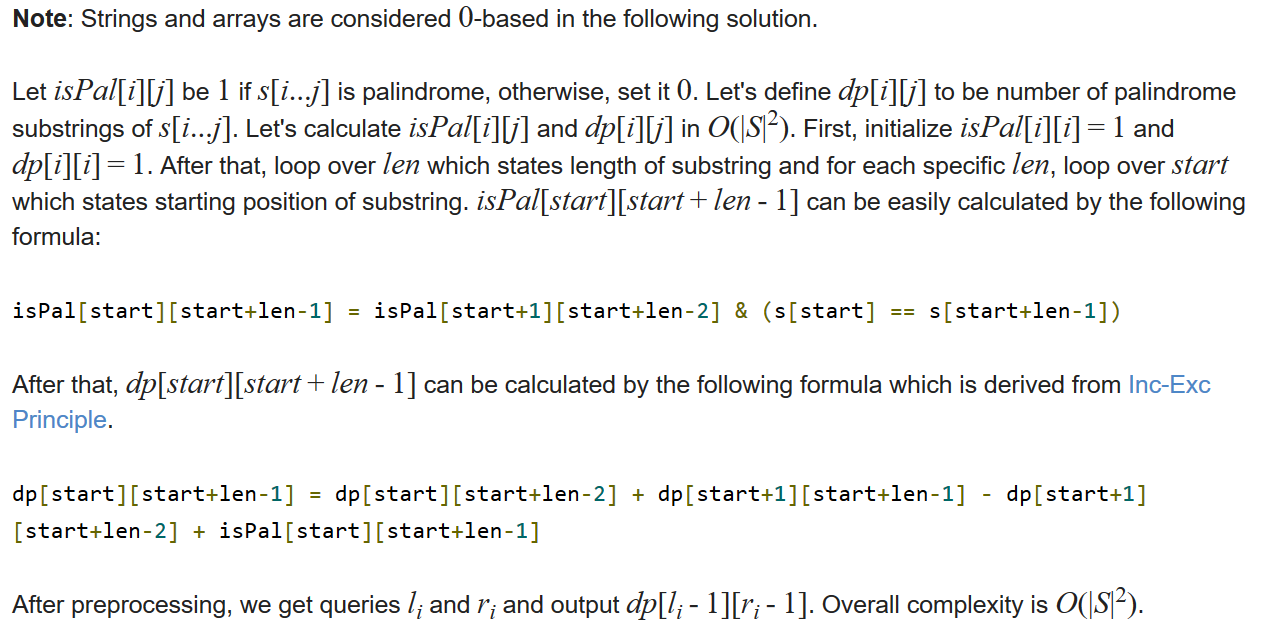
\includegraphics[width=0.5\textwidth,height=0.5\textheight,keepaspectratio]{palsub} 	
	\item \href {https://github.com/sourabh2311/Competitive-Programming/blob/master/HimanshuSA11107.cpp}{UVA 11107 Sol - simple}, \href {https://github.com/sourabh2311/Competitive-Programming/blob/master/HimanshuSA11107.cpp}{UVA 11107 Sol - complicated but more powerful}: Problem is to find the longest substring shared by more than half of given strings.	
	\item \href {https://gist.github.com/sourabh2311/25edb7a7067948832ade9192bd2635ce}{UVA 10459 Sol}, \href {https://uva.onlinejudge.org/external/104/10459.pdf}{UVA 10029 Prob}: Edit steps, (lexicographic sequence of words)	
\end{itemize}
\section{Geometry}
\begin{itemize}
    \item for given 3 points of a valid parallelogram, there are 3 possible locations for the 4th point.
    \item we have a hexagon with integral sides and all interior angles equal to 120 deg. we draw lines parallel to the side of the hexagon, such that we get equilateral triangles of side 1 unit, how many equilateral triangles did we got? Sol: 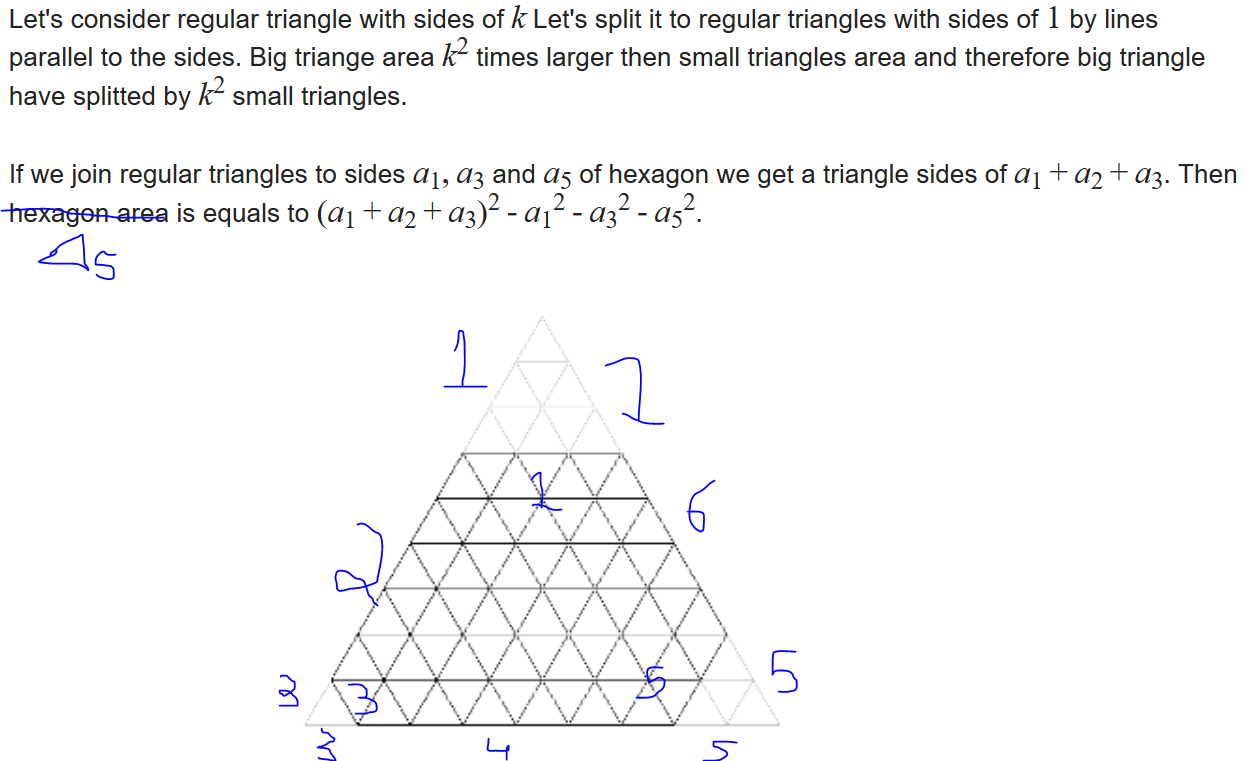
\includegraphics[width=0.5\textwidth,height=0.5\textheight,keepaspectratio]{triangle} 
    \item An inscribed angle is an angle formed by 2 chords in a circle which have a common endpoint. This common endpoint form the vertex o the inscribed angle. The other 2 endpoints define what we call an intercepted arc.
    \item Measure of intercepted arc of a unit circle is $2/\pi$ that of inscribed angle.
    \item 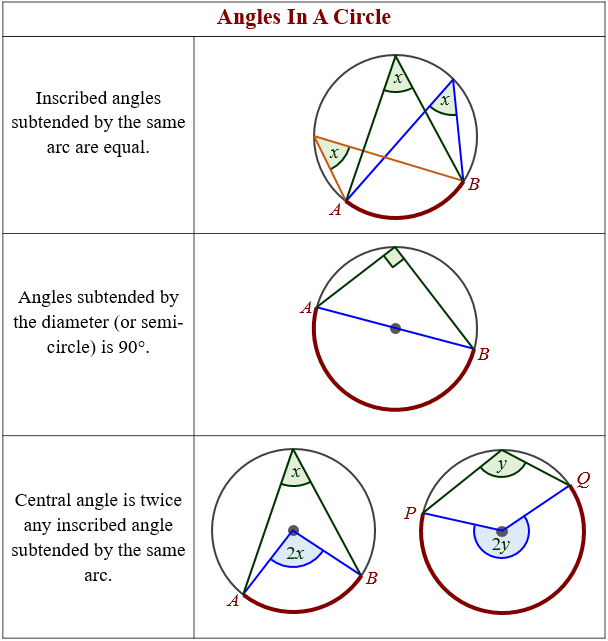
\includegraphics[width=0.5\textwidth,height=0.5\textheight,keepaspectratio]{basiccircle} 
    \item Circles will certainly not touch or intersect iff the dist. between their center is greater than the sum of their radii.
    \item A circle 'a' contains a circle 'b' iff the distance between their centers is less than the absolute value of their radii difference.
    \item let the bottom left/top right corner point be denoted as a/c resp. Then rectangles intersect iff $max(a1.x, a2.x) < min(c1.x, c2.x)$ and $max(a1.y, a2.y) < min(c1.y, c2.y)$.
    \item Similarly in case of 3d, vol of intersection of all cuboids is given by $(ux - lx)(uy - ly)(uz - lz)$ where lx = max(x1, x2, ..., xn) and ux = min(...).
    \item To get unique points 
    \begin{minted}{cpp}
    sort(cops.begin(), cops.end());
    cops.resize (distance(cops.begin (), unique (cops.begin(), cops.end())))
    \end{minted}
    \item Remember that we can apply bisection method ($while (abs(hi - lo) < eps$) and ternary search in geometry.
    \item for a quadrilateral drawn inside circle sum of opposite angles is 180 deg.
    \item Sum of all angles of a quadrilateral is always 360 deg.
    \item Center of mass of pts $= \sum m_i \vec{r_i}/\sum{m_i}$. This is same as centre of mass of union of mutually exclusive objects where each $\vec{r_i}$ is that objects COM and $m_i$ is that objects mass.
    \item COM of a line is its midpoint
    \item COM of $\triangle = (\vec{r_1} + \vec{r_2} + \vec{r_3}) / 3$ but this is not the case for general polygon.
    \item For a general convex polygon, we may triangulate it, find that triangles area and COM and the combine to get COM of original figure.
    \item Similarly in case of 3D, COM of tetrahadron $= \sum_{i = 1}^{4}r_i/4$ and a general 3d object can be again divided into tetrahedrons.
    \item For general polygon we can do $\vec{r_c} = (\sum_{i}\vec{r_{z,p_i, p_{i + 1}}} * S_{z, p_i, p_{i + 1}}) / \sum_i S_{z, p_i, p_{i + 1}}$ where S term denotes triangles area with sign. 
    \item \textbf{Some properties of triangles}
    \begin{itemize}
        \item $s = p/2$
        \item $A = \sqrt{s*(s - a)*(s - b)*(s - c)}$
        \item $a/\sin{A} = b/\sin{B} = c/\sin{C} = 2*R$
        \item $R = abc/(4*A)$
        \item $c^2 = a^2 + b^2 - 2*a*b*\cos(C)$
        \item Inscribed circle (incircle), $r = A/s$
        \item Center of incircle is the meeting point of angle bisectors.
        \item Medians divide a triangle into 6 triangles of equal area and area of original triangle is $= 4/3 * \sqrt{s * (s - a) * (s - b) * (s - c)}$, here a, b, c is the length of medians.
        \item For valid $\triangle$ sum of any 2 sides should be greater than third. If the three lengths are sorted, we can simply check whether $a + b > c$. For quadrangle sum of any 3 sides should be greater than 4th.
        \item The center of circumcircle is the meeting point of $]triangle$'s perpendicular bisector.
        \item Triangle angle bisector property: $|AB|/|AC| = |BD|/|DC|$ where AD is the angle bisector of angle BAC. 
        \item Given sides of triangle, sort them, then see 3 consecutive sides, if the area is positive (using herons formula), they form a valid triangle, mx = max (mx, area).
    \end{itemize}
    \item Kite is a quadrilateral which has two pair of sides of same length which are adjacent to each other. The area of kits is $diagonal_1*diagonal_2/2$. Diagonals of kite are perpendicular.
    \item Rhombus is a special parallelogram where every side has equal length. It is also a special case of kits where every side has equal length.    
    \item Convex Polygon: All interior angles should be less than 180 deg. Polygon which is not Convex is Concave
    \item Concave polygon has critical point (point from which entire polygon is not visible).
    \item \textbf{Pick's Theorem}. $A=i+\frac{b}{2}-1$, where: $P$ is a simple polygon whose vertices are grid points, $A$ is area of $P$, $i$ is \# of grid points in the interior of $P$, and $b$ is \# of grid points on the boundary of $P$. \\
    If $h$ is \# of holes of $P$ ($h+1$ simple closed curves in total), $A=i+\frac{b}{2}+h-1$.
    \begin{minted}{cpp}
// way to get boundary points

ll getb (vector<point> &poly) {
    ll b = 0;
    int n = P.size () - 1;
    for (int i = 0; i < n ;i++) {
        int j = i + 1; 
        ll ret = gcd (abs(poly[i].x - poly[j].x), abs (poly[i].y - poly[j].y));
        // for point to be on lattice its x and y coordinate has to be a multiple of gcd.
        b += ret;
    }
    return b;
}
    \end{minted}
    \item To check whether a point is on or inside a polygon that area method is best.
    \item Centroid of a polygon, $C_x = 1/(6*A)*\sum_{i = 0}^{n - 1}(x_i + x_{i + 1}) * (x_i * y_{i + 1} - x_{i + 1} * y_i)$
    \\$C_y = 1/(6*A)*\sum_{i = 0}^{n - 1}(y_i + y_{i + 1}) * (x_i * y_{i + 1} - x_{i + 1} * y_i)$
    \\\textbf{Here: }$(x_n, y_n) = (x_0, y_0)$. And dont given absolute value to A.
    \item \[A = 1/2\begin{bmatrix}
    x_0 & y_0\\
    x_1 & y_1\\
    \vdots & \vdots\\
    x_n & y_n
    \end{bmatrix} = 1/2 * ((x_0 * y_1 + x_1 * y_2 + \dots + x_{n - 2} * y_{n - 1}) - (x_1*y_0 \dots)\]
    \item 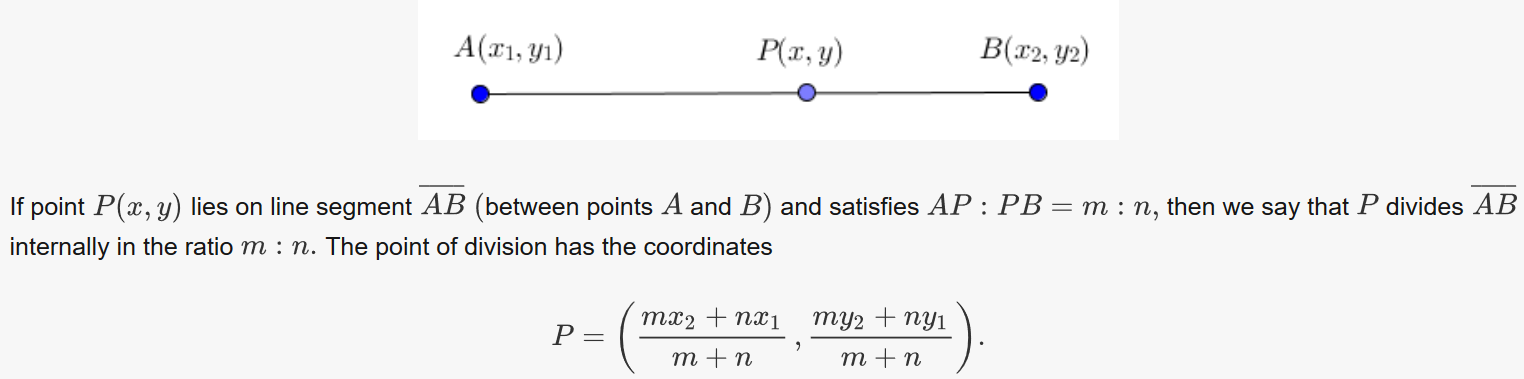
\includegraphics[width=0.5\textwidth,height=0.5\textheight,keepaspectratio]{p1} 
    \item 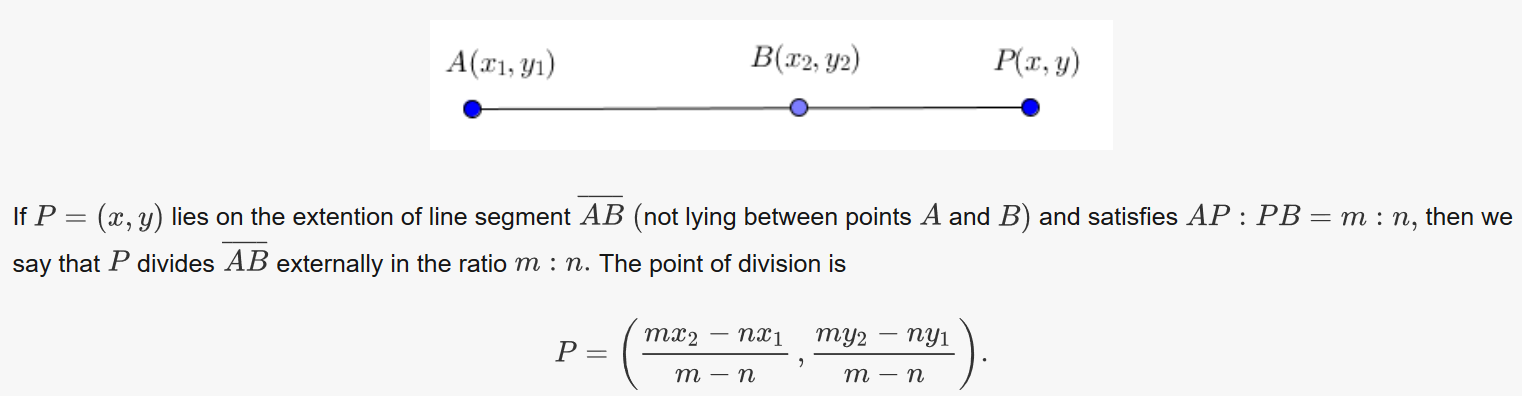
\includegraphics[width=0.5\textwidth,height=0.5\textheight,keepaspectratio]{p2}
    \item \href{https://github.com/sourabh2311/Competitive-Programming/blob/master/Libs/areaOfUnionOfTriangles.cpp}{Area of union of triangles}
    \item \href{http://e-maxx.ru/algo/circle_tangents}{Finding common tangents to two circles}
    \item \href{https://uva.onlinejudge.org/external/101/10173.pdf}{Minimum Bounding Rectangle}, \href{https://github.com/sourabh2311/Competitive-Programming/blob/master/UVA_10173.cpp}{Sol}: basically use atan2 and rotate wrt that point.
    \item Given a set of points, to determine whether a point lies inside a triangle formed by any 3 points, it is enough to check whether the given point lies inside the convex hull of given data points.
\end{itemize}
\subsection{Fast application of a set of geometric operations to a set of points}
\begin{itemize}
    \item Given n points $p_i = [x_i, y_i, z_i]$, apply m transformations to each of these points. Each transformation can be a shift, a scaling or a rotation around a given axis by a given angle. There is also a "loop" operation which applies a given list of transformations k times. ("loop" operations can be nested) All the operations should be applied faster than $O(n * length)$, where length is the total no. of transformations to be applied (after unrolling "loop" operations).
    \\ Sol. Each of the transformation can be written as a linear combination of old coordinates giving us a 4x4 matrix.
    \item point is represented as $[x, y, z, 1]$ and here I am multiplying operation to the right of the point (actually I should have done it as a transpose of whole thing)
    \item Shift x by 5, y by 7, z by 9.
    \[\begin{bmatrix}
    1 & 1 & 0 & 0\\
    0 & 1 & 0 & 0\\
    0 & 0 & 1 & 0\\
    5 & 7 & 9 & 1
    \end{bmatrix}\]
    \item Scale x by 10 other two by 5.
    \[\begin{bmatrix}
    10 & 0 & 0 & 0\\
    0 & 5 & 0 & 0\\
    0 & 0 & 5 & 0\\
    0 & 0 & 0 & 1
    \end{bmatrix}\]
    \item Rotate $\theta$ deg. around x axis.
    \[\begin{bmatrix}
    1 & 1 & 0 & 0\\
    0 & \cos{\theta} & -\sin{\theta} & 0\\
    0 & \sin{\theta} & \cos{\theta} & 0\\
    0 & 0 & 0 & 1
    \end{bmatrix}\]
    \item Now, once every transformation is described as a matrix, the sequence of transformations can be described as a product of these matrices and a "loop" of k repetitions can be described as the matrix raised to the power k (which can be calc. using binary exponentiation). Time complexity $O(n + m * \log{k})$.
\end{itemize}
\subsection{Klee's Algo}
Given $n$ segments on a line, each described by a pair of coordinates $(a_{i1}, a_{i2})$. We have to find the length of their union.
\\It works in $O(n\log n)$ and has been proven to be the asymptotically optimal.
\begin{minted}{cpp}
// Returns sum of lengths covered by union of given 
// segments 
int segmentUnionLength(const vector <pair <int,int> > &seg) {
    int n = seg.size(); 
    // Create a vector to store starting and ending 
    // points 
    vector <pair <int, bool> > points(n * 2); 
    for (int i = 0; i < n; i++) 
    { 
        points[i*2]     = make_pair(seg[i].first, false); 
        points[i*2 + 1] = make_pair(seg[i].second, true); 
    } 
  
    // Sorting all points by point value 
    sort(points.begin(), points.end()); 
  
    int result = 0; // Initialize result 
  
    // To keep track of counts of current open segments 
    // (Starting point is processed, but ending point 
    // is not) 
    int Counter = 0; 
  
    // Trvaerse through all points 
    for (int i=0; i<n*2; i++) 
    { 
        // If there are open points, then we add the 
        // difference between previous and current point. 
        // This is interesting as we don't check whether 
        // current point is opening or closing, 
        if (Counter) 
            result += (points[i].first - points[i-1].first); 
  
        // If this is an ending point, reduce, count of 
        // open points. 
        (points[i].second)? Counter-- : Counter++; 
    } 
    return result; 
} 
\end{minted}
\subsection{Closest Pair Problem}
\revised
\begin{minted}{cpp}
// First sort the points by their x coordinates. Do whatever if there is tie.
// I have to write the correct implementation following the idea mentioned in cormen and use it to solve codejams prob.
// Commented section shows how to solve the problem: 
// Find out the maximum size such that if you draw such size quared around each point (that point will be at the center of the square) and no two squared will intersct each other (cna touch but not intersect). To make the problem simple the sides of the square will be parallel to X and Y axis.
double dvac(int low, int high) {
   if(low < high) {
       if(low == high - 1) {
           return dist(data[low], data[high]);  // return max (data[high].x - data[low].x, abs (data[high].y - data[low].y));  
       }
       int mid = (low + high) / 2;
       double d1 = dvac(low, mid);
       double d2 = dvac(mid + 1, high);
       double dp = min(d1, d2);
       double d3 = 10000;
       // It is guarenteed that there can be atmost 6 points
       for(int i = mid; i >= low; i--) {
           double temp = dist(point(data[i].x, 0), point(data[mid].x, 0));
           if(temp > dp - EPS) break;
           for(int j = mid + 1; j <= high; j++) {
               double temp2 = dist(point(data[i].x, 0), point(data[j].x, 0));
               if(temp2 > dp - EPS) break;
               d3 = min(d3, dist(data[i], data[j]));
               // d3 = min (d3, max (data[j].x - data[i].x, abs(...));)
           }
       }
       return min(dp, d3);
   }
   return 10000;
}

\end{minted}
\end{document}
